\documentclass[TS]{sesamanuel}

% modifications dans la classe (fichier sesamanuel.cls) :
% 	1) ligne 2873, la ligne de remise à zéro du compteur de chapitre a été commentée pour "themaG"
% 	2) création d'une boîte à connaître à la ligne 3471
%	3) ligne 2141 : définition de trois couleurs utilisé par les anciennes figures libreoffice
%	4) ligne 179 et 180 ajout de 2 lignes pour utiliser la police pazocal qui modifie les caractères calligraphiés en mode math
%		du coup : \mathcal{C} donne un C fortement calligraphié et \pazocal{C} donne l'habituel C calligraphié de mathcal
%	5) suppression du texte et du logo dans le titre des QCM d'autoévaluation "Ressources dispo sur sesamaths..." :
%		lignes 3117 et 4396 : commande \StringManuel est commentée
%		lignes 3122 et 4401 : je n'ai pas supprimé le \LogoManuel (une @) mais j'ai changé sa couleur de U4 à Blanc (à la ligne 2702)

% modifications dans le fichier commandesTikZ :
% lignes 31 et 32 pour ajouter la commande \circled qui entoure un caractère



%%%%%%%
%Rajouté le 12/06/2018 SV et BN pour compilation espace insécable sous linux 
\DeclareUnicodeCharacter{00A0}{~} %pour remplacer les espaces insécables
\DeclareUnicodeCharacter{2011}{-}
%\usepackage{pdfpages}
%%%%%%%


%#######################################################################
%################# Options de compilation
%#######################################################################

\def\ChoixDeVersion{eleve} % soit {prof} et alors les commentaires profs sont ajoutés, soit autre chose

\newcommand{\prof}[1]{
        \ifthenelse{
                \equal{\ChoixDeVersion}{prof}
                }{\vspace{6pt}
                
                \vspace{12pt}
\includegraphics[angle=0,width=1.5cm]{./Images/prof} \textbf{Professeur :} \textsl{#1}
                
                \vspace{12pt}}{}
}

% remarque : pour compiler
% latex --jobname=NomFichierSortie '\def\ChoixDeVersion{prof}\input{FichierSource.tex}'      



\input{commandes-manuel-TS} % pour l'instant on garde sinon les corrigés ne sont
						% pas dans classés dans un dossier "correction"

\usepackage{esvect,cancel} 
\newcommand{\chapeaumelon}[1]{\stackrel{\Large \frown}{#1}}

%%%%%%%% pour les figures en tikz
\usepackage{tikz,xparse}%xparse ajouté pour le compas
\usepackage{tkz-tab,tkz-euclide}
\usetkzobj{all}
\usepackage{pgf}
\usetikzlibrary{calc} %pour mettre des calculs dans les coordonnées de points
\usetikzlibrary{arrows}
\usetikzlibrary{patterns}  
\usetikzlibrary{intersections}%pour l'utilisation de l'intersection de 2 figures
\usetikzlibrary{shapes.geometric}
\usepackage{tikzpeople}
%\usepackage{tikzducks}

\definecolor{CyanTikz40}{cmyk}{.4,0,0,0}
\definecolor{CyanTikz20}{cmyk}{.2,0,0,0}

\definecolor{B1prime}      {cmyk}{0.00, 1.00, 0.00, 0.50}
\definecolor{H1prime}      {cmyk}{0.50, 0.00, 1.00, 0.00}

\tikzstyle{general}         =[font=\fontsize{7.5}{9}\selectfont,line width=0.3mm, >=stealth, x=1cm, y=1cm,line cap=round, line join=round]
\tikzstyle{quadrillage}     =[line width=0.3mm, color=CyanTikz40]
\tikzstyle{quadrillageNIV2} =[line width=0.3mm, color=CyanTikz20]
\tikzstyle{quadrillage55}   =[line width=0.3mm, color=CyanTikz40, xstep=0.5, ystep=0.5]
\tikzstyle{cote}            =[line width=0.3mm, <->]
\tikzstyle{epais}           =[line width=0.5mm, line cap=butt]
\tikzstyle{tres epais}      =[line width=0.8mm, line cap=butt]
\tikzstyle{axe}             =[line width=0.3mm, ->, color=Noir, line cap=rect]
\newcommand{\quadrillageSeyes}[2]{%
  \draw[line width=0.3mm, color=A1!10, ystep=0.2, xstep=0.8] #1 grid #2;
  \draw[line width=0.3mm, color=A1!30, xstep=0.8, ystep=0.8] #1 grid #2;
}

% ajouter pour manuel Flo
\newcommand*\circled[1]{\tikz[baseline=(char.base)]{
	\node[shape=circle,draw,inner sep=1pt] (char) {#1};}}

\newcommand{\axeX}[4][0]{%
  \draw[axe] (#2,#1)--(#3,#1);
  \foreach \x in {#4} {\draw (\x,#1) node {\small $+$};
    \draw (\x,#1) node[below] {\small $\numprint{\x}$};
  }%
}
\newcommand{\axeY}[4][0]{%
  \draw[axe] (#1,#2)--(#1,#3);
  \foreach \y in {#4} {\draw (#1, \y) node {\small $+$};
    \draw (#1, \y) node[left] {\small $\numprint{\y}$};
  }%
}
\newcommand{\axeOI}[3][0]{%
  \draw[axe] (#2,#1)--(#3,#1);
  \draw (1,#1) node {\small $+$};
  \draw (1,#1) node[below] {\small $I$};
}
\newcommand{\axeOJ}[3][0]{%
  \draw[axe] (#1,#2)--(#1,#3);
  \draw (#1, 1) node {\small $+$};
  \draw (#1, 1) node[left] {\small $J$};
}
\newcommand{\axeXgraduation}[2][0]{%
  \foreach \x in {#2} {\draw (\x,#1) node {\small $+$};}%
}
\newcommand{\axeYgraduation}[2][0]{%
  \foreach \y in {#2} {\draw (#1, \y) node {\small $+$};}%
}
\newcommand{\origine}{%
  \draw (0,0) node[below left] {\small $0$};
}
\newcommand{\origineO}{%
  \draw (0,0) node[below left] {$O$};
}
\newcommand{\point}[4]{%
  \draw (#1,#2) node[#4] {$#3$};
}
\newcommand{\pointGraphique}[4]{%
  \draw (#1,#2) node[#4] {$#3$};
  \draw (#1,#2) node {$+$};
}
\newcommand{\pointFigure}[4]{
  \draw (#1,#2) node[#4] {$#3$};
  \draw (#1,#2) node {$\times$};
}
\newcommand{\pointC}[3]{
  \draw (#1) node[#3] {$#2$};
}
\newcommand{\pointCGraphique}[3]{
  \draw (#1) node[#3] {$#2$};
  \draw (#1) node {$+$};
}
\newcommand{\pointCFigure}[3]{
  \draw (#1) node[#3] {$#2$};
  \draw (#1) node {$\times$};
}

\newcommand{\NodeAngle}[2]{%
    %\pgfextra{
        \pgfmathanglebetweenpoints%
            {\pgfpointanchor{#1}{center}}%
            {\pgfpointanchor{#2}{center}}%
            \global\let\MyAngle\pgfmathresult
    }%}

    % #1 premier point              ---- Distance entre 2 nodes ----
    % #2 second point
    % On récupère le résultat dans \MyDist
\makeatletter
\newcommand{\NodeDist}[2]{%
    \pgfpointdiff{\pgfpointanchor{#1}{center}}
                 {\pgfpointanchor{#2}{center}}
    % no need to use a new dimen
    \pgf@xa=\pgf@x
    \pgf@ya=\pgf@y
    % to convert from pt to cm   
    \pgfmathparse{veclen(\pgf@xa,\pgf@ya)/28.45274}
    \global\let\MyDist\pgfmathresult % we need a global macro   
}
\makeatother

% ######################
%     Dessin crayon    #
% ######################

\newcommand{\Crayon}[1]{%
    \begin{scope}[scale=.7,#1]
    \fill[gray!60] (-.2,4.8) -- (.2,4.8)
                -- (.2,.8) --(.1,.65)
                -- (0,.8) -- (-.1,.66)
                -- (-.2,.8) -- cycle ;
    \draw[color=white] (0,4.8) -- (0,.8 );
    \fill[black] (-.2,4.3) -- (0,4.27)
                -- (.2,4.3) -- (.2,4.8) arc(30:150:0.23cm) ;
    \fill[brown!50] (-.2,.8)
        -- (0,0) node[coordinate,pos=0.75](a){}
        -- (.2,.8) node[coordinate,pos=0.25](b){}
        -- (.1,.65) -- (0,.8) -- (-.1,.66) -- cycle;
    \fill[gray] (a) -- (0,0) -- (b) -- cycle;
    \end{scope}
}



% ######################
%   Dessin du compas   #
% ######################

\NewDocumentCommand{\Compas}{smm}{%

    \IfBooleanTF{#1}{%
    % with *
    % keep distance between extemities
    }{%
    % without *
    % calulation of the distance between extemities
    \NodeDist{#2}{#3}
    }

    \NodeAngle{#2}{#3}

    \def\L{6} % taille des branches du compas

    % calcul de l'angle de l'ouverture
    \pgfmathsetmacro{\AngleCP}{asin(\MyDist/(2*\L))}

    \begin{scope}[shift=(#2)]
    \begin{scope}[%
        join=round,
        rotate=\MyAngle,
        shift=(270-\AngleCP:-\L)
        ]

    % branche pointe sèche
    \draw[rotate=-\AngleCP,fill=gray!80]
        (0,0)--(0,-\L)--(-.2,-\L+.8)--(-.2,0)--cycle ;
    \draw[rotate=-\AngleCP,fill=gray!05]
        (0,-\L+.8)--(0,-\L)--(-.2,-\L+.8)--cycle ;

    % branche crayon
    \draw[rotate=\AngleCP,fill=gray!80]
        (0,0)--(0,-\L)--(.2,-\L+.8)--(.2,0)--cycle ;

    \begin{scope}[rotate=\AngleCP,shift={(0,-\L)}]
    \Crayon{rotate=-12}
    \draw[fill=gray!25] (\L/30,\L/5) circle (\L/36) ;
    \fill[gray!5] (\L/30,\L/5)
            -- ++(30:\L/36) arc (30:45:\L/36) -- cycle ;
    \fill[gray!5] (\L/30,\L/5)
            -- ++(210:\L/36) arc (210:225:\L/36) ;
    \filldraw (\L/30,\L/5) circle (.02) ;
    \end{scope}

    % haut du compas
    \draw[fill=gray!80] (-.1,0) rectangle (.1,.7) ;
    \draw[fill=gray!25] (0,0) circle (.25) ;
    \fill[gray!5] (0,0) -- (30:.25) arc (30:45:.25) -- cycle ;
    \fill[gray!5,rotate=180] (0,0) -- (30:.25) arc (30:45:.25) -- cycle ;
    \filldraw (0,0) circle (.05) ;
    \end{scope}
    \end{scope}
}




\graphicspath{%
  {ex1/figures/}%
  {NombresEntiersDecimaux/figures/}%
  {OperationsNombresEntiersDecimaux/figures/}%
  {PointsSegmentsDroites/figures/}%
  {PrioritesOperations/figures/}%
  {Triangles/figures/}%
  {NbsEntiers_Multiples_Diviseurs/figures/}%
  {Quadrilateres/figures/}%
  {NbsRelatifs/figures/}%
  {PerimetresAires/figures/}%
  {Images/}%
}


% création d'un nouveau thème "calcul" pour le document
\NewThema{C}{c}{calcul}{Calcul}{CALCUL}{PartieFonction}{A3}

\renewcommand\ListeMethodesThemes{{c}{C},{g}{G}}
\renewcommand*\StringListeMethode{M\'ethodes du livret 1}

% création d'un nouveau thème "Manuel" pour le sommaire
\NewThema{M}{m}{manuel}{Manuel}{MANUEL}{PartieFonction}{A3}

\DecimalMathComma
\begin{document}

%%%%%%%%%%%%%%%%%%%%%%
%Couverture inclusion page entière en eps
\pagestyle{empty}

\includegraphics[width=.92\textwidth]{couverture}

\newpage \pagestyle{empty}
\addto\captionsfrench{\renewcommand{\contentsname}{Sommaire}}

%\setcounter{tocdepth}{2}


%%%%%%%%%%%%%%%%%%%%%%%%%%
% Table des matières
%%%%%%%%%%%%%%%%%%%%%%%%%%
\themaM %thème déclaré en début de document
\colorlet{ChapterNumColor}{PartieFonction}
\chapter{Manuel de 6e\\Tome 1}

\vfill
\begin{commentaire}


\textcolor{PartieFonction}{\PrerequisTitleFont 
Chapitre \ref{ChNbEntiersDecimaux}: Rappels sur les Nombres \dotfill\ page\pageref{ChNbEntiersDecimaux}}

\vspace{2em}

\textcolor{PartieFonction}{\PrerequisTitleFont 
Chapitre \ref{ChOpNbEntDec}: Opérations avec les nombres décimaux \dotfill\ page \pageref{ChOpNbEntDec}}

\vspace{2em}

\textcolor{PartieGeometrie}{\PrerequisTitleFont 
Chapitre \ref{ChDroitesAngles}: Points, segments, droites et angles \dotfill\ page \pageref{ChDroitesAngles}}

\vspace{2em}

\textcolor{PartieFonction}{\PrerequisTitleFont 
Chapitre \ref{ChPrioritesOperations}: Priorités des opérations \dotfill\ page \pageref{ChPrioritesOperations}}

\vspace{2em}

\textcolor{PartieGeometrie}{\PrerequisTitleFont 
Chapitre \ref{ChTriangles}: Triangles \dotfill\ page \pageref{ChTriangles}}

\vspace{2em}

\textcolor{PartieFonction}{\PrerequisTitleFont 
Chapitre \ref{ChNbEntiersMultDiv}: Nombres entiers, multiples, diviseurs \dotfill\ page \pageref{ChNbEntiersMultDiv}}

\vspace{2em}

\textcolor{PartieGeometrie}{\PrerequisTitleFont 
Chapitre \ref{ChQuadrilateres}: Quadrilatères \dotfill\ page \pageref{ChQuadrilateres}}

\vspace{2em}

\textcolor{PartieFonction}{\PrerequisTitleFont 
Chapitre \ref{ChNbRelatifs}: Nombres relatifs \dotfill\ page \pageref{ChNbRelatifs}}

\vspace{2em}

\textcolor{PartieGeometrie}{\PrerequisTitleFont 
Chapitre \ref{ChPerimetresAires}: Périmètres et aires \dotfill\ page \pageref{ChPerimetresAires}}

\vspace{2em}
\textcolor{PartieFonction}{\PrerequisTitleFont 
Chapitre \ref{ChDurees}: Opérations sur les durées \dotfill\ page\pageref{ChDurees}}

\end{commentaire}
\vfill
%%%%%%%%%%%%%%%%%%%%%%%%%%
% Fin table des matières
%%%%%%%%%%%%%%%%%%%%%%%%%%

%%%%%%%%%%%%%%%%%%%%%%%%%%
%Page Sesamath
%%%%%%%%%%%%%%%%%%%%%%%%%%
\newpage


\begin{prerequis}[Un manuel de l'association Sésamath]
\begin{itemize}
\item  Ce manuel est adapté en partie du manuel Sésamath de l'association Sésamath:\\
\texttt{http://manuel.sesamath.net/}
\item … Et de l'association Sésamath Suisse romande:\\ \texttt{http://www.sesamath.ch/}
\item L'Institut Florimont a réalisé la transcription dans le langage de description de documents libre et gratuit \LaTeX{} en utilisant la classe \texttt{sesamanuel} développée par l'association Sésamath;
\item E. Villié a réalisé la couverture pour l'Institut Florimont;
\item Version Septembre 2019 --- Institut Florimont (Genève);\vspace{0.3em}
\item Publication sous licence libre \hspace{1em} \raisebox{-0.4\height}{\includegraphics[width=2cm]{cc-by-sa}}
\end{itemize}
 \end{prerequis}

\vspace{1em}




%%%%%%%%%%%%%%%%%%%%%%%%%%
%Fin page Sesamath
%%%%%%%%%%%%%%%%%%%%%%%%%%

\colorlet{ChapterNumColor}{white}
\setcounter{chapter}{0}

\setcounter{page}{4}

\themaG
%\prof{
\chapter{Bonnes Idées}\label{ChBonnesIdees}

Cette page contient les bonnes idées collectées avec les années. N'hésitez pas à l'enrichir de VOS bonnes idées...\\

\begin{itemize}
    \item Penser à faire faire aux élèves des affiches qui pourront être accrochées dans la classe.
    \item On peut proposer aux élèves de faire des présentations, des exposés sur différents thèmes. Dans ce cas, penser à leur donner une trame ou les exigences que vous avez.
\end{itemize}

%}

\themaC

\chapter{Les ensembles de nombres}\label{ChEnsemblesnombres}

\begin{center}
   \includegraphics{Ensemblesnombres/figures/ensembles.tex} 
\end{center}


%\themaC
%\chapter{Rappels sur les nombres}\label{ChNbEntiersDecimaux}

\begin{acquis}
\begin{itemize}
\item lire et écrire des nombres décimaux en chiffres;
\item déterminer le chiffre des dizaines, des unités, des dixièmes, des centièmes… d'un nombre décimal;
\item déterminer le nombre de dizaines, d’unités, de dixièmes, de centièmes… d'un nombre décimal;
\item connaître la définition d'une fraction et le vocabulaire s'y rapportant;
\item savoir passer de l'écriture décimale à une écriture fractionnaire d'une quantité et inversement;
\item placer des nombres décimaux sur une droite graduée et lire les abscisses de nombres décimaux placés sur une droite graduée (sous forme décimale ou fractionnaire);
\item classer des nombres décimaux par ordre croissant et décroissant en utilisant les symboles < ou >;
\item encadrer un nombre décimal à une précision donnée;
\item déterminer l'arrondi d'un nombre décimal à une précision donnée;
\end{itemize}
\end{acquis}

\cours
\section{Le système décimal}

% remarque : pour qu'un mot se retrouve dans le lexique : \MotDefinition{asymptote horizontale}{}
Les règles et conventions qui permettent d'écrire et de lire les nombres forment ce qu'on appelle un \textbf{système de numération}. Nous utilisons le système décimal, de base dix.

\begin{aconnaitre}
Pour écrire les chiffres dans le système décimal, il nous faut dix symboles, appelés des \emph{chiffres}. Ces chiffres sont :
\[ 0\,;\,1\,;\,2\,;\,3\,;\,4\,;\,5\,;\,6\,;\,7\,;\,8\,;\,9  \]
Il arrive parfois qu'on confonde \textbf{\MotDefinition{chiffre}{}} et \textbf{\MotDefinition{nombre}{}}. On peut faire l'analogie avec l'écriture d'une langue en affirmant que les \textbf{\textcolor{H1}{chiffres}} sont des \textbf{\textcolor{H1}{lettres}} et que les \textbf{\textcolor{H1}{nombres}} sont des \textbf{\textcolor{H1}{mots}}. Ainsi, 13 est un nombre qui s'écrit avec les chiffres 1 et 3.
\end{aconnaitre}

%%%%%%%%%%%%%%%%%%%%%%%%%%%%%%%%%%%%%%%%%%%%%%%%%%%%%%%%%%%%%%%%%%%%%%%%%%%
\prof
{Il est très important que les élèves fassent la différence entre chiffre et nombre pour la suite du chapitre. Ils ont sans doute appris autre chose à l'école primaire donc il faut découstruire ce faux-savoir.}
%%%%%%%%%%%%%%%%%%%%%%%%%%%%%%%%%%%%%%%%%%%%%%%%%%%%%%%%%%%%%%%%%%%%%%%%%%%

Un \textbf{\textcolor{C2}{nombre décimal}} est un nombre qui s'écrit en deux parties séparées par une virgule (écriture décimale).

\hspace{2em}\textbullet\hspace{.25em} la partie entière, à gauche de la virgule. Elle correspond au nombre d'unités entières contenues dans le nombre.

\hspace{2em}\textbullet\hspace{.25em} la partie décimale, à droite de la virgule. Elle correspond à une portion d'unité supplémentaire.

De ce fait:

\begin{center}
\textbf{\textcolor{C2}{nombre décimal = partie entière + partie décimale}}
\end{center}

Un nombre entier est caractérisé par le fait qu'il n'a pas de partie décimale (on omet alors la virgule).


\begin{methode*1}[Tableau des nombres]
\begin{exemple*1}

Soit le nombre 34 567,19

\hspace{2em}\textbullet\hspace{.25em} Partie entière: 34 567
 
\hspace{2em}\textbullet\hspace{.25em} Partie décimale: 0,19


\end{exemple*1}

\exercice

Soit le nombre 10,153.

\hspace{2em}\textbullet\hspace{.25em}Partie entière: \dotfill

\hspace{2em}\textbullet\hspace{.25em} Partie décimale:\dotfill

\exercice

Compléter le tableau suivant pour les nombres 10,01 ; 0,037 ; 200 000 042 000.

\vspace{2em}

\begin{ttableau}{\linewidth}{19}
\hline
\multicolumn{3}{|c|}{milliards} & \multicolumn{3}{c|}{millions} & \multicolumn{3}{c|}{mille} & 
\multicolumn{3}{c|}{unités} & 
\multirow{2}{*}{\parbox{\linewidth}{ \vspace{1.5cm} \textcolor{B1}{  \textbf{,} }  }} &  %ADD PARBOX !!
\multirow{2}{*}{\rotatebox{90}{\phantom{dixièmes}}} &
\multirow{2}{*}{\rotatebox{90}{\phantom{centièmes}}} & 
\multirow{2}{*}{\rotatebox{90}{\phantom{millièmes}}} & 
\multirow{2}{*}{\rotatebox{90}{\phantom{dix-millièmes}}} & 
\multirow{2}{*}{\rotatebox{90}{\phantom{cent-millièmes}}} &
\multirow{2}{*}{\rotatebox{90}{\phantom{millionièmes}}} \\ \cline{1-12}
\rotatebox{90}{\phantom {centaines de ...}} & 
\rotatebox{90}{\phantom {dizaines de ...}} & 
\rotatebox{90}{\phantom {unités de ...}} &
\rotatebox{90}{\phantom {centaines de ...}} & 
\rotatebox{90}{\phantom {dizaines de ...}} & 
\rotatebox{90}{\phantom {unités de ...}} &
\rotatebox{90}{\phantom {centaines de ...}} & 
\rotatebox{90}{\phantom {dizaines de ...}} & 
\rotatebox{90}{\phantom {centaines de ...}} &
\rotatebox{90}{\phantom {dizaines de ...}} & 
\rotatebox{90}{\phantom {unités de ...}} & 
 & & & & & &       &   \\ \hline  % ADD EXTRA & ON THIS LINE B4 \\ \hline !!
& & & & & 3 & 0 & 2 & 7 & 4 & 6 & 2 & \textcolor{B1}{\textbf{,}} & 0 & 0 & 0 & 0 & 0 & 0 \\ \hline
& & & & & & & & & & & & \textcolor{B1}{\textbf{,}} & & & & & &\\ \hline
& & & & & & & & & & & & \textcolor{B1}{\textbf{,}} & & & & & &\\ \hline
& & & & & & & & & & & & \textcolor{B1}{\textbf{,}} & & & & & &\\ \hline
\end{ttableau}
\end{methode*1}

\begin{remarque}

\hspace{2em}\textbullet\hspace{.25em} La partie décimale est toujours finie: on peut compter les chiffres après la virgule.

\hspace{2em}\textbullet\hspace{.25em} Lorsque la partie décimale n'est pas finie, on a un nombre infini qui n'est PAS un nombre décimal.

\hspace{2em}\textbullet\hspace{.25em} Lorsque la partie décimale ne comporte que des 0, on les supprime avc la virgule et on parle alors de \textbf{\textcolor{C2}{nombre entier}}.
\end{remarque}
%%%%%%%%%%%%%%%%%%%%%%%%%%%%%%%%%%%%%%%%%%%%%%%%%%%%%%%%%%%%%%%%%%%%%%%%%%%

\section{Nombre en écriture fractionnaire}
Le système décimal peut se représenter ainsi:

\begin{center}
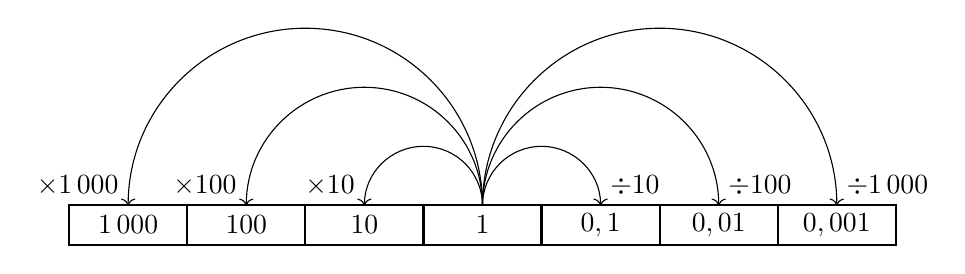
\begin{tikzpicture}[scale=0.5]
\foreach \x in {0,1,...,6} \draw[thick] (-1.5+3*\x,-0.5) rectangle (1.5+3*\x,0.5);
\draw (0,0) node {$1\,000$};
\draw (3,0) node {$100$};
\draw (6,0) node {$10$};
\draw (9,0) node {$1$};
\draw (12,0) node {$0,1$};
\draw (15,0) node {$0,01$};
\draw (18,0) node {$0,001$};
\draw[->] (9,0.5) arc (0:180:4.5) node[above left] {$\times 1\,000$};
\draw[->] (9,0.5) arc (0:180:3) node[above left] {$\times 100$};
\draw[->] (9,0.5) arc (0:180:1.5) node[above left] {$\times 10$};

\draw[->] (9,0.5) arc (180:0:4.5) node[above right] {$\div 1\,000$};
\draw[->] (9,0.5) arc (180:0:3) node[above right] {$\div 100$};
\draw[->] (9,0.5) arc (180:0:1.5) node[above right] {$\div 10$};
\end{tikzpicture}
\end{center}

Dans la partie entière $\left\lbrace
	\begin{matrix}
	\text{Une dizaine c'est l'unité prise 10 fois.}\\
	\text{Une centaine c'est l'unité prise 100 fois.}\\
	\text{Un millier c'est l'unité prise 1 000 fois.}\\
	\end{matrix}
\right.$ 

Dans la partie décimale $\left\lbrace
	\begin{matrix}
	\text{Une dixième c'est l'unité divisée par 10. Cela peut s'écrire} \frac{1}{10}. \\
	\text{Un centième c'est l'unité divisée par 100. Cela peut s'écrire} \frac{1}{100}. \\
	\text{Un millième c'est l'unité divisée par 1 000. Cela peut s'écrire} \frac{1}{1000}.
	\end{matrix}
\right.$

		\subsection{Ecriture fractionnaire d'un nombre}
\begin{aconnaitre}
Le "partage" de l'unité peut s'écrire \textbf{sous forme fractionnaire}.

Ainsi $\frac{1}{5}$ se lit "un cinquième". Cette fraction représente l'unité divisée en 5 parts égales. \\

\begin{center}
\begin{tikzpicture}[scale=0.5]
\fill[white] (0,0) rectangle (5,5);        % Specify colour
\fill[gray!40] (0,0) rectangle (1,5);        % Specify colour
\draw[thick] (0,0) -- (5,0) -- (5,5) -- (0,5) -- cycle;
\foreach \x in {1,2,3,4} \draw[thick] (\x,0) -- (\x,5);

\draw (2.5,0) node[below] {$\dfrac{1}{5}=0,2$};
\end{tikzpicture}
\end{center}

$\frac{1}{5}$ est \textbf{l'écriture fractionnaire} alors que 0,2 est \textbf{l'écriture décimale} \underline{d'une même quantité}.
\end{aconnaitre}

\begin{methode*1}[Comprendre les fractions]
	\begin{exemple*1}
\vspace{0.5cm}	
	
Dans le nombre $\frac{3}{5}$ l'unité est divisée en 5 parts égales et on a pris trois parts: $3\times \frac{1}{5}$.
\begin{center}
\begin{tikzpicture}[scale=0.5]
\fill[white] (0,0) rectangle (5,5);        % Specify colour
\fill[gray!40] (0,0) rectangle (3,5);        % Specify colour
\draw[thick] (0,0) -- (5,0) -- (5,5) -- (0,5) -- cycle;
\foreach \x in {1,2,3,4} \draw[thick] (\x,0) -- (\x,5);

\draw (2.5,0) node[below] {$\dfrac{3}{5}=0,6$};
\end{tikzpicture}
\end{center}

Le nombre du bas, celui qui indique le nombre de parts dans l'unité, s'appelle \textbf{\textcolor{C2}{le dénominateur}}.\\
Le nombre du haut, celui qui indique le nombre de parts, s'appelle \textbf{\textcolor{C2}{le numérateur}}.
\end{exemple*1}

\exercice

Dans chaque cas, donner l'écriture décimale correspondante:

$\frac{1}{100}$=\dotfill \\
$\frac{3}{4}$=\dotfill \\
$\frac{7}{10}$=\dotfill \\
$\frac{12}{25}$=\dotfill \\
$\frac{23}{50}$=\dotfill

\exercice

Dans chaque cas, donner une écriture fractionnaire correspondante:

0,5=\dotfill \\
0,32=\dotfill \\
0,04=\dotfill \\
0,25=\dotfill

\end{methode*1}

\begin{remarque}
Il est important de savoir calculer avec des écritures fractionnaires car certaines quantités ne peuvent pas s'écrire sous forme décimale.\end{remarque}

		\subsection{Partie entière et nombres en écriture fractionnaire}

Parfois, il arrive qu'on "garde" tellement de morceaux d'unité, qu'on arrive à reconstituer une ou plusieurs unités.

\begin{methode*1}[Fraction supérieure à 1]
	\begin{exemple*1}
\vspace{0.5cm}	
	
Prenons la fraction: $\frac{12}{5}$.\\
Cela signifie qu'on a gardé 12 parts égales à $\frac{1}{5}$.\\
Avec 5 parts égales à $\frac{1}{5}$, on peut faire une unité. Donc avec 12 parts de $\frac{1}{5}$, on peut constituer 2 unités et il restera 2 parts de $\frac{1}{5}$ c'est à dire $\frac{2}{5}$.\\
On peut donc dire que $\frac{12}{5}$=2+$\frac{2}{5}$=2,4.

\begin{center}
\begin{tikzpicture}[scale=0.5]
\fill[white] (0,0) rectangle (5,5);        % Specify colour
\fill[gray!40] (0,0) rectangle (5,5);        % Specify colour
\draw[thick] (0,0) -- (5,0) -- (5,5) -- (0,5) -- cycle;
\foreach \x in {1,2,3,4} \draw[thick] (\x,0) -- (\x,5);

\fill[white] (6,0) rectangle (11,5);        % Specify colour
\fill[gray!40] (6,0) rectangle (11,5);        % Specify colour
\draw[thick] (6,0) -- (11,0) -- (11,5) -- (6,5) -- cycle;
\foreach \x in {1,2,3,4} \draw[thick] (6+\x,0) -- (6+\x,5);

\fill[white] (12,0) rectangle (17,5);        % Specify colour
\fill[gray!40] (12,0) rectangle (14,5);        % Specify colour
\draw[thick] (12,0) -- (17,0) -- (17,5) -- (12,5) -- cycle;
\foreach \x in {1,2,3,4} \draw[thick] (12+\x,0) -- (12+\x,5);

\draw (8.5,0) node[below] {$\dfrac{12}{5}=2,4$};
\end{tikzpicture}
\end{center}

\end{exemple*1}

\exercice

Dans chaque cas, écrire la fraction sous forme d'une somme d'un entier et d'une autre fraction inférieure à 1 puis sous la forme d'un nombre décimal.

$\frac{6}{4}$=1+$\frac{2}{4}$=1,5\\
$\frac{9}{2}$=\dotfill \\
$\frac{35}{10}$=\dotfill \\
$\frac{17}{5}$=\dotfill \\
$\frac{143}{100}$=\dotfill

\end{methode*1}

%%%%%%%%%%%%%%%%%%%%%%%%%%%%%%%%%%%%%%%%%%%%%%%%%%%%%%%%%%%%%%%%%%%%%%%%%%%

\section{Droite ou axe gradué}

\begin{aconnaitre}
Les \textbf{\textcolor{C2}{nombres entiers}}
peuvent être placés sur une droite ou un axe. A chaque point de la droite, on associe un nombre: c'est l'abscisse du point.
\end{aconnaitre}
\begin{methode*1}[Repérer sur une demi-droite graduée]
	\begin{exemple*1}

\vspace{0.5cm}

 
 L'abscisse du point $F$ est $\frac{1}{5}=0,2$ donc on note F(0,2).
 
 L'abscissedu point $G$ est $\frac{6}{5}=6 \times0,2=1,2$ donc on note G(1,2).
 
 L'abscisse du point $H$ est $\frac{11}{5}=11 \times0,2=2,2$ donc on note H(2,2).
   
 
\tikzset{
   cross/.pic = {
     \draw[thick] (-0.2,0.2) -- (0.2,-0.2);
     \draw[thick] (-0.2,-0.2) -- (0.2,0.2);}
}

\begin{tikzpicture}[general]
% The axis
\draw[decoration={markings,mark=at position 1 with
    {\arrow[scale=3]{>}}},postaction={decorate}] (0,0) -- (12,0); 
% The ticks
\foreach \x in {0,...,11} \draw (\x,-0.2) -- (\x,0.2);
\foreach \x in {0,1,2} \draw (5*\x,-0.35) -- (5*\x,0.35);
% The numbers
\draw (0,-0.35) node[below] {\large $0$};
\draw (5,-0.35) node[below] {\large $1$};
% The markers
\pic[scale=0.6] at (1,0) {cross}; \draw (1,0.5) node {\large $F$};
\pic[scale=0.6] at (6,0) {cross}; \draw (6,0.5) node {\large $G$};
\pic[scale=0.6] at (11,0) {cross}; \draw (11,0.5) node {\large $H$};
\end{tikzpicture}
\end{exemple*1}

\begin{remarque}
Il arrive parfois que les graduations de l'axe ne commencent pas à 0 ou que l'axe ne soit pas gradué de 1 en 1. Dans ce cas, il s'agit de repérer la valeur d'\textbf{une} graduation grâce aux valeurs données.
\end{remarque}

\exercice

\tikzset{
   cross/.pic = {
     \draw[thick] (-0.2,0.2) -- (0.2,-0.2);
     \draw[thick] (-0.2,-0.2) -- (0.2,0.2);}
}

\begin{tikzpicture}[general]
% The axis
\draw[decoration={markings,mark=at position 1 with
    {\arrow[scale=3]{>}}},postaction={decorate}] (-0.8,0) -- (11.5,0); 
% The ticks
\foreach \x in {1,...,11} \draw (0.8*\x,-0.2) -- (0.8*\x,0.2);
\foreach \x in {0,1,...,6} \draw (0.8*2*\x,-0.35) -- (0.8*2*\x,0.35);
% The numbers
%\draw (0,-0.35) node[below] {\large $0$};
%\draw (5,-0.35) node[below] {\large $50$};
% The markers
\pic[scale=0.6] at (0,0) {cross}; \draw (0,0.5) node {\large $P$};
\pic[scale=0.6] at (0.8*5,0) {cross}; \draw (0.8*5,0.5) node {\large $S$};
%\pic[scale=0.6] at (0.8*8,0) {cross}; 
\draw (0.8*8,-0.6) node {\large $800$};
\draw (0.8*12,-0.6) node {\large $1\,000$};
\pic[scale=0.6] at (0.8*13,0) {cross};  \draw (0.8*13,0.5) node {\large $R$};
\end{tikzpicture}

Ici, de 800 à 1000, il y a \dotfill graduations. Donc chaque graduation représente \dotfill .

L'abscisse du point \dotfill est \dotfill donc on note \dotfill. 

L'abscisse du point \dotfill est \dotfill donc on note \dotfill. 

L'abscisse du point \dotfill est \dotfill donc on note \dotfill. 
\end{methode*1}

%%%%%%%%%%%%%%%%%%%%%%%%%%%%%%%%%%%%%%%%%%%%%%%%%%%%%%%%%%%%%%%%%%%%%%%%%%%
\section{Travail sur les nombres: encadrer et arrondir}

% remarque : pour qu'un mot se retrouve dans le lexique : \MotDefinition{asymptote horizontale}{} 


\begin{aconnaitre}
\textbf{\MotDefinition{Encadrer}{}} un nombre, c'est trouver un nombre qui est plus petit que lui et un nombre qui est plus grand que lui. On écrit un encadrement avec les symboles $<$ ; $\leqslant$ ; $>$ et $\geqslant$. 
\end{aconnaitre}


\begin{methode*1}[Encadrer]

\begin{exemple*1}
Encadrer 13,345 à l'unité puis au centième.\\[0.5em]
Pour encadrer à l'unité, on «coupe» le nombre 13,345 à l'unité: 13.\
13 est plus petit  que 13,345 qui est plus petit que 14 (on ajoute une \textbf{unité}) .\
On écrit alors : $13 < 13,345 < 14$. \\[1em]
Pour encadrer au centième, on «coupe» le nombre 13,345 au centième: 13,34.\
13,34 est plus petit que 13,345 qui est plus grand que 13,35 (on ajoute un \textbf{centième}).\
On écrit alors : $13,34 < 13,345 < 13,35$.
\end{exemple*1}

\exercice

Encadrer les nombres 237,48 et 43,923\,5 à la dizaine puis au centième.
%\correction

\end{methode*1}

%%%%%%%%%%%%%%%%%%%%%%%%%%%%%%%%%%%%%%%%%%%%%%%%%%%%%%%%%%%%%%%%%%%%%%%%%%


\begin{aconnaitre}
\textbf{\MotDefinition{Arrondir}{}} un nombre, c’est le remplacer par le nombre le plus proche à la précision désirée. Pour cela:
\begin{itemize}
 \item on encadre le nombre à la précision demandée ;
 \item on choisit la valeur (inférieure ou supérieure) qui est la plus proche du nombre d'origine.
 \end{itemize}


On peut aussi regarder comment le nombre est formée:
\begin{itemize}
\item on choisit le dernier chiffre à conserver;
 \item on conserve ce chiffre si le suivant est 0, 1, 2, 3 ou 4 ;
 \item on augmente de 1 ce chiffre si le suivant est 5, 6, 7, 8, ou 9.
 \end{itemize}
\end{aconnaitre}


\begin{methode*1}[Arrondir]

\begin{exemple*1}
Donner l'arrondi \textbf{à l'unité} de 73,2.\\
%%%%%%%%%%%%%Illustration Paul
Donner l'arrondi \textbf{à l'unité} de 126,5.\\
%%%%%%%%%%%%%Illustration Paul
Donner l'arrondi \textbf{au centième} de 2,396.\\
%%%%%%%%%%%%%Illustration Paul
Donner l'arrondi \textbf{au centième} de 12,543.\\
%%%%%%%%%%%%%Illustration Paul

\end{exemple*1}

\exercice

Arrondir à l'unité les nombres 1247,20 et 25,385. Arrondir au dixième les nombres 1,99 et 3,14159.

%\correction

\end{methode*1}


\exercicesbase
\begin{colonne*exercice}
 \definecolor{fondTI}{HTML}{869286}


\serie{Les nombres entiers}

\begin{exercice}[Un peu de vocabulaire]
Recopie et complète les phrases suivantes afin de les rendre exactes :
\begin{enumerate}
 \item Un \ldots \ldots \ldots est composé de chiffres ;
 \item 9 est un \ldots \ldots \ldots composé d'un seul \ldots \ldots \ldots ;
 \item Le chiffre des centaines du nombre 2\,568 est \ldots \ldots ;
 \item 3 est le chiffre des \ldots \ldots \ldots du nombre 783 ;
 \item \ldots \ldots est le chiffre des milliers du nombre 120\,452 ;
 \item Le chiffre des \ldots \ldots \ldots du nombre 43 est 4.
\end{enumerate}
\end{exercice}

\begin{exercice}
Écris en chiffres les nombres suivants :
\begin{enumerate}
 \item Sept mille huit cent douze ;
 \item Soixante-trois mille neuf cent cinquante ;
 \item Huit millions trois ;
 \item Septante-quatre milliards cent quatre ;
 \item Cent trente-six millions huit cent nonante-trois mille sept cent cinq.
 \end{enumerate}
\end{exercice}

\begin{exercice}
Classe les nombres suivants dans l'ordre décroissant (du plus grand au plus petit) :
\begin{colitemize}{2}
 \item 23\,100 ;
 \item Cent vingt-trois mille ;
 \item 1\,320 ;
 \item Mille cent vingt-trois.
 \end{colitemize}
\end{exercice}

%%%%%%%%%%%%%%%%%%%%%%%%%%%%%%%%%%%%%%%%%%%%%%%%%%%%%%%%%%%%%%%%%%%%%%%%%%%

\serie{Les nombres décimaux}

\begin{exercice}[Dans un sens]
Donne l'écriture décimale :
\begin{enumerate} 
 \item 75 milliers \dotfill ; 

 \item 5 centièmes \dotfill ; 

 \item 13 dizaines \dotfill ; 

 \item 9 dixièmes \dotfill ; 

 \item 35 centaines \dotfill ;

 \item 956 millièmes \dotfill. 

 \end{enumerate}
\end{exercice}


\begin{exercice}[Décomposition]
Donne une écriture décimale qui correspond à chacune des décompositions suivantes :
\begin{enumerate}
 \item $(3 \cdot 10) + (4 \cdot 1) + (4 \cdot 0,1) + (7 \cdot 0,01)$
 \item $(8 \cdot 100) + (5 \cdot 1) + (9 \cdot 0,1) + (6 \cdot 0,01)$
 \item $(5 \cdot 1) + (4 \cdot 0,01) + (3 \cdot 0,001)$
 \item $(7 \cdot 100) + (9 \cdot 1) + (8 \cdot 0,1) + (6 \cdot 0,001)$
 \end{enumerate}
\end{exercice}


\begin{exercice}[Décomposition (bis)]
Décompose chacun de ces nombres de la même façon qu'à l'exercice précédent :
\begin{enumerate} 
 \item 9,6 \dotfill ; 
 
 \item 84,258 \dotfill ; 
 
 \item 7,102 \dotfill ;
 
 \item 123,015 \dotfill ; 
 
 \item 0,008\,3 \dotfill ; 
 
 \item 1\,002,200\,4 \dotfill.
 
 \end{enumerate}
\end{exercice}

\begin{exercice}[Combien de \ldots dans \ldots ?]
\begin{enumerate}
 \item Combien de millièmes y a-t-il dans une unité ?
Traduis cela par une égalité mathématique.
 \item Combien de centièmes y a-t-il dans une unité ? Traduis cela par une égalité mathématique.
 \item Combien de centièmes y a-t-il dans un dixième d'unité ? Traduis cela par une égalité mathématique.
 \end{enumerate}
\end{exercice}


\begin{exercice}
Complète les égalités :
\begin{enumerate}
 \item 4 unités 6 dixièmes = \ldots \ldots dixièmes ;
 \item  \ldots \ldots  unité \ldots \ldots centièmes = 123 centièmes ;
 \item 12 unités 37 millièmes = \ldots \ldots millièmes.
 \end{enumerate}
\end{exercice}


\begin{exercice}
Donne une écriture décimale des nombres suivants :
\begin{enumerate}
 \item Sept unités et huit dixièmes \dotfill ;
 \item Cent unités, huit dixièmes et un centième
 
 \dotfill ;
 \item Deux unités et trois centièmes
 
 \dotfill ;
 \item Treize centaines \dotfill ;
 \item Trente-six milliers et huit millièmes
 
 \dotfill ;
 \item Cinq unités et quinze millièmes \dotfill.
 \end{enumerate}
\end{exercice}


\begin{exercice}[Vocabulaire des nombres décimaux]
\begin{enumerate}
 \item Quel est le chiffre des millièmes de 24,738 ?
 
 \dotfill ;
 \item Quel est le nombre de millièmes de 24,738 ?
 
 \dotfill ;
 \item Que représente le chiffre 3 dans 7\,859,342 ?
 
 \dotfill ;
 \item Quel est le nombre de centièmes de 17,78 ?
 
 \dotfill ;
 \item Quel est le chiffre des centièmes de 71,865 ?
 
 \dotfill ;
 \item Donne la partie entière du nombre 83,712 :
 
 \dotfill ;
 \item Donne la partie décimale du nombre 54,91 :
 
 \dotfill.
 \end{enumerate}
\end{exercice}


\begin{exercice}
Trouve un nombre à cinq chiffres ayant 7 pour chiffre des dizaines, 9 pour chiffre des centièmes, 0 pour chiffre des unités, 3 pour chiffre des millièmes et comme autre chiffre 1.
\end{exercice}


\begin{exercice}[Devinette]
Trouve le nombre ayant les caractéristiques suivantes :
\begin{itemize}
 \item il n'a que deux chiffres après la virgule ;
 \item il a la même partie entière que 1 890,893 ;
 \item son chiffre des centièmes est le même que celui de 320,815 ;
 \item son chiffre des dixièmes est égal à la moitié de celui de 798,635.
 \end{itemize}
\end{exercice}


\begin{exercice}[Zéros inutiles]
Écris, lorsque cela est possible, les nombres suivants avec moins de chiffres.
\begin{enumerate} 
 \item 17,200 \dotfill ; 
 
 \item 123,201 \dotfill ; 
  
 \item 36,700\,10 \dotfill ; 
 
 \item 0\,021,125 \dotfill ; 
 
 \item 0,123\,0 \dotfill ; 
 
 \item 023,201\,20 \dotfill ; 
 
 \item 30,000 \dotfill ; 
 
 \item 0\,050,12 \dotfill ; 
 
 \item 1\,205\,500,0 \dotfill. 
  
 \end{enumerate}
\end{exercice}

\begin{exercice}[« Chiffre des » ou « nombre de »]
\begin{enumerate}
 \item Recopie et complète les phrases suivantes afin de les rendre exactes :
 \begin{itemize}
  \item $127 = 12 \cdot \ldots + 7$:
  
  127 possède donc \ldots \ldots dizaines ;
  \item $841\,123 = 841 \cdot \ldots + \ldots \ldots$ :
  
  841\,123 possède donc 841 \ldots \ldots ;
  \item $3\,816 = \ldots \cdot 100 + \ldots \ldots$ :
  
  \ldots \ldots possède donc \ldots \ldots .
  \end{itemize}
 \item Dans le nombre entier 15, quel est le nombre d'unités ? Le chiffre des unités ?
 \item Combien y a-t-il de centaines dans 4\,125 ?
 \item Quel est le chiffre des dizaines dans le nombre entier 498 ? Et le nombre de dizaines ?
 \item Dans 25 dizaines, quel est le nombre d'unités ?
 \end{enumerate}
\end{exercice}


\begin{exercice}
Donne l'écriture en chiffres des nombres entiers suivants :
\begin{enumerate}
 \item $(9 \cdot 10) + 5$ ;
 \item $(7 \cdot 1\,000) + (5 \cdot 100) + (2 \cdot 10) + 8$ ;
 \item $(1 \cdot 10\,000) + (1 \cdot 100) + 1$ ;
 \item  $(3 \cdot 100\,000) + (7 \cdot 10\,000) + (4 \cdot 10) + 9$ ;
 \item  $(3 \cdot 100\,000) + (4 \cdot 100) + (7 \cdot 1\,000) + 9$.
 \end{enumerate}
\end{exercice}


\begin{exercice}[Sur une demi-droite graduée]
Donne les abscisses des points $A$, $B$ et $C$, sous la forme d'un nombre décimal.
\begin{center} \includegraphics[width=7cm]{axe0AB1C} \end{center}
\end{exercice}


\begin{exercice}
Sur la demi-droite graduée ci-dessous, place les points $O(0)$, $A(1)$, $B(2)$, $C(0,5)$, $D(1,6)$, $E(0,1 + 0,05)$, $F(0,2)$, $G(1 + 0,05)$ et $H(1,45)$ :
\begin{center} \includegraphics[width=7cm]{axe012x} \end{center}
\end{exercice}

%%%%%%%%%%%%%%%%%%%%%%%%%%%%%%%%%%%%%%%%%%%%%%%%%%%%%%%%%%%%%%%%%%%%%%%%%%%

\serie{Comparaison}

\begin{exercice}[Demi-droite graduée et comparaison]
\begin{enumerate}
 \item Reproduis la demi-droite graduée suivante et place les points $A(7,39)$ ; $B(7,46)$ et $C(7,425)$ :
\begin{center} \includegraphics[width=6.6cm]{axe74E-75D} \end{center}
 \item Range dans l'ordre décroissant les abscisses de tous les points qui sont nommés.
 \end{enumerate}
\end{exercice}

\begin{exercice}[Rangement]
Range les nombres suivants dans l'ordre croissant :

5 ; 4,99 ; 4,9 ; 4,88 ; 5,000 1 ; 4,909 ; 4,879 :

\dotfill

\dotfill
\end{exercice}


\begin{exercice}[Rangement $(bis)$]
Range les nombres suivants dans l'ordre décroissant :

120 ; 119,999 ; 120,000 1 ; 120,101 ; 119,9 ; 119 ; 119,990 9 ; 120,100 1 ; 102,01 ; 120,1 :

\dotfill

\dotfill
\end{exercice}

%%%%%%%%%%%%%%%%%%%%%%%%%%%%%%%%%%%%%%%%%%%%%%%%%%%%%%%%%%%%%%%%%%%%%%%%%%%
\serie{Encadrer}


\begin{exercice}[Encadrer à la dizaine]
235,5 ; 45 ; 1270 ; 574,23 ; 10\,095.
\end{exercice}


\begin{exercice}[Encadrer au dixième]
76,123 ; 461,99 ; 1\,254,01 ; 3,93 ; 9,99.
\end{exercice}



\begin{exercice}
Dans chaque cas, propose, si cela est possible, un nombre entier que l'on peut intercaler entre les deux nombres donnés. 
Y a‑t‑il plusieurs solutions ? Si oui, cite‑les :
\begin{enumerate}
 \item $5 < …… < 6$ ;
 \item $6,4 < …… < 6,8$ ;
 \item $3,8 < …… < 5,3$ ;
 \item $6,5 < …… < 7,21$.
 \end{enumerate}
\end{exercice}


\begin{exercice}
Dans chaque cas, donne trois exemples différents de nombres décimaux que l'on peut intercaler entre les deux nombres donnés :
\begin{enumerate}
 \item $6 < …… < 7$ ;
 \item $4,5 < …… < 4,9$ ;
 \item $3,45 < …… < 3,48$ ;
 \item $6,8 < …… < 6,9$ ;
 \item $15,13 < …… < 15,14$ ;
 \item $3,238 < …… < 3,24$.
 \end{enumerate}
\end{exercice}


\begin{exercice}[Chiffres masqués]
Certains chiffres sont masqués par \#. Lorsque cela est possible, complète les pointillés avec $<$,$>$ ou $=$ :
\begin{enumerate} 
 \item $6,51 …… 6,7\#$ ;
 \item $5,42 …… 5,0\#$ ;
 \item $\#,23 …… 4,16$ ;
 \item $6,04 …… 6,1\#$ ;
 \item $3,\#35 …… 3,01$ ;
 \item $43,\#96 …… 43,0\#$.
 \end{enumerate}
\end{exercice}


\begin{exercice}[Nombres à trouver]
Dans chaque cas, complète les pointillés par un nombre décimal :
\begin{enumerate} 
 \item $24,5 < ...... < 24,6$ ;  
 
 \item $12,99 < ...... < 13$ ; 
 
 \item $32,53 < ...... < 32,54$ ; 
 
 \item $58 < ...... < 58,01$ ; 
 
 \item $5,879 < ...... < ...... < ...... < 5,88$. 

 \end{enumerate}
\end{exercice}

%%%%%%%%%%%%%%%%%%%%%%%%%%%%%%%%%%%%%%%%%%%%%%%%%%%%%%%%%%%%%%%%%%%%%%%%%%%
\serie{Arrondir}

\begin{exercice}[Arrondir à l'unité]
Arrondis à l'unité les nombres suivants :
\begin{enumerate}
 \item 46,8 \dotfill ; 
 
 \item 109,75 \dotfill ; 
 
 \item 1,3 \dotfill ; 
 
 \item 0,09 \dotfill ; 
 
 \item 234,08 \dotfill ; 
 
 \item 4\,087,63 \dotfill. 
 
 \end{enumerate}
\end{exercice}


\begin{exercice}[Arrondir à la dizaine]
Arrondis à la dizaine les nombres suivants :
\begin{enumerate}
 \item 234,2 \dotfill ; 
 
 \item 3,14 \dotfill ; 
 
 \item 17,62 \dotfill ; 
 
 \item 889,3 \dotfill ; 
 
 \item 6\,289,3 \dotfill ; 
 
 \item 23,005 \dotfill. 
 
 \end{enumerate}
\end{exercice}


\begin{exercice}[Arrondir au dixième]
Arrondis au dixième les nombres suivants :
\begin{enumerate}
 \item 8,372 \dotfill ; 
 
 \item 50,64 \dotfill ; 
 
 \item 30,18 \dotfill ; 
 
 \item 43,725 \dotfill ; 
 
 \item 0,02 \dotfill ; 
 
 \item 78,66 \dotfill. 
 
 \end{enumerate}
\end{exercice}


%%%%%%%%%%%%%%%%%%%%%%%%%%%%%%%%%%%%%%%%%%%%%%%%%%%%%%%%%%%%%%%%%%%%%%%%%%%



\end{colonne*exercice}


\exercicesappr
\begin{colonne*exercice}
\begin{exercice}[Nombres croisés]
Recopie et complète la grille à l'aide des nombres que tu trouveras grâce aux définitions :

\begin{center}
\begin{tabularx}{.5\linewidth}{r|c|c|c|c|c|}
\multicolumn{1}{c}{}& \multicolumn{1}{c}{\textbf{A}} & \multicolumn{1}{c}{\textbf{B}} & \multicolumn{1}{c}{\textbf{C}} & \multicolumn{1}{c}{\textbf{D}} & \multicolumn{1}{c}{\textbf{E}} \\ \cline{2-6}
\textbf{I} & & & & \cellcolor{black} & \\ \cline{2-6} 
\textbf{II} & & & & & \\ \cline{2-6} 
\textbf{III} & & \cellcolor{black} & & & \\ \cline{2-6} 
\textbf{IV} & & & & & \cellcolor{black} \\ \cline{2-6} 
\textbf{V} & \cellcolor{black} & & & & \\ \cline{2-6} 
\end{tabularx}
\end{center}

\vspace{0.75em}

\textbf{Horizontalement}

\textbf{I} : La partie entière de 328,54. Le chiffre des centièmes de 634,152.

\textbf{II} : Son chiffre des dizaines est le triple de celui des unités.

\textbf{III} : Le chiffre des dixièmes de 34. Arrondi à l'unité de 178,356.

\textbf{IV} : Entier compris entre 8\,000 et 9\,000.

\textbf{V} : Quarante-deux centaines.

\vspace{0.75em}

\textbf{Verticalement}

\textbf{A} : $(3 \times 1 000) + (5 \times 100) + (8 \times 1)$.

\textbf{B} : Le nombre de dixièmes dans 2,6. La partie entière de 2\,498 centièmes.

\textbf{C} : Quatre-vingt-six milliers et cent deux unités.

\textbf{D} : En additionnant tous les chiffres de ce nombre, on trouve 20.

\textbf{E} : Arrondi à l'unité de 536,57. Entier qui précède 1.

\end{exercice}


\begin{exercice}
Voici les résultats (en secondes), pour les hommes, du 100 m aux JO de Pékin en 2008 : \vspace{0.75em}

Martina : 9,93 ; Frater : 9,97 ; Burns : 10,01 ; Patton : 10,03 ; Bolt : 9,69 ; Powell : 9,95 ; Thompson : 9,89 ; Dix : 9,91.\vspace{0.75em}

Classe les coureurs dans l'ordre décroissant de leur résultat.
\end{exercice}


\begin{exercice}[À ordonner]
Range les nombres suivants dans l'ordre croissant : \vspace{0.75em}

25 unités et deux dixièmes ; 2\,504 centièmes; $25 + 2$ centièmes ; deux mille cinquante‑deux centièmes ; 20,54 ; 254 dixièmes.
\end{exercice}


\begin{exercice}[À placer]
En choisissant judicieusement la longueur d'une graduation, place précisément sur une demi‑droite graduée les points $A$, $B$, $C$, $D$ et $E$ d'abscisses respectives : \\[0.75em]
12,02 ; mille deux cent treize centièmes ; $12 + 7$ centièmes ; 1\,198 centièmes ; cent vingt-et-un dixièmes.
\end{exercice}


\begin{exercice}[Comparaison]
\begin{enumerate}
 \item Quel est le plus grand nombre décimal ayant un chiffre après la virgule et inférieur à 83 ?
 \item Quel est le plus petit nombre décimal avec trois chiffres après la virgule et supérieur à 214,3 ?
 \item Quel est le plus grand nombre décimal avec deux chiffres après la virgule, ayant tous ses chiffres différents et qui est inférieur à 97,8 ?
 \item Quel est le plus petit nombre décimal avec trois chiffres après la virgule, ayant tous ses chiffres différents et qui est supérieur à 2\,341 ?
 \end{enumerate}
\end{exercice}


\begin{exercice} 
Voici les masses de lipides et glucides (en g) contenues dans 50 g de différents biscuits :

\begin{center}
\begin{tabularx}{\linewidth}{|c|*{6}{>{\centering \arraybackslash}X|}}
\hline \rowcolor{U1} Biscuit & A & B & C & D & E \\
\hline \cellcolor{U1} Lipides & 9,527 & 9,514 & 9,53 & 9,521 & 9,6 \\
\hline \cellcolor{U1} Glucides & 32,43 & 33 & 33,6 & 33,15 & 33,50 \\
\hline
\end{tabularx} \\
\end{center}

\begin{enumerate}
 \item Classe ces biscuits selon l'ordre croissant de leur quantité de lipides ;
 \item Classe ces biscuits selon l'ordre décroissant de leur quantité de glucides.
 \end{enumerate}
\end{exercice}


\begin{exercice}[Énigme]
Trouve le nombre décimal à six chiffres tel que :
\begin{itemize}
 \item son chiffre des unités est 2 ;
 \item l'un de ses chiffres est 6 et sa valeur dans l'écriture décimale est cent fois plus petite que celle du chiffre 2 ;
 \item son chiffre des dizaines est le double de celui des unités et son chiffre des dixièmes est le quart de celui des dizaines ;
 \item ce nombre est compris entre 8\,975,06 et 9\,824,95 ;
 \item la somme de tous ses chiffres est égale à 27.
 \end{itemize}
\end{exercice}
\end{colonne*exercice}





%\themaC
%\chapter{Opérations avec les nombres décimaux}\label{ChOpNbEntDec}

\begin{acquis}
\begin{itemize}
\item multiplier et diviser mentalement par 0,1; 0,01; 0,001; 10; 100; 1 000… des nombres décimaux et compléter les opérations à trous correspondantes;
\item soustraire, additionner et multiplier des nombres décimaux;
\item faire une division décimale par un diviseur entier et non entier avec un résultat exact ou un résultat à une précision donnée ou un résultat arrondi;
\item résoudre des problèmes dont la solution conduit à effectuer 2 ou 3 opérations successives parmi l’addition, la soustraction, la multiplication et la division de décimaux;
\item utiliser le vocabulaire suivant : somme, différence, produit, quotient, terme, facteur, dividende, diviseur et reste;
\end{itemize}
\end{acquis}

\cours
\section{Multiplier/diviser un nombre décimal par 10, 100, 1000}
%%%%%%%%%%%%%%%%%%%%%%%%%%%%%%%%%%%%%%%%%%%%%%%%%%%%%%%%%%%%%%%%%%%%%%%%%%%
\prof
{En primaire et de façon usuelle, on a l'habitude de parler de virgule qui se déplace. Cependant, pour coller à la réalité mathématiques, on préférera ici parler de quantité qui augment ou qui diminue et donc de chiffres qui se déplacent. Cela n'empêche pas, une fois le concept acquis de montrer qu'on peut imaginer un déplacement de la virgule.}
%%%%%%%%%%%%%%%%%%%%%%%%%%%%%%%%%%%%%%%%%%%%%%%%%%%%%%%%%%%%%%%%%%%%%%%%%%%

\begin{aconnaitre}

\hspace{2em}\textbullet\hspace{.25em} Multiplier un nombre décimal par 10, 100 ou 1 000 revient à \textbf{\textcolor{C2}{déplacer chacun de ses chiffres vers la gauche}} de 1, 2 ou 3 rangs pour lui donner une valeur 10, 100 ou 1 000 fois plus grande.

\hspace{2em}\textbullet\hspace{.25em} Diviser un nombre décimal par 10, 100 ou 1 000 revient à \textbf{\textcolor{C2}{déplacer chacun de ses chiffres vers la droite}} de 1, 2 ou 3 rangs pour lui donner une valeur 10, 100 ou 1 000 fois plus petite.

\end{aconnaitre}

\begin{methode*1}[]
	\begin{remarque}
On devra parfois ajouter des zéros dans l'écriture.
	\end{remarque}
	\begin{exemple*1}

Effectuer les calculs $6,5 \div 100$ et $0,47 \times 1000$ [0.5em]

\begin{minipage}{.4\linewidth}
\begin{ttableau}{.8\linewidth}{4}
\hline
 \rotatebox{90}{unités} & \rotatebox{90}{dixièmes} & \rotatebox{90}{centièmes\phantom{x}} & \rotatebox{90}{millièmes} \\ \hline
 \textcolor{B1}{\textbf{6}} , & \textcolor{B1}{\textbf{5}} & & \\ \hline
 $0\,,$ & 0 & \textcolor{B1}{\textbf{6}} & \textcolor{B1}{\textbf{5}} \\ \hline
\end{ttableau}
\end{minipage}\hfill%
%
\begin{minipage}{.55\linewidth}
Pour diviser 6,5 par \textcolor{B1}{\textbf{100}}, on déplace chacun de ses chiffres vers la droite de \textcolor{B1}{\textbf{2}} rangs et on ajoute les zéros nécessaires. 

On obtient $6,5 \div 100 = 0,065$.

\end{minipage}
%

\vspace{2em}

\begin{minipage}{.4\linewidth}
\begin{ttableau}{\linewidth}{5}
\hline
\rotatebox{90}{centaines} & \rotatebox{90}{dixaines} & \rotatebox{90}{unités} & \rotatebox{90}{dixièmes} & \rotatebox{90}{centièmes\phantom{x}} \\ \hline
 & & 0 , & \textcolor{J1}{\textbf{4}} & \textcolor{J1}{\textbf{7}} \\ \hline
 \textcolor{J1}{\textbf{4}} & \textcolor{J1}{\textbf{7}} & 0 & &\\ \hline
\end{ttableau}
\end{minipage}\hfill%
%
\begin{minipage}{.55\linewidth}
Pour multiplier 0,47 par \textcolor{J1}{\textbf{1\,000}}, on déplace chacun de ses chiffres vers la gauche de \textcolor{J1}{\textbf{3}} rangs et on ajoute les zéros nécessaires. 

On obtient $0,47 \times 1\,000 = 470$. 
\end{minipage}
	\end{exemple*1}
	
\exercice

Compléter par le signe qui convient.
\begin{colenumerate}{4}
 \item $0,8 \dotfill 100=80$ ;
 \item $0,38 \dotfill 10=0,038$ ;
 \item $47 \dotfill 100=0,47$ ;
 \item $5 \dotfill 0,1=0,5$;
 \end{colenumerate}


\exercice

Effectue : 
\begin{colenumerate}{4}
 \item $3,6 \times 100$ ;
 \item $870 \times 1\,000$ ;
 \item $63 \div 10$ ;
 \item $87\,654 \div 100$.
 \end{colenumerate}
%\correction
 
\end{methode*1}








%%%%%%%%%%%%%%%%%%

\section{Multiplier/diviser un nombre décimal par 0,1 ; 0,01 ; 0,001}

\begin{aconnaitre}
\textbf{Multiplier} un nombre décimal par \textcolor{A1}{\textbf{0,1}}, \textcolor{B1}{\textbf{0,01}} ou \textcolor{J1}{\textbf{0,001}} revient à déplacer chacun de ses chiffres vers \textbf{la droite} de 1, 2 ou \textcolor{J1}{\textbf{3}} rangs pour lui donner une valeur 10, 100 ou \textcolor{J1}{\textbf{1\,000}} fois plus petite.
\textbf{Diviser} un nombre décimal par \textcolor{A1}{\textbf{0,1}}, \textcolor{B1}{\textbf{0,01}} ou \textcolor{J1}{\textbf{0,001}} revient à déplacer chacun de ses chiffres vers \textbf{la gauche} de \textcolor{A1}{\textbf{1}}, \textcolor{B1}{\textbf{2}} ou \textcolor{J1}{\textbf{3}} rangs pour lui donner une valeur \textcolor{A1}{\textbf{10}}, \textcolor{B1}{\textbf{100}} ou \textcolor{J1}{\textbf{1\,000}} fois plus grande.
\end{aconnaitre}


\begin{methode*1}[Multiplier ou diviser un nombre décimal par 0,1 ; 0,01 ; 0,001 \ldots]

\begin{remarque}
On devra parfois ajouter des zéros dans l'écriture.
\end{remarque}

\begin{exemple*1}
Effectue les calculs $2,5 \times 0,01$ et $0,65 \div 0,001$.\\[1em]

\begin{minipage}{.4\linewidth}
\begin{ttableau}{.8\linewidth}{4}
\hline
 \rotatebox{90}{unités} & \rotatebox{90}{dixièmes} & \rotatebox{90}{centièmes\phantom{x}} & \rotatebox{90}{millièmes} \\ \hline
 \textcolor{B1}{\textbf{2}} , & \textcolor{B1}{\textbf{5}} & & \\ \hline
 $0\,,$ & 0 & \textcolor{B1}{\textbf{2}} & \textcolor{B1}{\textbf{5}} \\ \hline
\end{ttableau}
\end{minipage}\hfill%
%
\begin{minipage}{.55\linewidth}
Pour multiplier 2,5 par \textcolor{B1}{\textbf{0,01}}, on déplace chacun de ses chiffres vers la droite de \textcolor{B1}{\textbf{2}} rangs et on ajoute les zéros nécessaires. 

On obtient $2,5 \times 0,01 = 0,025$.
\end{minipage}
%

\vspace{2em}

%
\begin{minipage}{.4\linewidth}
\begin{ttableau}{\linewidth}{5}
\hline
\rotatebox{90}{centaines} & \rotatebox{90}{dixaines} & \rotatebox{90}{unités} & \rotatebox{90}{dixièmes} & \rotatebox{90}{centièmes\phantom{x}} \\ \hline
 & & 0 , & \textcolor{J1}{\textbf{6}} & \textcolor{J1}{\textbf{5}} \\ \hline
 \textcolor{J1}{\textbf{6}} & \textcolor{J1}{\textbf{5}} & 0 & &\\ \hline
\end{ttableau}
\end{minipage}\hfill%
%
\begin{minipage}{.55\linewidth}
Pour diviser 0,65 par \textcolor{J1}{\textbf{0,001}}, on déplace chacun de ses chiffres vers la gauche de \textcolor{J1}{\textbf{3}} rangs et on ajoute les zéros nécessaires. 

On obtient $0,65 \div 0,001 = 650$.
\end{minipage}
\end{exemple*1}


\exercice

Effectuer :
\begin{colenumerate}{4}
 \item $5,45 \times 0,1$ ;
 \item $854 \times 0,001$ ;
 \item $63 \div 0,1$ ;
 \item $87,54 \div 0,01$.
 \end{colenumerate}
%\correction

\end{methode*1}

%%%%%%%%%%%%%%%%%%%%%%%%%%%%%%%%%%%%%%%%%%%%%%%%%%%%%%%%
\section{Multiplication}
\begin{remarque}

Multiplier c'est répéter la même quantité un certain nombre de fois.
\end{remarque}
	\subsection{Multiplier des décimaux}
\begin{aconnaitre}
Le résultat d'une multiplication s'appelle un produit. Les nombres que l'on multiplie sont des facteurs.
\end{aconnaitre}

\begin{methode*1}[Multiplication]
\begin{exemple*1}

$12 \times 4=48$

48 est le produit. 12 et 4 sont des facteurs.
\end{exemple*1}

\exercice

$13\times 3=39$

\dotfill est le \dotfill . \dotfill et \dotfill sont des \dotfill .

\end{methode*1}

	\subsection{Multiplier plusieurs facteurs}
\begin{aconnaitre}
Dans le calcul d'un produit de plusieurs facteurs, on peut:

\hspace{2em}\textbullet\hspace{.25em} changer l'ordre des facteurs.

\hspace{2em}\textbullet\hspace{.25em} regrouper différemment certains facteurs pour faciliter les calculs.
\end{aconnaitre}
\begin{methode*1}[]
\begin{exemple*1}

$25 \times 32 \times 4=25 \times 4 \times 32=100  \times 32 = 3200$
\end{exemple*1}

\exercice

$2 \times 3 \times 5= \dotfill$
\end{methode*1}
	
	\subsection{Multiplier deux nombres décimaux}
\begin{methode*1}[Multiplication de décimaux]
\begin{exemple*1}

Effectue la multiplication de 2,34 par 1,2.\\[0.5em]

On pose l'opération comme s'il s'agissait de nombres entiers. 

On effectue la multiplication de 234 par 12 sans tenir compte des virgules.

\begin{minipage}{.6\linewidth}
\begin{tabular}{rrrrcrrrr}
& 2, & 3 & 4 & $\xrightarrow{\times \text{\textcolor{B1}{\textbf{100}}}}$ & & 2 & 3 & 4 \\
$\times$ & & 1, & 2 & $\xrightarrow{\times \text{\textcolor{A1}{\textbf{10}}}}$ & $\times$ & & 1 & 2 \\ \cline{1-4} \cline{6-9}
& & & & & & 4 & 6 & 8 \\
& & & & & 2 & 3 & 4 & . \\ \cline{1-4} \cline{6-9}
2, & 8 & 0 & 8 & $\xleftarrow{\,\div\,\text{\textcolor{J1}{\textbf{1\,000}}}}$ & 2 & 8 & 0 & 8 \\
\end{tabular}
\end{minipage}\hfill%
%
\begin{minipage}{.37\linewidth}
234 est \textcolor{B1}{\textbf{100}} fois plus grand que 2,34 et 12 est \textcolor{A1}{\textbf{10}} fois plus grand que 1,2. Le produit $2,34 \times 1,2$ est donc \textcolor{J1}{\textbf{1\,000}} fois plus petit que 2\,808. Pour obtenir le résultat, on effectue donc $2\,808 \div 1\,000$.\\[0.75em]
\end{minipage}
Finalement $2,34 \times 1,2 = 2,808$.
\end{exemple*1}

\exercice

Sachant que $168 \times 32 = 5\,376$, détermine les produits (sans aucun calcul) :
\begin{colenumerate}{4}
 \item $168 \times 3,2$ ;
 \item $16,8 \times 0,32$ ;
 \item $1\,680 \times 3,2$ ;
 \item $1,68 \times 32$.
\end{colenumerate}
%\correction

Pose et effectue les opérations :
\begin{colenumerate}{4}
 \item $68,7 \times 39$ ;
 \item $123 \times 6,3$ ;
 \item $1,3 \times 0,7$ ;
 \item $54,6 \times 8,25$.
\end{colenumerate}
%\correction
\end{methode*1}

%%%%%%%%%%%%%%%%%%%%%%%%%%%%%%%%%%%%%%%%%%%%%%%%%%%%%%%%%%%%%%%%%%%%%%%%%%%  
\section{Division}
\begin{remarque}

Diviser c'est:
\begin{itemize}
\item partager une quantité en parts égales\\
OU
\item constituer des groupes de même taille
\end{itemize}
\end{remarque}
\begin{methode*1}[Diviser un nombre décimal par un nombre entier]

\begin{exemple*1}
Effectue la division de 75,8 par 4.\\[0.5em]

\begin{minipage}[c]{.26\textwidth}
\vspace{0em}
\begin{center}\includegraphics[width=3cm]{div758-4} \end{center}

\end{minipage}\hfill% 
\begin{minipage}[c]{.66\textwidth}

On commence par diviser la partie entière. On partage \textcolor{A1}{7} dizaines en \textcolor{H1}{4} ; le quotient comportera \textcolor{C1}{1} dizaine.\\[0.75em]
Il reste 3 dizaines. Avec les \textcolor{A1}{5} unités en plus, cela fait 35 unités à partager en \textcolor{H1}{4} ; le quotient comportera \textcolor{J1}{8} unités. \\[0.75em]
Il reste 3 unités soit 30 dixièmes. Avec les \textcolor{A1}{8} dixièmes en plus, cela fait 38 dixièmes à partager en \textcolor{H1}{4} ; le quotient comportera \textcolor{A3}{9} dixièmes. On doit donc écrire la virgule dans le quotient.\\[0.75em]
Il reste 2 dixièmes soit 20 centièmes (on a ajouté un zéro) à partager en \textcolor{H1}{4} ; le quotient comportera donc \textcolor{B2}{5} centièmes.\\[0.75em]
Ainsi $\textcolor{A1}{75,8} \div \textcolor{H1}{4} = \textcolor{C1}{1}\textcolor{J1}{8},\textcolor{A3}{9}\textcolor{B2}{5}$.
\end{minipage}

\end{exemple*1}

\exercice

Calcule la valeur exacte ou une valeur arrondie au centième des quotients :
\begin{colenumerate}{4}
 \item $10 \div 7$ ;
 \item $24,96 \div 8$ ;
 \item $5,2 \div 6$ ;
 \item $145,2 \div 3$.
 \end{colenumerate}
%\correction

\end{methode*1}

%%%%%%%%%%%%%%%%%%%%%%%%%%%%%%%%%%%%%%%%%%%%%%%%%%%%%%%%%%%%%%%%%%%%%%%%%%%

\begin{aconnaitre}
Le quotient de deux nombres \textbf{ne change pas} si on les multiplie (le dividende et le diviseur) par un même nombre non nul.
\end{aconnaitre}


\begin{methode*1}[Diviser un nombre décimal par un nombre décimal]

\begin{exemple*1}
Effectue la division de 32,4 par 2,25.\\[1em]
On commence par rendre entier le diviseur en le multipliant par 100 : $2,25 \times 100 = 225$. On multiplie le dividende par le même nombre : $32,4 \times 100 = 3\,240$. On effectue la division de 3\,240  par 226, soit $3\,240 \div 225 = 14,4$. On obtient ainsi le résultat de la division :

$32,4 \div 2,25 = 14,4$. 
\end{exemple*1}

\exercice

Calcule la valeur exacte ou une valeur arrondie au centième des quotients :
\begin{colenumerate}{4}
 \item $4 \div 6,37$ ;
 \item $13,4 \div 2,45$ ;
 \item $5,87 \div 2,3$ ;
 \item $0,84 \div 0,12$.
 \end{colenumerate}
%\correction

\end{methode*1}

%%%%%%%%%%%%%%%%%%%%%%%%%%%%%%%%%%%%%%%%%%%%%%%%%%%%%%%%%%%%%%%%%%%%%%%%%%%        



\exercicesbase
\begin{colonne*exercice}
 \definecolor{fondTI}{HTML}{869286}
%%%%%%%%%%%%%%%%%%%%%%%%%%%%%%%%%%%%%%%%%%%%%%%%%%%%%%%%%%%%%%%%%%%%%%%%%%%
\serie{Techniques opératoires}
\begin{exercice}
Calcule mentalement les additions :
\begin{enumerate} 
 \item $4,6 + 5,2$ \dotfill ; 
 
 \item $6,2 + 3,4$ \dotfill ; 
 
 \item $4,5 + 6,1$ \dotfill ; 
 
 \item $8,3 + 9,6$ \dotfill ; 
 
 \item $8 + 1,5$ \dotfill ; 
 
 \item $8,6 + 8,9$ \dotfill ; 
 
 \item $3,9 + 5,4$ \dotfill ; 
 
 \item $6,5 + 8,7$ \dotfill ; 
 
 \item $6,8 + 9,4$ \dotfill ; 
 
 \item \hspace{0.1em} $12,9 + 15,8$ \dotfill. 
 \end{enumerate}
\end{exercice}
\begin{exercice}
Calcule mentalement les soustractions :
\begin{enumerate} 
 \item $6,5 - 4,3$ \dotfill ; 
 
 \item $7,6 - 0,4$ \dotfill ; 
 
 \item $4,9 - 4,3$ \dotfill ; 
 
 \item $5,7 - 0,4$ \dotfill ; 
 
 \item $4,7 - 4,3$ \dotfill ; 
 
 \item $6,2 - 4,6$ \dotfill ; 
 
 \item $9 - 8,7$ \dotfill ; 
 
 \item $3,1 - 1,8$ \dotfill ; 
 
 \item $7,8 - 6,9$ \dotfill ; 
 
 \item \hspace{0.2em}$17,4 - 8,7$ \dotfill. 
 
 \end{enumerate}  
\end{exercice}
\begin{exercice}
Calcule les sommes en effectuant des regroupements astucieux :
\begin{enumerate} 
 \item $6,5 + 12,6 + 1,5$ ;
 \item $36,99 + 45,74 + 2,01 + 13,26$ ;
 \item $9,25 + 8,7 + 5,3 + 16,75$ ;
 \item $34,645 + 34,75 + 2,25 + 4,355$ ;
 \item $7,42 + 4,2 + 7,8 + 25,58$ ;
 \item $3,01 + 2,9 + 6,1 + 7,99 + 2,001$.
 \end{enumerate}
\end{exercice}
\begin{exercice}
Pose et effectue :
\begin{enumerate} 
 \item $853,26 + 4 038,3$ ;
 \item $52 + 8,63 + 142,8$ ;
 \item $49,3 + 7,432 + 12,7$ ;
 \item $948,25 - 73,2$ ;
 \item $9,8 - 0,073$ ;
 \item $83 - 43,51$.
 \end{enumerate} 
 \end{exercice}
\begin{exercice}
Calcule mentalement :
\begin{enumerate} 
 \item $435,7 \times 0,1$ \dotfill ; 
 
 \item $18,73 \times 0,01$ \dotfill ; 
 
 \item $439,345 \times 0,001$ \dotfill ; 
 
 \item $0,28 \times 0,1$ \dotfill ; 
 
 \item $39 \times 0,001$ \dotfill ; 
 
 \item $0,8 \times 0,01$ \dotfill ; 
 
 \item $354 \times 0,001$ \dotfill ; 
 
 \item $0,03 \times 0,001$ \dotfill. 
 
 \end{enumerate}
\end{exercice}
\begin{exercice}
Calcule mentalement :
\begin{enumerate} 
 \item $48 \div 0,1$ \dotfill ; 
 
 \item $12,97 \div 0,01$ \dotfill ; 
 \item $12,3 \div 0,001$ \dotfill ; 
 
 \item $0,45 \div 0,1$ \dotfill ; 
        
 \item $5,61 \div 0,0001$ \dotfill ; 
        
 \item $0,056 \div 0,1$ \dotfill ; 
 
 \item $354 \div 0,001$ \dotfill ; 
 
 \item $0,5 \div 0,001$ \dotfill. 
 \end{enumerate}
\end{exercice}
\begin{exercice}
Complète par le signe opératoire qui convient :
\begin{colenumerate}{2}
 \item $0,8 \ldots 100 = 80$ ;
 \item $0,38 \ldots 10 = 0,038$ ;
 \item $47 \ldots 100 = 0,47$ ;
 \item $380 \ldots 10 = 38$ ;
 \item $5 \ldots 0,1 = 0,5$ ;
 \item $60\,000 \ldots 10 = 6\,000$ ;
 \item $4\,100 \ldots 100 = 4\,000$ ;
 \item $5\,600 \ldots 100 = 56$ ;
 \item $8 \ldots 0,01 = 0,08$ ;
 \item \hspace{0.25em}$100 \ldots 1,2 = 120$.
 \end{colenumerate} 
\end{exercice}
\begin{exercice}
Calcule mentalement en détaillant ta démarche :
\begin{enumerate} 
 \item $0,1 \times 14 \times 1\,000$ \dotfill ; 
 
 \item $2,18 \times 0,001 \times 100$ \dotfill ; 
 \item $1,8 \times 0,01 \times 10$ \dotfill ; 
 \item $4 •\times 0,01 \times 100$ \dotfill. 
 \end{enumerate} 
\end{exercice}
\begin{exercice}
Sachant que $48 \times 152 = 7\,296$, détermine les résultats des calculs :
\begin{enumerate} 
 \item $48 \times 1,52$ \dotfill ; 
 
 \item $4,8 \times 15,2$ \dotfill ; 
 
 \item $0,48 \times 0,152$ \dotfill ; 
 
 \item $0,048 \times 1\,520$ \dotfill. 
 \end{enumerate} 
\end{exercice}
\begin{exercice}
Calcule en regroupant astucieusement :
\begin{enumerate} 
 \item $0,8 \times 2 \times 0,6 \times 50$ \dotfill ; 
 
 \item $0,25 \times 12,38 \times 4$ \dotfill ; 
 
 \item $8 \times 49 \times 1,25$ \dotfill ; 
 
 \item $2,5 \times 12,9 \times 0,04$ \dotfill ; 
 
 \item $0,15 \times 70 \times 0,02$ \dotfill ; 
 
 \item $75 \times 0,06 \times 0,4$ \dotfill. 
 
 \end{enumerate} 
\end{exercice}
\begin{exercice}
Place correctement la virgule dans le résultat de la multiplication (en ajoutant éventuellement un ou des zéros) :
\begin{enumerate} 
 \item $12,8 \times  5,3 = \textcolor{PartieGeometrie}{6\,784}$ ;
 \item $28,7 \times 1,04 = \textcolor{PartieGeometrie}{29\,848}$ ;
 \item $0,15 \times 6,3 = \textcolor{PartieGeometrie}{945}$ ;
 \item $0,008 \times 543,9 = \textcolor{PartieGeometrie}{43\,512}$ ;
 \item $0,235 \times 0,132 = \textcolor{PartieGeometrie}{3\,102}$.
 \end{enumerate}
\end{exercice}
\begin{exercice}
Pose et effectue les produits :
\begin{enumerate} 
 \item $2,08 \times 4,23$ \dotfill ; 
 
 \item $4,38 \times 5,7$ \dotfill ; 
 
 \item $6,93 \times 15,8$ \dotfill ; 
 
 \item $8,35 \times 0,18 $\dotfill.  
 \end{enumerate}
\end{exercice}
\begin{exercice} 
Calcule mentalement :
\begin{colenumerate}{2}
 \item $ 8,6 \div 2$ ;
 \item $ 24,8 \div 4$ ;
 \item $ 8,8 \div 8$ ;
 \item $ 7,7 \div 11$ ;
 \item $ 15,6 \div 3$ ;
 \item $ 63,6 \div 6$.
 \end{colenumerate}
\end{exercice}
\begin{exercice} 
Pose et effectue les divisions suivantes pour en trouver le quotient décimal exact :
\begin{enumerate} 
 \item $ 12,6 \div 6$ \dotfill ; 
 
 \item $ 28,48 \div 4$ \dotfill ; 
 \item $ 169,2 \div 3$ \dotfill ; 
 \item $ 0,162 \div 9$ \dotfill ; 
 \item $ 67,5 \div 4$ \dotfill ; 
 \item $ 9,765 \div 15$ \dotfill. 
 \end{enumerate}
\end{exercice}
\begin{exercice}[Valeurs approchées]
\vspace{-1em}
\begin{enumerate} 
 \item Pose et effectue les divisions suivantes jusqu'au millième :
 \begin{itemize}
  \item $12 \div 7$ \dotfill ; 
  
  \item $148,9 \div 12$ \dotfill ; 
  
  \item $13,53 \div 3$ \dotfill. 
  \end{itemize}
 \item Pose et effectue les divisions suivantes jusqu'au centième :
  \begin{itemize}
  \item $123,8 \div 7$ \dotfill ; 
  
  \item $235,19 \div 11$ \dotfill ; 
  
  \item $0,14 \div 3$ \dotfill. 
  \end{itemize}
 \end{enumerate}
\end{exercice}
\begin{exercice} 
Calcule la valeur exacte ou une valeur arrondie au centième des divisions suivantes :
\begin{enumerate} 
 \item $1 \div 2,74$ \dotfill ; 
 \item $5,87 \div 2,3$ \dotfill ; 
 \item $3,24 \div 1,7$ \dotfill ; 
 \item $45,6 \div 0,24$ \dotfill ; 
 \item $20,35 \div 8,5$ \dotfill ; 
 \item $0,53 \div 0,17$ \dotfill. 
 \end{enumerate}
\end{exercice}
\begin{exercice} 
Calcule la valeur exacte ou une valeur arrondie au centième des divisions suivantes :
\begin{enumerate} 
 \item $3,35 \div 0,42$ \dotfill ; 
 \item $41,5 \div 3,14$ \dotfill ; 
 \item $ 0,03 \div 2,1$ \dotfill ; 
 \item $0,35 \div 0,25$ \dotfill ; 
 \item $0,53 \div 0,8$ \dotfill ; 
 \item $21,7 \div 0,14$ \dotfill. 
 \end{enumerate}
\end{exercice}
%%%%%%%%%%%%%%%%%%%%%%%%%%%%%%%%%%%%%%%%%%%%%%%%%%%%%%%%%%%%%%%%%%%%%%%%%%%
%%%%%%%%%%%%%
\serie{Techniques opératoires}
\begin{exercice}
Calcule mentalement :
\begin{enumerate} 
 \item $4,357 \times 100$ \dotfill ; 
 
 \item $89,7 \times 1\,000$ \dotfill ; 
 
 \item $0,043 \times 10$ \dotfill ; 
 
 \item $0,28 \times 1\,000$ \dotfill ; 
 
 \item $39 \times 100$ \dotfill ; 
 
 \item $0,48 \times 10$ \dotfill ; 
        
 \item $354 \times 10$ \dotfill ; 
        
 \item $0,03 \times 10\,000$ \dotfill ; 
 
 \end{enumerate}
\end{exercice}
\begin{exercice}
Calcule mentalement :
\begin{enumerate} 
 \item $4\,338 \div 10$ \dotfill ; 
 
 \item $1\,297 \div 1\,000$ \dotfill ; 
        
 \item $12,3 \div 10$ \dotfill ; 
 
 \item $0,87 \div 100$ \dotfill ; 
        
 \item $3,8 \div 1\,000$ \dotfill ; 
 
 \item $0,04 \div 100$ \dotfill ; 
        
 \item $354 \div 10$ \dotfill ; 
 
 \item $12,5 \div 100$ \dotfill. 
 
 \end{enumerate}
\end{exercice}
\begin{exercice}
Complète par 10 ; 100 ; 1\,000 ; 10\,000 \ldots :
\begin{enumerate} 
 \item $8,79 \times \dotfill = 87,9$ ; 
 
 \item $4,35 \times \dotfill = 43\,500$ ; 
 
 \item $0,837 \times \dotfill = 8,37$ ; 
 
 \item $0,367 \times \dotfill = 3,67$ ; 
 
 \item $0,028 \times \dotfill = 0,28$ ; 
 
 \item $0,17 \div \dotfill = 0,017$ ; 
 
 \item $23 \div \dotfill = 0,23$ ; 
 
 \item $480 \div \dotfill = 4,8$ ; 
 
 \item $900 \div \dotfill = 0,09$ ; 
 
 \item \hspace{0.25em}$18\,000 \div \dotfill = 18$. 
 
 \end{enumerate}
\end{exercice}
\begin{exercice}
Place la virgule dans le nombre écrit en \textcolor{BleuOuv}{bleu} pour que l'égalité soit vraie :
\begin{enumerate} 
 \item $3,42 \times \textcolor{BleuOuv}{271} = 9,268\,2$ ;
 \item $\textcolor{BleuOuv}{432} \times 0,614 = 26,524\,8$ ;
 \item $0,48 \times \textcolor{BleuOuv}{62} = 29,76$ ;
 \item $2,6 \times \textcolor{BleuOuv}{485} = 126,1$ ;
 \item $\textcolor{BleuOuv}{45} \times 29,232 = 131,544$.
 \end{enumerate}
\end{exercice}
\begin{exercice}
Pose et effectue les produits :
\begin{enumerate} 
 \item $2,08 \times 4,23$ \dotfill ; 
 
 \item $4,38 \times 5,7$ \dotfill ; 
 
 \item $6,93 \times 15,8$ \dotfill ; 
 
 \item $8,35 \times 0,18 $\dotfill.  
 \end{enumerate}
\end{exercice}

\end{colonne*exercice}


\exercicesappr
\begin{colonne*exercice}
\begin{exercice}
Antoine possédait 832,25 CHF sur son livret d'épargne. Pour son anniversaire, ses parents y ont déposé 75 CHF. Combien a-t-il maintenant sur son livret ?
\end{exercice}


\begin{exercice}
Un panier plein de fruits pèse 1,836 kg. Vide, il pesait 0,425 kg. Quelle est la masse des fruits contenus dans ce panier ?
\end{exercice}


\begin{exercice}
Pierre a relevé le compteur de sa voiture au départ et au retour de vacances. Au départ, le compteur indiquait 58\,257,6 km. Au retour, il indiquait 59\,329,1 km. Quelle distance a‑t‑il parcourue pendant ses vacances ?
\end{exercice}


\begin{exercice}
Simon veut acheter un livre. Il a 25,35 CHF dans son porte‑monnaie et il lui manque 5,25 CHF pour acheter ce livre. Quel est le prix du livre ?
\end{exercice}


\begin{exercice}
Une voiture consomme 8,5 l d'essence pour faire 100 km. Combien d'essence consomme‑t‑elle pour faire 500 km ?
\end{exercice}
  
  
\begin{exercice}
Un employé gagne 17,25 CHF de l'heure. Il travaille 35 heures par semaine. Combien gagne‑t‑il chaque semaine ?
\end{exercice}


\begin{exercice}
Au marché, Anne a déposé dans son panier 1,2 kg de carottes, 600 g de raisin et 1,3 kg de pommes. Combien pèse le contenu de son panier ?
\end{exercice}


\begin{exercice}
Pour aller au collège, Caroline fait 1,4 km avec son vélo qu'elle laisse chez sa grand‑mère. Puis elle parcourt 150 m à pied jusqu'au collège. Quelle distance totale parcourt‑elle pour se rendre au collège ?
\end{exercice}


\begin{exercice}
Djamel a acheté 1,6 kg de poires à 2,30 CHF le kg. Combien a‑t‑il payé ?
\end{exercice}


\begin{exercice}
Gérard a payé 41,40 CHF pour 12 pieds de tomate. Quel est le prix d'un pied de tomate ?
\end{exercice}



\begin{exercice}
Un lot de six stylos identiques coûte 8,10 CHF. Quel est le prix d'un stylo ?
\end{exercice}


\begin{exercice}
Mercredi après‑midi, Anh Hao a fait cinq tours d'un circuit de VTT. Il a parcouru en tout 23,5 km. Quelle est la longueur de ce circuit ?
\end{exercice}


\begin{exercice}
Mme Betty possède 6,6 litres de jus de pomme. Combien de bouteilles de 0,7 litres pourra-t-elle remplir ?
\end{exercice}

\begin{exercice}
Agan possède 37,40 CHF en pièces de 20 centimes. Combien de pièces de 20 centimes possède t'il ?
\end{exercice}


\begin{exercice}[Calculer sans poser]


\begin{enumerate}
 \item Calcule mentalement les produits suivants sachant que $6,5 \times 3,7 = 24,05$ :
 \begin{colitemize}{3}
  \item $6,5 \times 37$ ;
  \item $65 \times 37$ ;
  \item $6,5 \times 0,37$ ;
  \item $0,65 \times 3,7$ ;
  \item $6\,500 \times 0,003\,7$ ;
  \item $65 \times 0,37$.
  \end{colitemize}
  
 \item Sachant que $935 \div 17 = 55$, que dire des quotients suivants ? Justifie.   
 \begin{colitemize}{2}
  \item $9 350 \div 170$ ;
  \item $93,5 \div 1,7$ ;
  \item $93\,500 \div 1\,700$ ;
  \item $9,35 \div 0,17$.
  \end{colitemize}
 \end{enumerate}
\end{exercice}


\begin{exercice}[Calculer sans poser (bis)]

\begin{enumerate}
 \item Calcule $96,5 + 83,7$ et $96,5 - 83,7$ ;
 \item Déduis‑en les sommes et les différences suivantes sans poser les opérations :
 \begin{colitemize}{2}
  \item $965 + 837$ ;
  \item $0,965 + 0,837$ ;
  \item $9,65 - 8,37$ ;
  \item $96\,500 - 83\,700$.
  \end{colitemize}
 \item Peut‑on trouver par ce moyen les résultats des opérations $96\,500 + 8\,370$ et $9\,650 - 837$ ? Pourquoi ?
 \end{enumerate}
\end{exercice}


\begin{exercice}[Que de restes !]

Dans une planche de 478,8 cm de long, on veut découper des étagères de 9 cm de long.
\begin{enumerate}
 \item Combien d'étagères peut‑on découper ? 

Quelle est la longueur du morceau restant ? 

\begin{center} \includegraphics[width=5cm]{menuisier} \end{center}

Complète alors l'égalité $478,8 = 9 \times \ldots + \ldots$ . \label{NbEntDec_Approf81Qa}

 \item En utilisant la division écrite au \ref{NbEntDec_Approf81Qa}, recopie et complète les égalités suivantes :
 \begin{itemize}  
  \item $47,88 = 9 \times 5,3 + \ldots$ ;
  \item $4 788 = 9 \times 532 + \ldots$ ;
  \item $4 788 = 90 \times 53 + \ldots$ ;
  \item $4,788 = 9 \times \ldots + 0,018$.
  \end{itemize}
 \end{enumerate}
\end{exercice}


\begin{exercice}[Paquets empilés]
On a reçu au collège 7 rames de 500 feuilles pour la photocopieuse et 3 paquets de 24 pièces de « carton plume » :
\begin{enumerate}
 \item L'épaisseur d'une feuille de papier pour photocopieuse est de 0,11 mm et celle d'une pièce de « carton plume » est de 5 mm. Calcule un ordre de grandeur de la hauteur totale de tous ces paquets empilés ;
 \item Écris la hauteur totale des paquets en une seule expression puis calcule‑la.
 \end{enumerate}
\end{exercice}


\begin{exercice}[Densité de population]
On considère le tableau suivant :

\begin{center}
\begin{tabularx}{\linewidth}{|c|*{6}{>{\centering \arraybackslash}X|}}
\hline \rowcolor{U1} Continent & Nombre d'habitants & Superficie en km\up{2} \\
\hline \rowcolor{A3} Afrique & 965 millions & 30\,206\,704 \\
\hline \rowcolor{A3} Amérique & 911 millions & 42\,189\,120 \\
\hline \rowcolor{A3} Asie & 4,03 milliards & 43\,810\,582 \\
\hline \rowcolor{A3} Europe & 731 millions & 10\,180\,000 \\
\hline \rowcolor{A3} Océanie & 34 millions & 9\,008\,458 \\
\hline
\end{tabularx} \\
\end{center}

\begin{enumerate}
 \item Quel est le continent qui a le plus grand nombre d'habitants ? Et le plus petit nombre ?
 \item Quel est le continent qui a la plus grande superficie ? Et la plus petite ? 
 \end{enumerate}
\end{exercice}




\end{colonne*exercice}

\connaissances
\input{OperationsNombresEntiersDecimaux/OpNbEntDec_qcm.tex}

\TravauxPratiques % pour nous "travailler en groupe"
\input{OperationsNombresEntiersDecimaux/OpNbEntDec_en_groupe.tex}

\pagebreak

\Recreation
\input{OperationsNombresEntiersDecimaux/OpNbEntDec_fin_chap.tex}





%\themaG
%\chapter{Points, segments, droites, cercles et angles}\label{ChDroitesAngles}
\begin{acquis}
\begin{itemize}
\item nommer un point, une droite, une demi-droite, un segment, un angle;
\item reconnaître des points alignés;
\item tracer la perpendiculaire à une droite passant par un point;
\item tracer la parallèle à une droite passant par un point;
\item tracer la médiatrice d’un segment au compas et coder la figure obtenue;
\item utiliser le rapporteur pour tracer un angle et mesurer un angle;
\item tracer la bissectrice d’un angle au compas et coder la figure obtenue;
\item tracer un cercle connaissant son rayon ou son diamètre;
\item placer des points diamétralement opposés sur un cercle;
\item coder une figure;
\item utiliser la propriété de la médiatrice dans un exercice.
\end{itemize}
\end{acquis} 

\activites
\begin{activite}[Segments, droites et demi-droites]

\section{Découvrir les outils de GeoGebra}
	\subsection{les principaux outils}
Commencer par lancer le logiciel GeoGebra. Faire afficher une page blanche à l'aide du menu "affichage", en déselectionnant les axes et/ou grille si besoin.

En parcourant les différents outils de construction disponibles dans la barre d'outils, reliez proprement cahque outil avec l'icône qui lui correspond.

\begin{center}
 \begin{tabularx}{\linewidth}{|r|lXrc}
  \cline{1-1}
  Nouveau point & \huge{\textbullet} & & \huge{\textbullet} & \includegraphics[width=1cm]{geopolygone} \\  \cline{1-1}
  Déplacer la feuille de travail & \huge{\textbullet} & & \huge{\textbullet} & \includegraphics[width=1cm]{geoangle} \\ \cline{1-1}
  Demi-droite passsant par deux points & \huge{\textbullet} & & \huge{\textbullet} & \includegraphics[width=1cm]{geobissectrice} \\ \cline{1-1}
  Droite perpendiculaire & \huge{\textbullet} & & \huge{\textbullet} & \includegraphics[width=1cm]{geosegment} \\ \cline{1-1}
  Angle & \huge{\textbullet} & & \huge{\textbullet} & \includegraphics[width=1cm]{geofleche} \\ \cline{1-1}
  Milieu ou centre & \huge{\textbullet} & & \huge{\textbullet} & \includegraphics[width=1cm]{geopoint} \\ \cline{1-1}
  Droite passant par deux points & \huge{\textbullet} & & \huge{\textbullet} & \includegraphics[width=1cm]{geomediatrice} \\ \cline{1-1}
  Segment entre deux points & \huge{\textbullet} & & \huge{\textbullet} & \includegraphics[width=1cm]{geodemidroite} \\ \cline{1-1}
  Déplacer & \huge{\textbullet} & & \huge{\textbullet} & \includegraphics[width=1cm]{geodroite} \\ \cline{1-1}
  Bissectrice & \huge{\textbullet} & & \huge{\textbullet} & \includegraphics[width=1cm]{geodeplacement} \\ \cline{1-1}
  Médiatrice & \huge{\textbullet} & & \huge{\textbullet} & \includegraphics[width=1cm]{geoperpendiculaire} \\ \cline{1-1}
  Polygone & \huge{\textbullet} & & \huge{\textbullet} & \includegraphics[width=1cm]{geomilieu} \\ \cline{1-1}
  \end{tabularx}
\end{center}

	\subsection{Construire sa première figure}
En utilisant les commandes de l'exercice précédent, réalise la figure correspondant au programme de construction suivant:
\begin{enumerate}
\item Créer deux points A et B et tracer la droite (AB).
\item Déplacer le point A. La droite (AB) doit se déplacer en suivant le point.
\item Placer un point C tel que $C \notin(AB)$. Tracer la demi-droite [AC) et le segment [BC].
\item Afficher la longeur BC.
\item Placer le milieu I du segment [BC] et afficher le longueur BI.
\item Tracer le cercle de centre A passant par B.
\item Tracer le cercle de centre C, de rayon 4.
\item Fais vérifier ton travail par le professeur.
\end{enumerate}

	\subsection{Reproduction d'une figure}
\begin{enumerate}
\item Réaliser la figure ci-contre (B est à l'intersection des deux cercles)
\item Déplacer le point B. S'il reste sur les deux cercles alors la figures est juste.
\item Fais vérifier ton travail par le professeur.
\end{enumerate}

\end{activite}

%%%%%%%%%%%%%%%%%%%%%%%%%%%%%%%%%%%%%%%%%%%%%%%%%%%%%%%%%%%%%%%%%%%%%%%%%%%%%%%%%%%%%%%%%%%%%%%%%%


\begin{activite}[À la découverte d'un nouveau code]

  \begin{enumerate}
   \item Lire la consigne de la case \circled{1} et observer la figure correspondant à cette consigne.
Faire de même pour la case \circled{2}.

Quand le code est compris, tracer la figure de la case \circled{3} et écrire la consigne de la case \circled{4}.


  \vspace{1em}
  
  
  
  \begin{tabular}{|c|c|c|c|c|}
  \cline{1-2}\cline{4-5}
    \circled{1} 		& \circled{2} 		& 	& \circled{3} 		& \circled{4}	\\ 
     Tracer $(AB)$ 	&  Tracer $[AC)$ 	& 	& Tracer $(AB)$	& 	 		\\ 
     Tracer $[AC]$ 	& Tracer $[BC]$ 	& 	& Tracer$[BC]$		& 			\\
     				&				&	& Tracer$[AC)$		&			\\ \cline{1-2}\cline{4-5}
   \includegraphics[width=.2\linewidth]{tracerAB-AC} & 
   \includegraphics[width=.2\linewidth]{tracerAC-BC} & & 
   \includegraphics[width=.2\linewidth]{tracerAB-BC-AC}& 
   \includegraphics[width=.2\linewidth]{tracer} 					\\ \cline{1-2}\cline{4-5}
  \end{tabular}\\[1em]

  
   \item Lire la consigne de la case \circled{5} et observer la figure correspondant à cette consigne. Tracer ensuite la figure de la case \circled{6} et écrire la consigne de la case \circled{7}.
   
   \vspace{1em}
  
    \begin{tabular}{|l|l|l|}
   \hline
    \hfill \circled{5} \hfill			&	\hfill \circled{6} \hfill				&	\hfill \circled{7} \hfill 	\\
    - Tracer la droite passant par 	&	- Tracer le segment 				&					\\
    $E$ et $F$ ;					&	d'extrémités $R$ et $S$ ;			&					\\
    - Tracer le segment 			&	- Tracer la droite passant par 		&					\\
    d'extrémités $E$ et $G$ ;		&	$R$ et $T$ ;					&					\\
    - Tracer la demi-droite 			&	- Tracer la demi-droite 			&					\\
    d'origine $G$ et passant par $F$.	&	d'origine $S$ et passant par $T$.	&					\\ \hline
    \includegraphics[width=.24\linewidth]{tracerEFG} 			&  
    \includegraphics[width=.24\linewidth]{tracerRST}			&
    \includegraphics[width=.24\linewidth]{tracerLCI}			\\ \hline
    \end{tabular}\\[1em]

    
  \newpage
  
   \item Compléter le tableau suivant :
   
   \vspace{1em}
   
   \renewcommand*\tabularxcolumn[1]{>{\centering\arraybackslash}m{#1}}
   \begin{ttableau}{\linewidth}{3}
    \hline
    \multicolumn{1}{|c|}{\textbf{Phrase}}	&	\multicolumn{1}{c}{\textbf{Phrase codée}}	&	\multicolumn{1}{|c|}{\textbf{Dessin}}			 	\\  \hline
    								&	Tracer $[UV]$							&	\includegraphics[width=2.6cm]{phraseUV}		\\  \hline
    								&										&	\includegraphics[width=3.2cm]{phraseAM}		\\  \hline
   Tracer la droite passant par $S$ et $T$	&										&	\includegraphics[width=2.6cm]{phraseST}		\\  \hline
   								&										&	\includegraphics[width=4.0cm]{phraseAM_2}	\\  \hline
   Tracer le segment d'extrémités $M$ et $N$	&									&	\includegraphics[width=2.6cm]{phraseMN} 	\\  \hline
   								&	Tracer $[KJ)$							&	\includegraphics[width=2.6cm]{phraseKJ}		\\  \hline
								&										&	\includegraphics[width=2.6cm]{phraseAM_3}	\\  \hline
   Tracer la demi-droite d'origine $O$ et 	&										&	\includegraphics[width=2.6cm]{phraseOU}		\\
   passant par $U$					&										&										\\  \hline
   								&	Tracer $(BC)$							&	\includegraphics[width=2.6cm]{phraseBC}		\\  \hline
  \end{ttableau}
  
   \end{enumerate} 

\end{activite}
%%%%%%%%%%%%%%%%%%%%%%%%%%%%%%%%%%%%%%%%%%%%%


\cours
\section{Constructions graphiques : parallèles et perpendiculaires}

\begin{methode*1}[Construire la perpendiculaire à une droite passant par un point]

\begin{exemple*1}
Trace une droite $d$ et place un point $M$ n'appartenant pas à la droite $d$.

Trace la droite $d'$ perpendiculaire à la droite $d$ passant par le point $M$. \\[0.75em]

\begin{tabularx}{\textwidth}{X|X|X|X}
%manuel 6e, chapitre G3
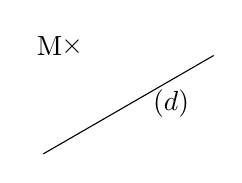
\begin{tikzpicture}[scale=0.5,every node/.style={scale=1},rotate=30]

\draw (0,2) node [left]{M};
\draw (0,2) node {$\times$};
\draw (-2,0)--(3,0) node [near end,below] {$(d)$};


\end{tikzpicture} 
 &  %manuel 6e, chapitre G3
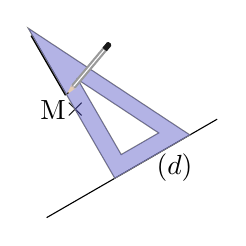
\begin{tikzpicture}[scale=0.5,every node/.style={scale=1},rotate=30]

\draw (0,2) node [left]{M};
\draw (0,2) node {$\times$};
\draw (-2,0)--(3,0) node [near end,below] {$(d)$};
\draw [thick](-0.02,4.2)--(-0.02,2.45);

%%%%%%%%%%%%%%%%%%%%%%%%
%%%%%%%%%%%%%%%%%%%%%%%%
%Définition des paramètres de l'équerre
%et de son positionnement
%%%%%%%%%%%%%%%%%%%%%%%%
%%%%%%%%%%%%%%%%%%%%%%%%

\def \xorigine {0}; %abscisse de l'origine de l'équerre posée avec un xshift
\def \yorigine {0}; %ordonnée de l'origine de l'équerre posée avec un yshift
\def \rotation {0}; %angle de rotation de l'équerre
\def \longueur {4}; %longueur de l'équerre
\def \largeur {2}; %largeur de l'équerre
\def \epaisseur {\longueur * 0.1}; %épaisseur de la partie «colorée» de l'équerre

%%%%%%%%%%%%%%%%%%%%%%%%
%%%%%%%%%%%%%%%%%%%%%%%%
%Tracé de l'équerre
%%%%%%%%%%%%%%%%%%%%%%%%
%%%%%%%%%%%%%%%%%%%%%%%%

\begin{scope}[scale=1.1,xshift=\xorigine cm,yshift=\yorigine cm,rotate=\rotation]

%contour extérieur de l'équerre
\coordinate (A) at (0,0) ; %«origine» de l'équerre
\coordinate (B) at (\largeur,0) ;
\coordinate (C) at (0,\longueur) ;
\draw [gray](A)--(B)--(C)--cycle;


%contour intérieur de l'équerre
\coordinate (D) at (\epaisseur,\epaisseur) ;
\coordinate (E) at ($\largeur*(1,0)-{\largeur * \epaisseur / \longueur}*(1,0)-\epaisseur*(1,0)+\epaisseur*(0,1)$);
\coordinate (F) at ($\epaisseur*(1,0)+\longueur*(0,1)-{2*\longueur * \epaisseur / \largeur}*(0,1)$);
\draw [gray](D)--(E)--(F)--cycle;

%partie colorée de l'équerre
\fill [color=blue!50!gray,opacity=.4,even odd rule] (A)--(B)--(C)--cycle (D)--(E)--(F)--cycle;%l'option even odd rule permet de faire le remplissage entre les 2 zones définies
\end{scope}

%%%%%%%%%%%%%%%%%%%%%%%%
%%%%%%%%%%%%%%%%%%%%%%%%
%Fin de l'équerre
%%%%%%%%%%%%%%%%%%%%%%%%
%%%%%%%%%%%%%%%%%%%%%%%%


%%%%%%%%%%%%%%%%%%%%%%%%
%%%%%%%%%%%%%%%%%%%%%%%%
%Début crayon
%%%%%%%%%%%%%%%%%%%%%%%%
%%%%%%%%%%%%%%%%%%%%%%%%

\begin{scope}[scale=0.35,xshift=0cm,yshift=7cm,rotate=-70] %le crayon, xshift et yshift pour les coordonnées de la pointe, rotate pour l'orientation du crayon
\def \couleur {black}
\coordinate (O) at (0,0);
\fill[\couleur!40] (-0.2,4.8) -- (0.2,4.8) -- (0.2,0.8) --(0.1,0.65) -- (0,0.8) -- (-0.1,0.66) -- (-0.2,0.8) -- cycle; %corps du crayon
\draw[color=white] (0,4.8) -- (0,0.8); %trait intérieur du crayon
\fill[\couleur!90] (-0.2,4.3) -- (0,4.27) -- (0.2,4.3) -- (0.2,4.8) arc(30:150:0.23cm); %partie haute du crayon
\fill[brown!40] (-0.2,0.8) -- (O)node[coordinate,pos=0.75](a){} -- (0.2,0.8)node[coordinate,pos=0.25](b){} -- (0.1,0.65) -- (0,0.8) -- (-0.1,0.66) -- cycle; %pointe du crayon (partie taillée)
\fill[\couleur!90] (a) -- (O) -- (b) -- cycle; %mine du crayon
\end{scope}

%%%%%%%%%%%%%%%%%%%%%%%%
%%%%%%%%%%%%%%%%%%%%%%%%
%Fin crayon
%%%%%%%%%%%%%%%%%%%%%%%%
%%%%%%%%%%%%%%%%%%%%%%%%


\end{tikzpicture} 
 & %manuel 6e, chapitre G3
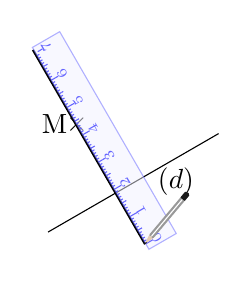
\begin{tikzpicture}[scale=0.5,every node/.style={scale=1},rotate=30]

\draw (0,2) node [left]{M};
\draw (0,2) node {$\times$};
\draw (-2,0)--(3,0) node [near end,below] {$(d)$};
\draw [thick](-0.02,4.2)--(-0.02,-1.5);

%%%%%%%%%%%%%%%%%%%%%%%%
%%%%%%%%%%%%%%%%%%%%%%%%
%Début règle
%%%%%%%%%%%%%%%%%%%%%%%%
%%%%%%%%%%%%%%%%%%%%%%%% 

    %Graduaton max. de la règle
    \def \Taille {7}
    %Définition de l 'angle de rotation de la règle
    \def \Rotation {90}
    %Définition du décalage de la règle
    \def \DecalX {0.4}
    \def \DecalY {-1.5}
    %Couleur des élèments de la règle (sauf le remplissage)
    \def \RegleColor {blue!60}

\begin{scope}[shift={(\DecalX,\DecalY)},rotate=\Rotation,scale=0.8]
    % contours de la règle
    \draw[color=\RegleColor, fill =blue!5, opacity=0.5] (-0.2,0.5) rectangle (\Taille+0.2,-0.5);	%Dont couleur de remplissage
    % graduation 1 mm
    \foreach \a in {0,0.1,...,\Taille}{\draw[color=\RegleColor] (\a,0.5)--(\a,0.42);}
    % graduation 5 mm
    \foreach \a in {0,0.5,...,\Taille}{\draw[color=\RegleColor] (\a,0.42)--(\a,0.35);}
    % graduation et repères 10 mm
    \foreach \a in {0,1,...,\Taille}{\draw[color=\RegleColor] (\a,0.35)--(\a,0.25)
    node[font=\tiny, rotate=\Rotation+30] (\a) at (\a,0.1){\a};}
\end{scope}

%%%%%%%%%%%%%%%%%%%%%%%%
%%%%%%%%%%%%%%%%%%%%%%%%
%Fin de la règle
%%%%%%%%%%%%%%%%%%%%%%%%
%%%%%%%%%%%%%%%%%%%%%%%%

%%%%%%%%%%%%%%%%%%%%%%%%
%%%%%%%%%%%%%%%%%%%%%%%%
%Début crayon
%%%%%%%%%%%%%%%%%%%%%%%%
%%%%%%%%%%%%%%%%%%%%%%%%

\begin{scope}[scale=0.35,xshift=-0.1cm,yshift=-4.28cm,rotate=-70] %le crayon, xshift et yshift pour les coordonnées de la pointe, rotate pour l'orientation du crayon
\def \couleur {black}
\coordinate (O) at (0,0);
\fill[\couleur!40] (-0.2,4.8) -- (0.2,4.8) -- (0.2,0.8) --(0.1,0.65) -- (0,0.8) -- (-0.1,0.66) -- (-0.2,0.8) -- cycle; %corps du crayon
\draw[color=white] (0,4.8) -- (0,0.8); %trait intérieur du crayon
\fill[\couleur!90] (-0.2,4.3) -- (0,4.27) -- (0.2,4.3) -- (0.2,4.8) arc(30:150:0.23cm); %partie haute du crayon
\fill[brown!40] (-0.2,0.8) -- (O)node[coordinate,pos=0.75](a){} -- (0.2,0.8)node[coordinate,pos=0.25](b){} -- (0.1,0.65) -- (0,0.8) -- (-0.1,0.66) -- cycle; %pointe du crayon (partie taillée)
\fill[\couleur!90] (a) -- (O) -- (b) -- cycle; %mine du crayon
\end{scope}

%%%%%%%%%%%%%%%%%%%%%%%%
%%%%%%%%%%%%%%%%%%%%%%%%
%Fin crayon
%%%%%%%%%%%%%%%%%%%%%%%%
%%%%%%%%%%%%%%%%%%%%%%%%


\end{tikzpicture} 
  &  %manuel 6e, chapitre G3
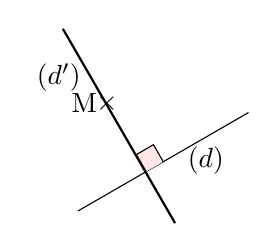
\begin{tikzpicture}[scale=0.5,every node/.style={scale=1},rotate=30]

\draw (0,2) node [left]{M};
\draw (0,2) node {$\times$};
\draw (-2,0)--(3,0) node [near end,below] {$(d)$};
\draw [thick](-0.02,4.2)--(-0.02,-1.5) node[near start,left]{$(d')$};
\draw [fill=pink!40!white](0,0)--(0,0.5)--(0.5,0.5)--(0.5,0);

\end{tikzpicture} 
 \\ 
 On trace une droite $d$ et on place un point $M$. & On place l'un des côtés de l'angle droit de l'équerre sur la droite $d$ et l'autre côté sur $M$.
 & On prolonge la droite à la règle. & On nomme la droite $d'$ et on code l'angle droit par un carré.\\

\end{tabularx} \\
 
 \end{exemple*1}


\exercice

En utilisant cette méthode, tracer un rectangle ABCD de longueur 3 cm et de longueur 5 cm.

%\correction

 
\end{methode*1}

\newpage

%%%%%%%%%%%%%%%%%%%%%%%%%%%%%

\begin{methode*1}[Construire la parallèle à une droite passant par un point]

\begin{exemple*1}
Trace une droite $d$ et place un point $M$ n'appartenant pas à la droite $d$.

Trace la droite $d'$ parallèle à la droite $d$ passant par le point $M$. \\[0.75em]

\begin{tabularx}{1.15\textwidth}{X|X|X|X}
\input{./PointsSegmentsDroites/figures/TracerParal_1}  &  %manuel 6e, chapitre G3
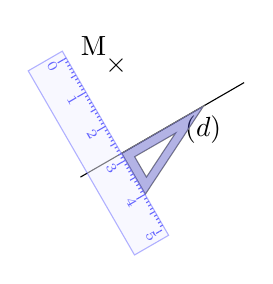
\begin{tikzpicture}[scale=.5,every node/.style={scale=1},rotate=30]

\draw (0,2) node [above left]{M};
\draw (0,2) node {$\times$};
\draw (-2.2,0)--(2.6,0) node [near end,below] {$(d)$};


%%%%%%%%%%%%%%%%%%%%%%%%
%%%%%%%%%%%%%%%%%%%%%%%%
%Définition des paramètres de l'équerre
%et de son positionnement
%%%%%%%%%%%%%%%%%%%%%%%%
%%%%%%%%%%%%%%%%%%%%%%%%

\def \xorigine {-1.65}; %abscisse de l'origine de l'équerre posée avec un xshift
\def \yorigine {0}; %ordonnée de l'origine de l'équerre posée avec un yshift
\def \rotation {-90}; %angle de rotation de l'équerre
\def \longueur {4}; %longueur de l'équerre
\def \largeur {2}; %largeur de l'équerre
\def \epaisseur {\longueur * 0.1}; %épaisseur de la partie «colorée» de l'équerre

%%%%%%%%%%%%%%%%%%%%%%%%
%%%%%%%%%%%%%%%%%%%%%%%%
%Tracé de l'équerre
%%%%%%%%%%%%%%%%%%%%%%%%
%%%%%%%%%%%%%%%%%%%%%%%%

\begin{scope}[scale=.6,xshift=\xorigine cm,yshift=\yorigine cm,rotate=\rotation]

%contour extérieur de l'équerre
\coordinate (A) at (0,0) ; %«origine» de l'équerre
\coordinate (B) at (\largeur,0) ;
\coordinate (C) at (0,\longueur) ;
\draw [gray](A)--(B)--(C)--cycle;


%contour intérieur de l'équerre
\coordinate (D) at (\epaisseur,\epaisseur) ;
\coordinate (E) at ($\largeur*(1,0)-{\largeur * \epaisseur / \longueur}*(1,0)-\epaisseur*(1,0)+\epaisseur*(0,1)$);
\coordinate (F) at ($\epaisseur*(1,0)+\longueur*(0,1)-{2*\longueur * \epaisseur / \largeur}*(0,1)$);
\draw [gray](D)--(E)--(F)--cycle;

%partie colorée de l'équerre
\fill [color=blue!50!gray,opacity=.4,even odd rule] (A)--(B)--(C)--cycle (D)--(E)--(F)--cycle;%l'option even odd rule permet de faire le remplissage entre les 2 zones définies

\end{scope}
%%%%%%%%%%%%%%%%%%%%%%%%
%%%%%%%%%%%%%%%%%%%%%%%%
%Fin de l'équerre
%%%%%%%%%%%%%%%%%%%%%%%%
%%%%%%%%%%%%%%%%%%%%%%%%

%%%%%%%%%%%%%%%%%%%%%%%%
%%%%%%%%%%%%%%%%%%%%%%%%
%Début règle !! Si la figure est tournée, il faut
%rajouter l'angle de rotation dans le node des graduation
%pour que les nombres soient écrits correctement
%%%%%%%%%%%%%%%%%%%%%%%%
%%%%%%%%%%%%%%%%%%%%%%%% 

    %Graduaton max. de la règle
    \def \Taille {5}
    %Définition de l 'angle de rotation de la règle
    \def \Rotation {-90}
    %Définition du décalage de la règle
    \def \DecalX {-1.5}
    \def \DecalY {2.8}
    %Couleur des élèments de la règle (sauf le remplissage)
    \def \RegleColor {blue!60}

\begin{scope}[shift={(\DecalX,\DecalY)},rotate=\Rotation,scale=1]
    % contours de la règle
    \draw[color=\RegleColor, fill =blue!5, opacity=0.5] (-0.2,0.5) rectangle (\Taille+0.2,-0.5);	%Dont couleur de remplissage
    % graduation 1 mm
    \foreach \a in {0,0.1,...,\Taille}{\draw[color=\RegleColor] (\a,0.5)--(\a,0.42);}
    % graduation 5 mm
    \foreach \a in {0,0.5,...,\Taille}{\draw[color=\RegleColor] (\a,0.42)--(\a,0.35);}
    % graduation et repères 10 mm
    \foreach \a in {0,1,...,\Taille}{\draw[color=\RegleColor] (\a,0.35)--(\a,0.25)
    node[font=\tiny, rotate=\Rotation+30] (\a) at (\a,0.1){\a};}%ici rajouter l'angle de rotation de la figure complète pour que les nombres soient écrits correctement
\end{scope}

%%%%%%%%%%%%%%%%%%%%%%%%
%%%%%%%%%%%%%%%%%%%%%%%%
%Fin de la règle
%%%%%%%%%%%%%%%%%%%%%%%%
%%%%%%%%%%%%%%%%%%%%%%%%


\end{tikzpicture} 
 & \input{./PointsSegmentsDroites/figures/TracerParal_3} &  %manuel 6e, chapitre G3
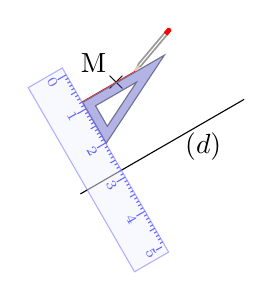
\begin{tikzpicture}[scale=.5,every node/.style={scale=1},rotate=30]

\draw (0,2) node [above left]{M};
\draw (0,2) node {$\times$};
\draw (-2.2,0)--(2.6,0) node [near end,below] {$(d)$};
\draw [red](-1,2)--(0.5,2);

%%%%%%%%%%%%%%%%%%%%%%%%
%%%%%%%%%%%%%%%%%%%%%%%%
%Définition des paramètres de l'équerre
%et de son positionnement
%%%%%%%%%%%%%%%%%%%%%%%%
%%%%%%%%%%%%%%%%%%%%%%%%

\def \xorigine {-1.65}; %abscisse de l'origine de l'équerre posée avec un xshift
\def \yorigine {0}; %ordonnée de l'origine de l'équerre posée avec un yshift
\def \rotation {-90}; %angle de rotation de l'équerre
\def \longueur {4}; %longueur de l'équerre
\def \largeur {2}; %largeur de l'équerre
\def \epaisseur {\longueur * 0.1}; %épaisseur de la partie «colorée» de l'équerre
\def \yorigine2 {3.31}; %ordonnée de l'origine de l'équerre posée avec un yshift

%%%%%%%%%%%%%%%%%%%%%%%%
%%%%%%%%%%%%%%%%%%%%%%%%
%Tracé de l'équerre
%%%%%%%%%%%%%%%%%%%%%%%%
%%%%%%%%%%%%%%%%%%%%%%%%

\begin{scope}[scale=.6,xshift=\xorigine cm,yshift=\yorigine2 cm,rotate=\rotation]

%contour extérieur de l'équerre
\coordinate (A) at (0,0) ; %«origine» de l'équerre
\coordinate (B) at (\largeur,0) ;
\coordinate (C) at (0,\longueur) ;
\draw [gray](A)--(B)--(C)--cycle;


%contour intérieur de l'équerre
\coordinate (D) at (\epaisseur,\epaisseur) ;
\coordinate (E) at ($\largeur*(1,0)-{\largeur * \epaisseur / \longueur}*(1,0)-\epaisseur*(1,0)+\epaisseur*(0,1)$);
\coordinate (F) at ($\epaisseur*(1,0)+\longueur*(0,1)-{2*\longueur * \epaisseur / \largeur}*(0,1)$);
\draw [gray](D)--(E)--(F)--cycle;

%partie colorée de l'équerre
\fill [color=blue!50!gray,opacity=.4,even odd rule] (A)--(B)--(C)--cycle (D)--(E)--(F)--cycle;%l'option even odd rule permet de faire le remplissage entre les 2 zones définies

\end{scope}
%%%%%%%%%%%%%%%%%%%%%%%%
%%%%%%%%%%%%%%%%%%%%%%%%
%Fin de l'équerre
%%%%%%%%%%%%%%%%%%%%%%%%
%%%%%%%%%%%%%%%%%%%%%%%%



%%%%%%%%%%%%%%%%%%%%%%%%
%%%%%%%%%%%%%%%%%%%%%%%%
%Début règle !! Si la figure est tournée, il faut
%rajouter l'angle de rotation dans le node des graduation
%pour que les nombres soient écrits correctement
%%%%%%%%%%%%%%%%%%%%%%%%
%%%%%%%%%%%%%%%%%%%%%%%% 

    %Graduaton max. de la règle
    \def \Taille {5}
    %Définition de l 'angle de rotation de la règle
    \def \Rotation {-90}
    %Définition du décalage de la règle
    \def \DecalX {-1.5}
    \def \DecalY {2.8}
    %Couleur des élèments de la règle (sauf le remplissage)
    \def \RegleColor {blue!60}

\begin{scope}[shift={(\DecalX,\DecalY)},rotate=\Rotation,scale=1]
    % contours de la règle
    \draw[color=\RegleColor, fill =blue!5, opacity=0.5] (-0.2,0.5) rectangle (\Taille+0.2,-0.5);	%Dont couleur de remplissage
    % graduation 1 mm
    \foreach \a in {0,0.1,...,\Taille}{\draw[color=\RegleColor] (\a,0.5)--(\a,0.42);}
    % graduation 5 mm
    \foreach \a in {0,0.5,...,\Taille}{\draw[color=\RegleColor] (\a,0.42)--(\a,0.35);}
    % graduation et repères 10 mm
    \foreach \a in {0,1,...,\Taille}{\draw[color=\RegleColor] (\a,0.35)--(\a,0.25)
    node[font=\tiny, rotate=\Rotation+30] (\a) at (\a,0.1){\a};}%ici rajouter l'angle de rotation de la figure complète pour que les nombres soient écrits correctement
\end{scope}

%%%%%%%%%%%%%%%%%%%%%%%%
%%%%%%%%%%%%%%%%%%%%%%%%
%Fin de la règle
%%%%%%%%%%%%%%%%%%%%%%%%
%%%%%%%%%%%%%%%%%%%%%%%%

%%%%%%%%%%%%%%%%%%%%%%%%
%%%%%%%%%%%%%%%%%%%%%%%%
%Début crayon
%%%%%%%%%%%%%%%%%%%%%%%%
%%%%%%%%%%%%%%%%%%%%%%%%

\begin{scope}[scale=0.3,xshift=1.65cm,yshift=6.65cm,rotate=-70] %le crayon, xshift et yshift pour les coordonnées de la pointe, rotate pour l'orientation du crayon
\def \couleur {black}
\coordinate (O) at (0,0);
\fill[\couleur!40] (-0.2,4.8) -- (0.2,4.8) -- (0.2,0.8) --(0.1,0.65) -- (0,0.8) -- (-0.1,0.66) -- (-0.2,0.8) -- cycle; %corps du crayon
\draw[color=white] (0,4.8) -- (0,0.8); %trait intérieur du crayon
\fill[red] (-0.2,4.3) -- (0,4.27) -- (0.2,4.3) -- (0.2,4.8) arc(30:150:0.23cm); %partie haute du crayon
\fill[brown!40] (-0.2,0.8) -- (O)node[coordinate,pos=0.75](a){} -- (0.2,0.8)node[coordinate,pos=0.25](b){} -- (0.1,0.65) -- (0,0.8) -- (-0.1,0.66) -- cycle; %pointe du crayon (partie taillée)
\fill[red] (a) -- (O) -- (b) -- cycle; %mine du crayon
\end{scope}

%%%%%%%%%%%%%%%%%%%%%%%%
%%%%%%%%%%%%%%%%%%%%%%%%
%Fin crayon
%%%%%%%%%%%%%%%%%%%%%%%%
%%%%%%%%%%%%%%%%%%%%%%%%


\end{tikzpicture} 
\\ 
On trace une droite $d$, on place un point $M$. On place l'un des côtés de l'angle droit de l'équerre sur la droite $d$. & On place la règle le long de l'autre côté de l'équerre & On tient bien la règle et on fait coulisser l'équerre le long de la règle, jusqu'au point $M$. & On trace ainsi la droite $d'$ et on obtient :\vspace{0.3em}
%manuel 6e, chapitre G3
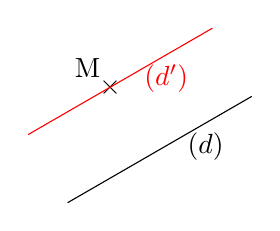
\begin{tikzpicture}[scale=.5,every node/.style={scale=1},rotate=30]

\draw (0,2) node [above left]{M};
\draw (0,2) node {$\times$};
\draw (-2.4,0)--(3,0) node [near end,below] {$(d)$};
\draw [red](-2.4,2)--(3,2) node [near end,below] {$(d')$};

\end{tikzpicture} 
\\
\end{tabularx} \\
 \end{exemple*1}

\exercice

Trace dans ton cahier un segment $[AB]$ d'une longueur de 5 cm et place un point $C$ au-dessus du segment $[AB]$ ($C$ n'est pas sur le segment). Construis, en rouge, la perpendiculaire à $[AB]$ passant par $C$. Construis, en vert, la parallèle à $[AB]$ passant par $C$.
%\correction

\end{methode*1}

\begin{aconnaitre}
\textbf{\underline{Propriété:}}\\
Si deux droites sont parallèles et si une troisième droite est perpendiculaire à l'une d'elle, alors elles est perpendiculaire à l'autre.
\end{aconnaitre}

\begin{methode*1}[Illustration]
\begin{exemple*1}

Soit $(d)$ et $(d')$ deux droites parallèles. Soit $(\Delta)$ un troisième droite.\\
Si $(d)$ et $(\Delta)$ sont perpendiculaires alors $(d')$ et $(\Delta)$ sont également perpendicualires.

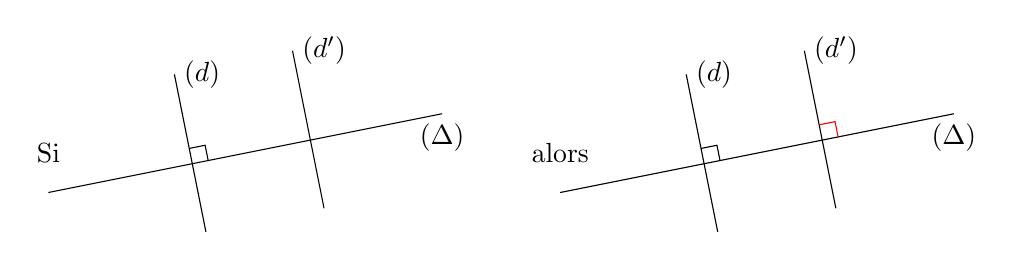
\begin{tikzpicture}
\draw (-2.0,0) node {Si} (-2,-0.5) -- ++(5,1) node[below] {$(\Delta)$} ;
%\draw (-2.0,0) node {Si} (-2,-0.5) ++(1,0.2) -- ++(4,0.8) node[below] {$(\Delta)$} ;
\draw (0,-1) -- ++(-0.4,2) node[right] {$(d)$};
\draw (1.5,-0.7) -- ++(-0.4,2) node[right] {$(d^\prime)$};
\draw (-0.17,-0.14) ++(0.2,0.04) -- ++(-0.04,0.2) -- ++(-0.2, -0.04); %circle (1pt);


\draw (4.5,0) node {alors} ++(0,-0.5) -- ++(5,1) node[below] {$(\Delta)$} ;
\draw (6.5,-1) -- ++(-0.4,2) node[right] {$(d)$};
\draw (8.0,-0.7) -- ++(-0.4,2) node[right] {$(d^\prime)$};
\draw (6.33,-0.14) ++(0.2,0.04) -- ++(-0.04,0.2) -- ++(-0.2, -0.04);
\draw[red] (7.83,0.16) ++(0.2,0.04) -- ++(-0.04,0.2) -- ++(-0.2, -0.04); %circle (1pt);

\end{tikzpicture}
\end{exemple*1}

\exercice

Dans la figure ci-contre:\
\begin{itemize}
\item Tracer la droite $(AB)$.
\item Construire la droite $(d)$ parallèle à $(AB)$ passant par $C$.
\item Construire la droite $(d')$ perpendiculaire à $(AB)$ passant par $B$.
\item Que peut-on dire des droites $(d)$ et $(d')$? Justifier.\\
\end{itemize}
\begin{center}
\tikzset{
   cross/.pic = {
     \draw[thick] (-0.2,0.2) -- (0.2,-0.2);
     \draw[thick] (-0.2,-0.2) -- (0.2,0.2);}
}


\begin{tikzpicture}
\draw (0,0) rectangle (10,6);
\pic[scale=0.6] at (1,3) {cross}; \draw (1,3.5) node {\large $A$};
\pic[scale=0.6] at (6,5) {cross}; \draw (6,5.5) node {\large $B$};
\pic[scale=0.6] at (9,2) {cross}; \draw (9,2.5) node {\large $C$};
\end{tikzpicture}
\end{center}
\end{methode*1}


%%%%%%%%%%%%%%%%%%%%%%%%%%%%%
\newpage

\section{La médiatrice}

\begin{definition}
La \textbf{\MotDefinition{médiatrice}{}} d'un segment est la droite qui coupe ce segment perpendiculairement en son milieu.
\end{definition}


\begin{methode*1}[Construire une médiatrice]

\begin{exemple*1}
Trace un segment $[OS]$ de longueur 5 cm puis sa médiatrice. \\[0.75em]

\begin{tabularx}{\textwidth}{X|X|X|X}
%manuel 6e, chapitre G3

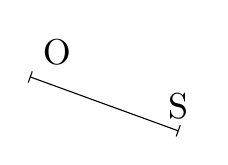
\begin{tikzpicture}[scale=0.5,every node/.style={scale=1.3}]

\def \CharSize {2.5};

\begin{scope}[rotate=-20]
\draw (-2,0)--(2,0);
\draw (-2,0)--+(90:0.15)--+(-90:0.15);
\draw (2,0)--+(90:0.15)--+(-90:0.15);
\node [above right] at (-2,0) {O};
\node [above] at (2,0) {S};
\end{scope}

\end{tikzpicture}  &

% Attention, il faut déclarer la librairie calc :\usetikzlibrary{calc}  pour les calculs de coordonnées des points


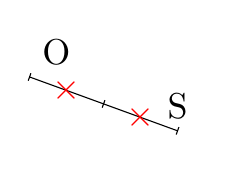
\begin{tikzpicture}	[scale=0.5,every node/.style={scale=1.3}]

\begin{scope}[rotate=-20] %la figure
\draw (-2,0)--(0,0) node [midway,red] {$\times$};
\draw (0,0)--(2,0) node [midway,red] {$\times$};
\draw (-2,0)--+(90:0.1)--+(-90:0.1);
\draw (2,0)--+(90:0.1)--+(-90:0.1);
\draw (0,0)--+(90:0.1)--+(-90:0.1);
\node [above right] at (-2,0) {O};
\node [above] at (2,0) {S};
\end{scope}

\end{tikzpicture} 
 
 & 
% Attention, il faut déclarer la librairie calc :\usetikzlibrary{calc}  pour les calculs de coordonnées des points

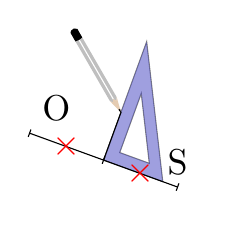
\begin{tikzpicture}[scale=0.5,every node/.style={scale=1.3}]
  
%%%%%%%%%%%%%%%%%%%%%%%%
%%%%%%%%%%%%%%%%%%%%%%%%
%Définition des paramètres de l'équerre
%et de son positionnement
%%%%%%%%%%%%%%%%%%%%%%%%
%%%%%%%%%%%%%%%%%%%%%%%%

\def \xorigine {0}; %abscisse de l'origine de l'équerre posée avec un xshift
\def \yorigine {0}; %ordonnée de l'origine de l'équerre posée avec un yshift
\def \rotation {-20}; %angle de rotation de l'équerre
\def \longueur {4}; %longueur de l'équerre
\def \largeur {2}; %largeur de l'équerre
\def \epaisseur {\longueur * 0.1}; %épaisseur de la partie «colorée» de l'équerre

%%%%%%%%%%%%%%%%%%%%%%%%
%%%%%%%%%%%%%%%%%%%%%%%%
%Tracé de l'équerre
%%%%%%%%%%%%%%%%%%%%%%%%
%%%%%%%%%%%%%%%%%%%%%%%%
\begin{scope}[scale=0.8,xshift=\xorigine cm,yshift=\yorigine cm,rotate=\rotation]

%contour extérieur de l'équerre
\coordinate (A) at (0,0) ; %«origine» de l'équerre
\coordinate (B) at (\largeur,0) ;
\coordinate (C) at (0,\longueur) ;
\draw [gray](A)--(B)--(C)--cycle;


%contour intérieur de l'équerre
\coordinate (D) at (\epaisseur,\epaisseur) ;
\coordinate (E) at ($\largeur*(1,0)-{\largeur * \epaisseur / \longueur}*(1,0)-\epaisseur*(1,0)+\epaisseur*(0,1)$);
\coordinate (F) at ($\epaisseur*(1,0)+\longueur*(0,1)-{2*\longueur * \epaisseur / \largeur}*(0,1)$);
\draw [gray](D)--(E)--(F)--cycle;

%partie colorée de l'équerre
\fill [color=blue!50!gray,opacity=0.5,even odd rule] (A)--(B)--(C)--cycle (D)--(E)--(F)--cycle;%l'option even odd rule permet de faire le remplissage entre les 2 zones définies

\end{scope}

\begin{scope}[scale=0.5,xshift=.32cm,yshift=3cm,rotate=30] %le crayon
\fill[gray!50] (0,4) -- (0.4,4) -- (0.4,0) --(0.3,-0.15) -- (0.2,0) -- (0.1,-0.14) -- (0,0) -- cycle;
\draw[color=white] (0.2,4) -- (0.2,0);
\fill[black] (0,3.5) -- (0.2,3.47) -- (0.4,3.5) -- (0.4,4) arc(30:150:0.23cm);
\fill[brown!40] (0,0) -- (0.2,-0.8)node[coordinate,pos=0.75](a){} --(0.4,0) node[coordinate,pos=0.25](b){} -- (0.3,-0.15) -- (0.2,0) -- (0.1,-0.14) -- cycle;
\fill[black] (a) -- (0.2,-0.8) -- (b) -- cycle;
\end{scope}

\begin{scope}[rotate=-20] %la figure
\draw (-2,0)--(0,0) node [midway,red] {$\times$};
\draw (0,0)--(2,0) node [midway,red] {$\times$};
\draw (-2,0)--+(90:0.1)--+(-90:0.1);
\draw (2,0)--+(90:0.1)--+(-90:0.1);
\draw (0,0)--+(90:0.1)--+(-90:0.1);
\node [above right] at (-2,0) {O};
\node [above] at (2,0) {S};

\draw (0,0)--($(0,0)!1.3cm!90:(2,0)$); %trace un segment de 1.3cm à 90° du segment allant de (0,0) à (2,0)

\end{scope}



\end{tikzpicture} 
  &  \input{./PointsSegmentsDroites/figures/Mediatrice4}  \\ 
On trace un segment $[OS]$. & On trace le milieu du segment. & On trace la droite perpendiculaire au segment qui passe par ce milieu. & On code l'angle droit par un carré. \\
\end{tabularx} \\

 \end{exemple*1}
 
 \begin{exemple*1}
Trace un segment $[AB]$ de longueur 6 cm. Construis sa médiatrice au compas. \\[0.75em]

\begin{tabular}{l|l|l|l}
 \textcolor{H1}{\circled{1}} &  \textcolor{H1}{\circled{2}} &  \textcolor{H1}{\circled{3}} & \textcolor{H1}{\circled{1}} On trace le segment $[AB]$. \\ 
 \multirow{7}{*}{

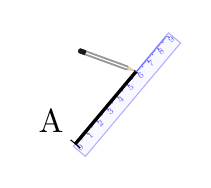
\begin{tikzpicture}[scale=0.2,rotate=50,every node/.style={scale=1.2}]

%début de la règle
    %Graduaton max. de la règle
    \def \Taille {9}
    %Définition de l 'angle de rotation de la règle
    \def \Rotation {0}
    %Définition du décalage de la règle
    \def \DecalX {0}
    \def \DecalY {0}
    %Couleur des élèments de la règle (sauf le remplissage)
    \def \RegleColor {blue!60}

\begin{scope}[scale=1,shift={(\DecalX,\DecalY)},rotate=\Rotation]
    % contours de la règle
    \draw[color=\RegleColor, fill =blue!5, opacity=0.5] (-0.2,0.5) rectangle (\Taille+0.2,-0.5);	%Dont couleur de remplissage
    % graduation 1 mm
    \foreach \a in {0,0.1,...,\Taille}{\draw[color=\RegleColor] (\a,0.5)--(\a,0.42);}
    % graduation 5 mm
    \foreach \a in {0,0.5,...,\Taille}{\draw[color=\RegleColor] (\a,0.42)--(\a,0.35);}
    % graduation et repères 10 mm
    \foreach \a in {0,1,...,\Taille}{\draw[color=\RegleColor] (\a,0.35)--(\a,0.25)
    node[scale=0.5,font=\tiny, rotate=40] (\a) at (\a,0.1){\a};}
%fin de la règle

\draw (0,0.5) node[above left]{A};
\draw (0,0.5)--+(90:0.4)--+(-90:0.4);
\draw [very thick](0,0.5)--(6,0.5);

\end{scope}

\begin{scope}[scale=0.8,xshift=7.52cm,yshift=.62cm,rotate=20] %le crayon, xshift et yshift pour les coordonnées de la pointe, rotate pour l'orientation du crayon
\def \couleur {black}
\coordinate (O) at (0,0);
\fill[\couleur!40] (-0.2,4.8) -- (0.2,4.8) -- (0.2,0.8) --(0.1,0.65) -- (0,0.8) -- (-0.1,0.66) -- (-0.2,0.8) -- cycle; %corps du crayon
\draw[color=white] (0,4.8) -- (0,0.8); %trait intérieur du crayon
\fill[\couleur!90] (-0.2,4.3) -- (0,4.27) -- (0.2,4.3) -- (0.2,4.8) arc(30:150:0.23cm); %partie haute du crayon
\fill[brown!40] (-0.2,0.8) -- (O)node[coordinate,pos=0.75](a){} -- (0.2,0.8)node[coordinate,pos=0.25](b){} -- (0.1,0.65) -- (0,0.8) -- (-0.1,0.66) -- cycle; %pointe du crayon (partie taillée)
\fill[\couleur!90] (a) -- (O) -- (b) -- cycle; %mine du crayon
\end{scope}


\end{tikzpicture}


} &  \multirow{7}{*}{

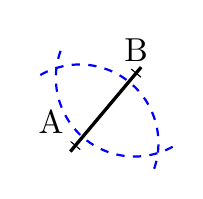
\begin{tikzpicture}[scale=0.2,rotate=50,every node/.style={scale=1.2}]

\draw [very thick](-0.5,0.5)--(6.5,0.5);
\draw (0,0.5)--+(90:0.4)--+(-90:0.4);
\draw (6,0.5)--+(90:0.4)--+(-90:0.4);
\draw (0,0.5) node[above left]{A};
\draw (6,0.5) node[above]{B};

\draw [style=dashed,color=blue,thick](4,5.083) arc (110:250:5);
\draw [style=dashed,color=blue,thick](2,5.083) arc (70:-70:5);
%\draw (3,6)--(3,-6);

\coordinate (A) at (0,0.5) ;
\coordinate (B) at (2,5.083) ;
\begin{scope}[scale=.8]
\Compas{A}{B}
\end{scope}

\end{tikzpicture}
} & \multirow{7}{*}{

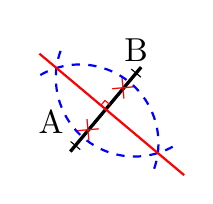
\begin{tikzpicture}[scale=0.2,rotate=50,every node/.style={scale=1.2}]

%\draw [very thick](-0.5,0.5)--(6.5,0.5);
\draw [very thick](-0.5,0.5)--(3,0.5) node[midway,red,rotate=50]{$\times$}--(6.5,0.5)node[midway,red,rotate=50]{$\times$};
\draw (0,0.5)--+(90:0.4)--+(-90:0.4);
\draw (6,0.5)--+(90:0.4)--+(-90:0.4);
\draw (0,0.5) node[above left]{A};
\draw (6,0.5) node[above]{B};

\draw [style=dashed,color=blue,thick](4,5.083) arc (110:250:5);
\draw [style=dashed,color=blue,thick](2,5.083) arc (70:-70:5);
\draw [thick,color=red](3,6)--(3,-6);
\draw [color=red](3,0.9)-|(3.4,0.5);

\end{tikzpicture}
} &  \textcolor{H1}{\circled{2}} On trace deux arcs de cercle\\ % exemple de fusion de cellules d'une même colonne
&&& de centres $A$ et $B$, de même\\ 
&&& rayon, en choisissant un\\
&&& rayon suffisamment grand\\
&&& pour que ces arcs se coupent\\
&&&  en deux points.\\ 
&&& \textcolor{H1}{\circled{3}} La médiatrice de [AB] est \\
&&&  la droite qui passe par ces\\
&&& deux points.\\ 
\end{tabular} \\

 \end{exemple*1}

\exercice 
Trace un segment $[AB]$ de 7 cm. Trace la médiatrice du segment $[AB]$ par la méthode de ton choix.
%\correction

 
\end{methode*1}

%%%%%%%%%%%%%%%%%%%%%%%%%%%%%


\section{Les angles}

%%%%%%%%%%%%%%%%%%%%%%%%%%%%%

% remarque : pour qu'un mot se retrouve dans le lexique : \MotDefinition{asymptote horizontale}{} 

\begin{definition}
Un \MotDefinition{angle}{} est une portion de plan délimitée par deux demi-droites ayant la même origine.
 \end{definition}

\subsection{Reconnaître les différents types d'angles}

On classe les angles par catégories selon leur mesure.

 \renewcommand*\tabularxcolumn[1]{>{\centering\arraybackslash}m{#1}}
 \begin{ttableau}{\linewidth}{6}
\hline \textbf{Angle} 	&	Nul	&	Aigu		&	Droit		&	Obtus	&	Plat	\\ \hline
 \textbf{Figure} 	&	\includegraphics[width=1.7cm]{angle_nul}	&	\includegraphics[width=1.7cm]{angle_aigu}	&	\includegraphics[width=1.7cm]{angle_droit}	&	\includegraphics[width=1.7cm]{angle_obtus}	&	\includegraphics[width=1.7cm]{angle_plat}	\\ \hline
 \textbf{Mesure} 	&	$0^\circ$	&	entre $0^\circ$ et $90^\circ$	&	$90^\circ$		&	entre $90^\circ$ et $180^\circ$	&	 $180^\circ$	\\ \hline
 \multirow{3}{*}{} \textbf{Position} 	&		&	&	&	&	dans le 	\\ 
 \textbf{des}	&	confondus		&	&	perpendiculaires	&	&	 prolongement	\\
\textbf{côtés}	&	&	&	&	&	 l'un de l'autre	\\ \hline
 \end{ttableau}

%%%%%%%%%%%%%%%%%%%%%%%%%%%%%

\begin{methode*1}[Nommer un angle]

\begin{exemple*1}
Nomme l'angle marqué en violet sur la figure ci‑dessous.  \\[0.75em]

\begin{minipage}[c]{0.70\textwidth}
Le sommet de l'angle est le point $C$ : c'est la lettre centrale. \\[0.5em]
Les côtés de l'angle sont les demi‑droites $[CH)$ (ou $[Cx)$) et $[CS)$ (ou $[CA)$ (ou $[Cy)$). \\[0.5em]
Cet angle peut se nommer : $\widehat{{\textcolor{A1}{H}}C{\textcolor{C1}{S}}}$; $\widehat{{\textcolor{C1}{S}}C{\textcolor{A1}{H}}}$ ; $\widehat{{\textcolor{A1}{H}}C{\textcolor{C1}{A}}}$ ; $\widehat{{\textcolor{C1}{A}}C{\textcolor{A1}{H}}}$ ; $\widehat{{\textcolor{C1}{y}}C{\textcolor{A1}{x}}}$.
 \end{minipage} \hfill%
 \begin{minipage}[c]{0.26\textwidth}
 \includegraphics[width=3.8cm]{nommer_angle}
 \end{minipage} \\
 
\end{exemple*1}

\exercice 
Nomme les angles marqués sur la figure ci‑dessous. 
\begin{center} \includegraphics[width=4.5cm]{nommer_angles} \end{center}
%\correction
 
\end{methode*1}

%%%%%%%%%%%%%%%%%%%%%%%%%%%%%

\begin{methode*1}[Utiliser le rapporteur]

\begin{exemple*1}
Mesure l'angle $\widehat{CAB}$. \\[0.75em]

\begin{minipage}[c]{0.49\textwidth}
\centering
\includegraphics[width=4.8cm]{rapporteur1}
\end{minipage}\hfill%
 \begin{minipage}[c]{0.49\textwidth}%
 \centering
 \includegraphics[width=6.6cm]{rapporteur2}
  \end{minipage} \\
 \begin{minipage}[c]{0.43\textwidth}
On place le centre du rapporteur sur le sommet de l'angle.
\end{minipage} \hfill%
 \begin{minipage}[c]{0.53\textwidth}
 On place un zéro du rapporteur sur le côté $[AC)$. Si besoin, on prolonge la demi‑droite $[AC)$. La mesure de l'angle est donnée par l'autre côté de l'angle sur \underline{la même échelle} de graduation.
 \end{minipage} \\
  \end{exemple*1}
 
 \begin{exemple*1}
Construis un angle $\widehat{BUT}$ de $108^\circ$.  \\[0.75em]

\begin{minipage}[c]{0.49\textwidth}
\centering
\includegraphics[width=4.8cm]{rapporteur3}
\end{minipage}\hfill%
 \begin{minipage}[c]{0.49\textwidth}%
 \centering
 \includegraphics[width=6.6cm]{rapporteur44}
  \end{minipage} \\
 \begin{minipage}[c]{0.43\textwidth}
On trace $[UB)$, premier côté de l'angle. On place le centre du rapporteur sur le point $U$.
\end{minipage} \hfill%
 \begin{minipage}[c]{0.53\textwidth}
 On place un zéro du rapporteur sur le côté $[UB)$. On marque, d'un petit trait-repère, $108^\circ$ avec la bonne graduation.
On trace la demi‑droite d'origine $U$ passant par le repère. On place un point $T$ sur cette demi‑droite.
  \end{minipage} \\
  \end{exemple*1}
 
\exercice
 \begin{enumerate}
 \begin{minipage}[c]{0.36\textwidth}
  \item Mesure l'angle $\widehat{xOy}$ ci‑contre ;
  \item Construis un angle $\widehat{SAT}$ de $85^\circ$. 
  \end{minipage} \hfill%
 \begin{minipage}[c]{0.56\textwidth}
  \includegraphics[width=6cm]{angleyOx} 
  \end{minipage} \\
  \end{enumerate}
%\correction
 
\end{methode*1}

%%%%%%%%%%%%%%%%%%%%%%%%%%%%%


\section{La bissectrice}

\begin{definition}
La \textbf{\MotDefinition{bissectrice}{}} d'un angle est la demi-droite qui a pour origine le sommet de l'angle et qui partage l'angle en deux angles de même mesure.
\end{definition}


\begin{methode*1}[Construire une bissectrice]


\begin{exemple*1} \\[0.75em]
Trace un angle $\widehat{xOy}$. Construis sa bissectrice au compas. \\[0.5em]

\begin{tabularx}{\textwidth}{X|X|X}
 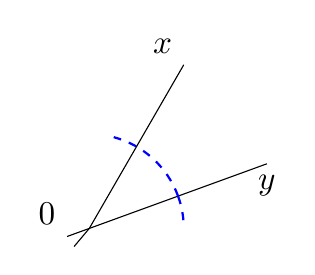
\begin{tikzpicture}[scale=0.6,rotate=20,every node/.style={scale=1.2}]

\draw (-0.5,0) node[above left]{0}--(4,0) node[below]{$y$};
\draw (0,0) --(40:4) node[above left]{$x$};
\draw (0,0)--+(210:0.5);
\draw[thick,dashed,blue] (2,0) arc (0:55:2);
\draw[thick,dashed,blue] (2,0) arc (0:-15:2);

\coordinate (A) at (0,0) ;
\coordinate (B) at (1.414,1.414) ;


\begin{scope}[scale=0.35]
\Compas{A}{B}
\end{scope}


\end{tikzpicture}

 &  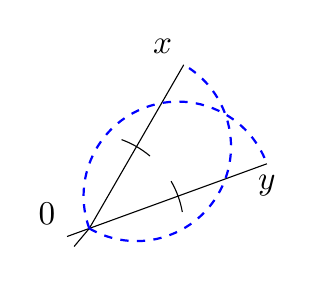
\begin{tikzpicture}[scale=0.6,rotate=20,every node/.style={scale=1.2}]

\draw (-0.5,0) node[above left]{0}--(4,0) node[below]{$y$};
\draw (0,0) --(40:4) node[above left]{$x$};
\draw (0,0)--+(210:0.5);

\draw (1.532,1.286) arc (40:50:2);
\draw (1.532,1.286) arc (40:30:2);
\draw (2,0) arc (0:10:2);
\draw (2,0) arc (0:-10:2);

\draw [thick,blue,dashed](0,0) arc (180:0:2);
\draw [thick,blue,dashed](0,0) arc (-140:40:2);

%\draw (2,0) node{$\bullet$};
%\draw (1.532,1.286) node{$\bullet$};
%\draw (0,0)--(4.698,1.71);

\coordinate (A) at (1.532,1.286) ;
\coordinate (B) at (3.064,2.572) ;

\begin{scope}[scale=0.35]
\Compas{A}{B}
\end{scope}


\end{tikzpicture}

 & 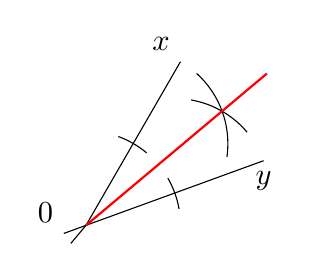
\begin{tikzpicture}[scale=0.6,rotate=20,every node/.style={scale=1.1}]

\draw (-0.5,0) node[above left]{0}--(4,0) node[below]{$y$};
\draw (0,0) --(40:4) node[above left]{$x$};
\draw (0,0)--+(210:0.5);

\draw (1.532,1.286) arc (40:50:2);
\draw (1.532,1.286) arc (40:30:2);
\draw (2,0) arc (0:10:2);
\draw (2,0) arc (0:-10:2);
\draw (3,1.732) arc (60:20:2);
\draw (3.3,2.221) arc (28:-28:2);

\draw [red,thick](0,0)--(4.698,1.71);


\end{tikzpicture}

 \\ 
Au compas, on trace un arc de cercle de centre $O$ qui coupe chaque côté de l'angle en un point. & On trace deux arcs de cercle de même rayon ayant ces deux points pour centres. Ces arcs se coupent en un point. & La bissectrice de l'angle $\widehat{xOy}$ est la demi-droite d'origine $O$ passant par ce point. \\
\end{tabularx} \\

 \end{exemple*1}

\exercice 

Trace un triangle $ABC$ tel que $AB=4$\,cm ; $AC=7$\,cm ; $BC=5$\,cm ; puis trace les bissectrices des angles $\widehat{ABC}$ ; $\widehat{BAC}$ et $\widehat{ACB}$. Que remarques-tu ?

%\correction

 
\end{methode*1}

%%%%%%%%%%%%%%%%%%%%%%%%%%%%%

%%%%%%%%Mise en page
\newpage
%%%%%%%%%%%%%%%%%%%%



\section{Le cercle}

\begin{definition}
Un \textbf{\MotDefinition{cercle}{}} de centre $O$ est l'ensemble des points situés à la même distance du point $O$. 
Cette distance est le \textbf{\MotDefinition{rayon}{}} du cercle.
\end{definition}

\begin{aconnaitre}
\begin{tabularx}{.95\linewidth}{|X|p{5cm}|p{3cm}|}
\hline
\multirow{5}{*}{\includegraphics[width=3.4cm]{cercleAFNME}}  & Le \textcolor{C2}{\textbf{centre}} d'un cercle est le point équidistant de tous les points qui constituent ce cercle. & Le point $O$ est le \textcolor{C2}{\textbf{centre}} du cercle $(\mathcal{C})$.\\ \cline{2-3}
 & Un \textcolor{J1}{\textbf{rayon}} d'un cercle est un segment ayant pour extrémités le centre et un point de ce cercle. & Le segment $[OA]$ est un  \textcolor{J1}{\textbf{rayon}} du cercle $(\mathcal{C})$.\\ \cline{2-3}
  & Un  \textcolor{H1}{\textbf{diamètre}} d'un cercle est un segment ayant pour extrémités deux points de ce cercle et contenant son centre. & Le segment $[EF]$ est un  \textcolor{H1}{\textbf{diamètre}} du cercle $(\mathcal{C})$.\\ \cline{2-3}
 & Une  \textcolor{PartieFonction}{\textbf{corde}} d'un cercle est un segment ayant pour extrémités deux points de ce cercle. & Le segment $[MN]$ est une  \textcolor{PartieFonction}{\textbf{corde}} du cercle $(\mathcal{C})$.\\ \cline{2-3}
 & Un  \textcolor{B2}{\textbf{arc de cercle}} est une portion de cercle comprise entre deux points de ce cercle. & La portion de cercle $\overset{\huge{\frown}}{MN}$ comprise entre $M$ et $N$ est un  \textcolor{B2}{\textbf{arc du cercle}} $(\mathcal{C})$.\\ \hline
  \end{tabularx}
 \end{aconnaitre}
  
  
 \begin{remarque}
 Par commodité de langage, on appelle « rayon » la longueur du rayon d'un cercle, et  on appelle « diamètre » la longueur de son diamètre.
  \end{remarque}
  
 \begin{remarque}
 Le diamètre d'un cercle est égal au double de son rayon.
  \end{remarque}

\exercicesbase
\begin{colonne*exercice}

\serie{codage}


\begin{exercice}[placer les points]
Place les points A, B, C, D et E sur la figure sachant que:
\begin{itemize}
    \item E est le milieu de [BC]
	\item $(AC)\bot (BC)$
    \item AD=BD
\end{itemize}
\begin{center}
    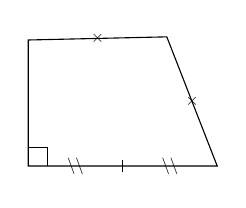
\begin{tikzpicture}[scale=0.8,every node/.style={scale=0.6}]

\draw (0,0)--(3,0)--(2.2,2.05)--(0,2)--cycle;
\draw (0.3,0)|-(0,0.3);
\draw (1.5,0.1)--(1.5,-0.1);
\draw (0.75,0) node {$\backslash \backslash$};
\draw (2.25,0) node {$\backslash \backslash$};
\draw (1.1,2.02) node {$\times$};
\draw (2.6,1.02) node {$\times$};

\end{tikzpicture}
\end{center}
\end{exercice}

\begin{exercice}[lire le codage]
Donne la liste des renseignements codés sur la figure.
\begin{center}
    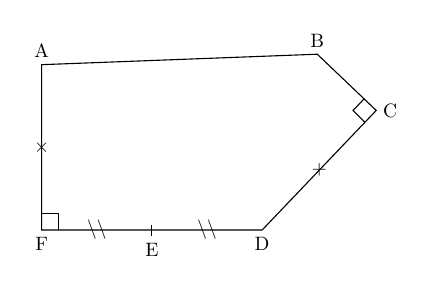
\begin{tikzpicture}[scale=0.7,every node/.style={scale=0.7}]

\draw (0,3) node[above] {A}--(5,3.19) node[above] {B}--(6.07,2.17) node[right]{C}--(4,0) node[below]{D}--(2,0)node[below=0.8mm]{E}--(0,0) node[below]{F}--cycle;
\draw (0.3,0)|-(0,0.3);
\draw (5.85,2.38) -- (5.65,2.17)--(5.86,1.96);
\draw (2,0.1)--(2,-0.1);
\draw (1,0) node {$\backslash \backslash$};
\draw (3,0) node {$\backslash \backslash$};
\draw (0,1.5) node {$\times$};
\draw (5.035,1.085) node[rotate=45] {$\times$};

\end{tikzpicture}

\end{center}
\end{exercice}

\begin{exercice}[coder]
Code les figures selon les indications données.
\begin{colenumerate}{2}
 \item
 
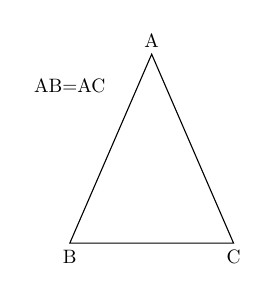
\begin{tikzpicture}[scale=0.8,every node/.style={scale=0.7}]

\draw (1.3,3) node[above] {A}--(0,0) node[below] {B}--(2.6,0) node[below]{C}--cycle;
\node at (0,2.5) {AB=AC};

\end{tikzpicture}
  \item
  
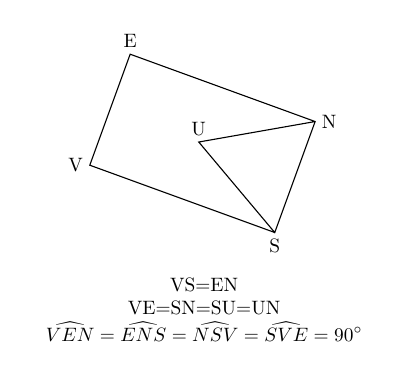
\begin{tikzpicture}[scale=0.5,every node/.style={scale=0.7},rotate=-20]

\draw (5,0) node[below]{S}--(0,0) node [left]{V}--(0,3) node[above] {E}--(5,3) node[right] {N}--(5,0) --(2.4,1.5) node[above]{U}--(5,3);
\node at(4,-2.5) {\begin{tabular}{c} VS=EN \\ VE=SN=SU=UN \\ $\widehat{VEN}=\widehat{ENS}=\widehat{NSV}=\widehat{SVE}=90^\circ$ \end{tabular}};

\end{tikzpicture}
  \item
  
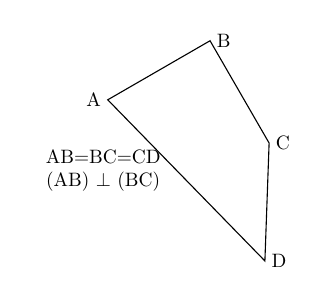
\begin{tikzpicture}[scale=0.5,every node/.style={scale=0.7},rotate=-60]

\draw (0,0) node [left]{A}--(0,3) node[right] {B}--(3,3) node[right] {C}--(5.54,1.41) node[right]{D}--cycle;
\node at(1.5,-1) {\begin{tabular}{c} AB=BC=CD \\ (AB) $\perp$ (BC) \end{tabular}};

\end{tikzpicture}
  \item

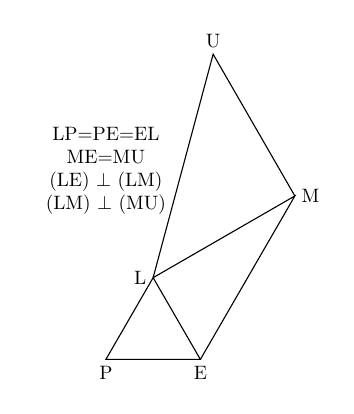
\begin{tikzpicture}[scale=0.6,every node/.style={scale=0.7},rotate=0]

\draw (0,0) node [below]{P}--(2,0) node[below] {E}--(1,1.73) node[left] {L}--cycle;
\draw (1,1.73)--(4,3.46) node[right] {M}--(2,0);
\draw (1,1.73)--(2.27,6.46) node[above] {U}--(4,3.46);
\node at(0,4) {\begin{tabular}{c} LP=PE=EL \\ ME=MU \\ (LE) $\perp$ (LM) \\(LM) $\perp$ (MU)  \end{tabular}};

\end{tikzpicture}
 \end{colenumerate}
\end{exercice}
\serie{Points, segments et droites}
%%%%%%%%%%%%%%%%%%%%%%%%%%%%%%%%%%%%%%%%%%%%%%%%%%%%%%%%%%%%%%%%%

\begin{exercice}[Avec un quadrillage]
 \begin{center}
 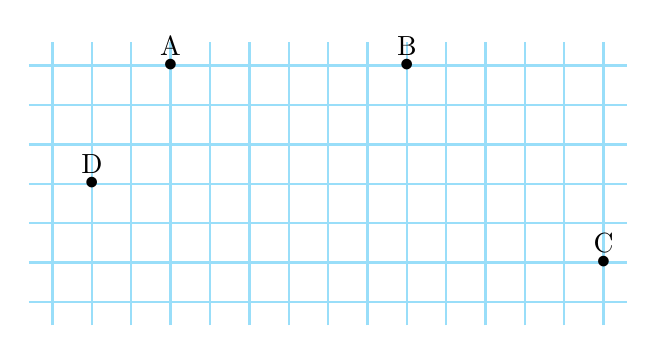
\begin{tikzpicture}
 \draw[quadrillage55] (-.8,-.8)grid(6.8,2.8) ;
 \draw (1,2.5) node[above]{A};
 \draw (1,2.5) node {$\bullet$};
 \draw (4,2.5) node[above]{B};
 \draw (4,2.5) node {$\bullet$};
 \draw (6.5,0) node[above]{C};
 \draw (6.5,0) node {$\bullet$};
 \draw (0,1) node[above]{D};
 \draw (0,1) node {$\bullet$};
 \end{tikzpicture}
\end{center}
 \begin{enumerate}
  \item En utilisant le quadrillage de ton cahier, place les points $A$, $B$, $C$ et $D$ comme sur la figure ci-dessus;
  \item Trace en bleu le segment $[AB]$ ;
  \item Trace en vert le segment d'extrémités $D$ et $C$ ;
  \item Trace en rouge la droite passant par $A$ et $C$ ;
  \item Trace en noir la demi-droite d'origine $D$ passant par $B$.
  \end{enumerate}
 \end{exercice}


\begin{exercice}[Appartient ou pas ?]
 \begin{center} 
\begin{tikzpicture}[rotate=20]
\draw (1,0) node[below right]{A};
 \draw (1,0) node[rotate=20] {$|$};
 \draw (2.5,0) node[below right]{B};
 \draw (2.5,0) node[rotate=20] {$|$};
 \draw (5,0) node[below right]{C};
 \draw (5,0) node[rotate=20] {$|$};
 \draw (5.7,0) node[below right]{D};
 \draw (5.7,0) node[rotate=20] {$|$};
  \draw (4,1.2) node[above left]{E};
 \draw (4,1.2) node {$\times$};
 \draw(0,0)--(6.5,0);
\end{tikzpicture} 
 \end{center}
 Après avoir observé la figure, recopie et complète les pointillés avec $\in$ ou $\notin$ :
    \begin{colenumerate}{3}
     \item $B$ \ldots $[AC]$ ;
     \item $D$ \ldots $[AB]$ ;
     \item $E$ \ldots $[AD]$ ;
     \item $B$ \ldots $[CA)$ ;
     \item $D$ \ldots $[CA)$ ;
     \item $E$ \ldots $[CE]$.
     \end{colenumerate}
\end{exercice}


\begin{exercice}[À trouver]
 \begin{center}
 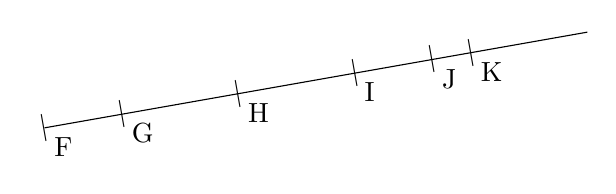
\begin{tikzpicture}[rotate=10]
\draw (0,0) node[below right]{F};
 \draw (0,0) node[rotate=10] {$|$};
 \draw (1,0) node[below right]{G};
 \draw (1,0) node[rotate=10] {$|$};
 \draw (2.5,0) node[below right]{H};
 \draw (2.5,0) node[rotate=10] {$|$};
 \draw (4,0) node[below right]{I};
 \draw (4,0) node[rotate=10] {$|$};
 \draw (5,0) node[below right]{J};
 \draw (5,0) node[rotate=10] {$|$};
 \draw (5.5,0) node[below right]{K};
 \draw (5.5,0) node[rotate=10] {$|$};
 \draw(0,0)--(7,0);
\end{tikzpicture} 
\end{center}
 Parmi les points nommés sur la figure, indique ceux qui appartiennent à :
    \begin{colenumerate}{2}
     \item $[FK]$ ;
     \item $[IG)$ ;
     \item $[FJ]$ et à $[GK]$ ;
     \item $[GJ)$ mais pas à $[HJ]$ ;
     \item $[FG]$ ou à $[IJ)$ ;
     \item $[FH]$ et à $[JK]$.
     \end{colenumerate}
\end{exercice}


\begin{exercice}[Vrai ou faux ?]
 \begin{center} 
 \begin{tikzpicture}[scale=0.8]
 \draw (0,0) node[above]{A}--+(90:0.08)--+(-90:0.08);
 \draw (0,0)--(2,0) node[above right]{M}--++(120:2) node[above]{C}--+(30:0.08)--+(210:0.08);
\path (0,0)--(2,0) node[midway,blue,rotate=-15]{$||$};
\path (2,0)--++(120:2) node[midway,blue,rotate=-15]{$||$};
\draw (2,0)--++(-60:2)node[right]{D}--+(30:0.08)--+(210:0.08);
\path (2,0)--++(-60:2) node[midway,blue,rotate=-15]{$||$};
\draw(2,0)--(6,0)node[above]{B}--+(90:0.08)--+(-90:0.08);
 \end{tikzpicture}
 \end{center}
 Observe cette figure composée de deux segments $[AB]$ et $[CD]$ sécants et indique pour chaque affirmation si elle est vraie ou fausse :
 \begin{enumerate}
  \item Les points $C$, $D$ et $M$ sont alignés ;
  \item $M$ est le point d'intersection de $[AB]$ et $[CD]$ ;
  \item $M$ est le milieu du segment $[AC]$ ;
  \item $M$ est un point du segment $[CD]$ ;
  \item $A$ appartient au segment $[MB]$ ;
  \item $M$ est le milieu du segment $[CD]$.
 \end{enumerate}
\end{exercice}


\begin{exercice}[Milieux]
\begin{enumerate} 
 \item Trace un segment $[RS]$ de longueur 4,8 cm et place son milieu $T$ ;
 \item Place un point $U$ qui ne soit pas aligné avec $R$ et $S$ ;
 \item Place le point $V$ tel que $T$ soit le milieu de $[UV]$.
 \end{enumerate}
\end{exercice}


\begin{exercice}[À construire]
\begin{enumerate} 
 \item Place trois points $A$, $B$ et $C$ non alignés ;
 \item Trace les segments $[BC]$ et $[AC]$ ;
 \item Marque le milieu $I$ du segment $[BC]$ et le milieu $J$ du segment $[AC]$ ;
 \item Trace le segment d'extrémités $B$ et $J$ ;
 \item Note $K$ le point d'intersection de $[AI]$ et $[BJ]$ ;
 \item Trace le segment $[AB]$ et place son milieu $L$. Trace enfin le segment $[CL]$. Que remarques‑tu ?
 \end{enumerate}
\end{exercice}


\begin{exercice}[À construire (bis)]
\begin{enumerate} 
 \item Place trois points $L$, $M$ et $N$ non alignés ;
 \item Place un point $A$ appartenant au segment $[LN]$ ;
 \item Place un point $B$ appartenant à la demi‑droite $[MN)$ mais n'appartenant pas au segment $[MN]$ ;
 \item Place le point $C$ aligné d'une part avec $A$ et $B$, et d'autre part avec $L$ et $M$.
 \end{enumerate}
\end{exercice}



%%%%%%%%%%%%%%%%%%%%Mise en page
\vspace{1em}
%%%%%%%%%%%%%%%%%%%%%%%%%%%%%%%



\begin{exercice}[Bande dessinée]
 \begin{center}
  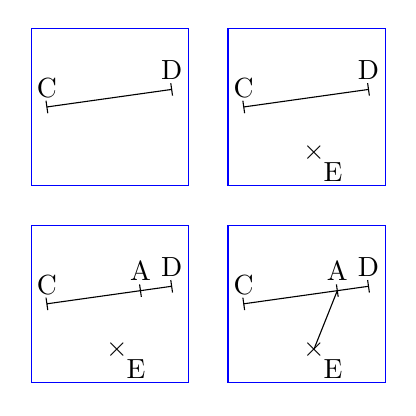
\begin{tikzpicture}
%rectangle 1 (haut à gauche)
 \draw [blue](0,2.5) rectangle (2,4.5);
 \begin{scope}[shift={(0.2,3.5)},rotate=8]
 \draw (0,0) node [above]{C}--+(+90:0.08)--+(-90:0.08);
 \draw(0,0)--++(1.6,0) node [above]{D}--+(90:0.08)--+(-90:0.08);
 \end{scope}
 %rectangle 2 (haut droite)
 \draw [blue](2.5,2.5) rectangle (4.5,4.5);
  \begin{scope}[shift={(2.7,3.5)},rotate=8]
 \draw (0,0) node [above]{C}--+(+90:0.08)--+(-90:0.08)--(0,0)--(1.6,0) node [above]{D}--+(90:0.08)--+(-90:0.08);
  \draw (0.8,-0.7) node [below right]{E};
 \draw (0.8,-0.7) node {$\times$};
 \end{scope}
 %rectangle 3 (bas gauche)
  \draw [blue](0,0) rectangle (2,2);
  \begin{scope}[shift={(0.2,1)},rotate=8]
 \draw (0,0) node [above]{C}--+(+90:0.08)--+(-90:0.08)--(0,0)--(1.6,0) node [above]{D}--+(90:0.08)--+(-90:0.08);
  \draw (0.8,-0.7) node [below right]{E};
 \draw (0.8,-0.7) node {$\times$};
 \draw (1.2,0) node [above]{A}--+(+90:0.08)--+(-90:0.08);
 \end{scope}
 %rectangle 4 (bas droite)
 \draw [blue](2.5,0) rectangle (4.5,2);
  \begin{scope}[shift={(2.7,1)},rotate=8]
 \draw (0,0) node [above]{C}--+(+90:0.08)--+(-90:0.08)--(0,0)--(1.6,0) node [above]{D}--+(90:0.08)--+(-90:0.08);
  \draw (0.8,-0.7) node [below right]{E};
 \draw (0.8,-0.7) node {$\times$};
 \draw (1.2,0) node [above]{A}--+(+90:0.08)--+(-90:0.08);
 \draw (1.2,0)--(0.8,-0.7);
 \end{scope}
 \end{tikzpicture}
\end{center}
Pour chaque étape de la bande dessinée, écris la consigne qui a été donnée, sans tenir compte des mesures.
\end{exercice}

%%%%%%%%%%%%%%%%%%%%%%%%%%%%%%%%%%%%%%%%%%%%%%%%%%%%%%%%%

\serie{Droites parallèles et perpendiculaires}

\begin{exercice}[Position de droites]
 \begin{center}
 \includegraphics[width=5.8cm]{mikado}  \end{center}
Observe la figure ci‑dessus et note sur ton cahier :
\begin{itemize}
 \item Le nom des droites qui \textbf{te semblent} perpendiculaires ;
 \item Le nom des droites qui sont sécantes mais non perpendiculaires ;
 \item Le nom des droites qui \textbf{te semblent} parallèles.
 \end{itemize}
\end{exercice}


\begin{exercice}[Position de droites (bis)]
 \begin{center} \includegraphics[width=7.3cm]{mikado2}  \end{center}
\begin{enumerate}
 \item Quelles sont les droites qui sont à coup sûr perpendiculaires ?
 \item Quelle semble être la position relative des droites $(BA)$ et $(GR)$ ?
 \end{enumerate}
\end{exercice}


\begin{exercice}[Quadrillage]
Sur la figure ci-dessous, trace, à la règle, la droite $d_1$ perpendiculaire à la droite $d$ passant par le point $M$ et la droite $d_2$ parallèle à la droite $d'$ passant par $M$.
\begin{center}
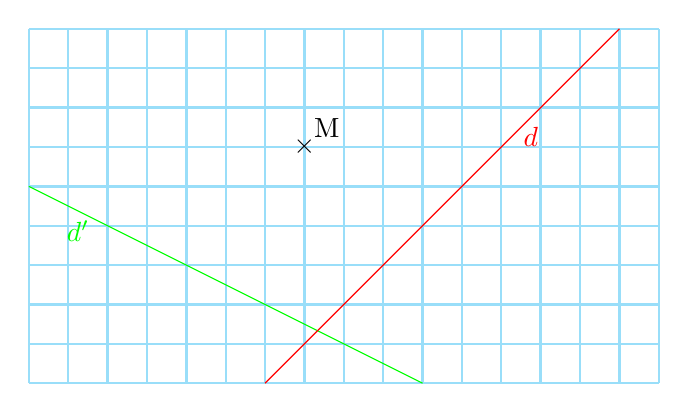
\begin{tikzpicture}
\draw[quadrillage55](0,0) grid (8,4.5);
\draw [green](0,2.5)--(5,0) node[very near start,below,green]{$d'$};
\draw[red] (3,0)--(7.5,4.5) node[near end,below,red]{$d$};
\draw(3.5,3) node[above right] {M};
\draw (3.5,3) node {$\times$};
\end{tikzpicture}
\end{center}
\end{exercice}


\begin{exercice}[Constructions]
\begin{enumerate}
 \item Reproduis sur une feuille blanche les deux figures ci‑dessous :
 \begin{center} \includegraphics[width=6.1cm]{constructions}  \end{center}
 \item Pour chacune des figures, trace :
  \begin{itemize}
   \item La droite $d'$ perpendiculaire à $d$ et passant par $B$ ;
   \item La droite $d''$ perpendiculaire à $d$ et passant par $A$.
   \end{itemize}
 \item Que peux‑tu dire des droites $d'$ et $d''$ ?
 \end{enumerate}
\end{exercice}


\begin{exercice}[Constructions (bis)]
 \begin{center}
 \begin{tikzpicture}[rotate=10]
 \draw (0.0)--(6,0) node[very near start,below]{$d$};
 \draw (1,1) node[left]{A};
 \draw (1,1) node{$\times$};
 \draw (5,-1) node[left]{B};
 \draw (5,-1) node{$\times$};
 \end{tikzpicture}
\end{center}
\begin{enumerate}
 \item Reproduis la figure ci‑dessus ;
 \item Trace $d'$, la parallèle à $d$ passant par $A$ ;
 \item Trace $d''$, la parallèle à $d$ passant par $B$ ;
 \item Que peux‑tu dire des droites $d'$ et $d''$ ?
 \end{enumerate}
\end{exercice}


%%%%%%%%%%%%%%%%%%%%Mise en page
\newpage
%%%%%%%%%%%%%%%%%%%%%%%%%%%%%%%



\begin{exercice}[Programme de construction]
\begin{enumerate}
 \item Place deux points $A$ et $B$ tels que $AB = 8$ cm ;
 \item Place un point $L$ sur $[AB]$ tel que $AL = 3$ cm ;
 \item Trace la droite $d$ telle que $L \in d$ et $(AB) \perp d$ ;
 \item Place un point $C$ tel que $C \in d$ et $LC = 2$ cm ;
 \item Trace la droite $d'$ telle que $d' \parallel (AB)$ et $C \in d'$ ;
 \item Sur la demi‑droite $[BC)$, place le point $I$ tel que $BI = 7$ cm ;
 \item Trace la droite $d''$ telle que $I \in d''$ et $d'' \parallel (AC)$.
 \end{enumerate}
\end{exercice}


\begin{exercice}
Construis la figure suivante : \\[0.75em]
\begin{minipage}[c]{0.2\textwidth}
\includegraphics[width=3.8cm]{constructions3}
 \end{minipage} \hfill%
 \begin{minipage}[c]{0.2\textwidth}
 $(BM) \parallel (AN)$
  \end{minipage} \\
\end{exercice}


\begin{exercice}
Reproduis la figure ci‑dessous en vraie grandeur : \\[0.75em]
\begin{minipage}[c]{0.3\textwidth}
\includegraphics[width=4.5cm]{double-triangle}
 \end{minipage} \hfill%
 \begin{minipage}[c]{0.4\textwidth}
$AB = 5,3$ cm ;

$BC = 3$ cm ;

$AC = 7,7$ cm.
 \end{minipage} \\
\end{exercice}

%%%%%%%%%%%%%%%%%%%%%%%%%%%%%%%%%%%%%%%%%%%%%%%%%%%%%%%%%

\serie{Médiatrice d’un segment}

\begin{exercice}[Médiatrices]
Dans chaque cas, trace le segment de longueur donnée puis sa médiatrice :
 \begin{colenumerate}{3}
  \item $AB = 2$ cm ;
  \item $DE = 7,8$ cm ;
  \item $FG = 76$ mm.
  \end{colenumerate}
\end{exercice}


\begin{exercice}[Points alignés]
 \begin{enumerate}
  \item Trace un segment $[AB]$ de longueur 7 cm ;
  \item Place le point $C$ de la demi‑droite $[BA)$ tel que $BC = 12$ cm ;
  \item Construis la médiatrice $m_1$ du segment $[AC]$ ;
  \item Construis la médiatrice $m_2$ du segment $[AB]$ ;
  \item Que remarques‑tu ?
  \end{enumerate}
\end{exercice}


\begin{exercice}[Reconnaître]
Sur chacune des figures ci‑dessous, indique si $P$ est sur la médiatrice de $[AB]$ : \\[0.5em]
 \begin{colenumerate}{2}
  \item \\
  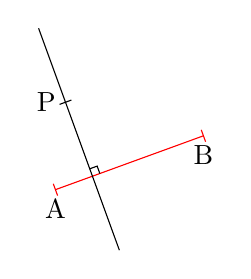
\begin{tikzpicture}[rotate=20]
 \draw[red] (0,0) node[below,black]{A}-- +(90:0.08)-- +(-90:0.08)--(0,0)--(2,0) node [below,black]{B}--+(90:0.08)--+(-90:0.08);
 \draw (0.5,0.1)-|(0.6,0);
  \draw (0.5,-1)--(0.5,1) node [left]{P}--+(0:0.08)--+(180:0.08)--(0.5,1)--(0.5,2);
  \end{tikzpicture}
  \item \\
    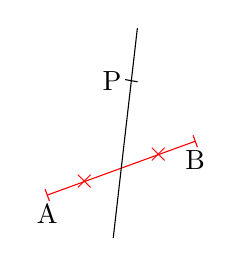
\begin{tikzpicture}[rotate=20]
 \draw[red] (0,0) node[below,black]{A}-- +(90:0.08)-- +(-90:0.08)--(0,0)--(1,0) node[midway]{$\times$}--(2,0) node [midway]{$\times$}--+(90:0.08)--+(-90:0.08);
 \draw (2,0) node [below]{B};
 \draw (1.5,1) node [left]{P}--+(-30:0.08)--+(150:0.08);
 \draw (0.6,-0.8)--(1.8,1.6);
    \end{tikzpicture}
  \item \\
 \begin{tikzpicture}[scale=0.8]
\draw[red] (0,0)--(1,2) node[midway,black]{$\times$};
 \draw (1,2) --(3,1) node[midway]{$\times$}--(0,0);
 \draw (0,0) node[below left]{A};
 \draw (1,2) node[above]{B};
 \draw (3,1) node[right]{P};
 \end{tikzpicture} 

  \item \\
 \begin{tikzpicture}[scale=0.8]
\draw[red] (0,0)--(3,1);
 \draw (0,0) --(1,2) node[midway]{$\times$}--(3,1)node[midway]{$\times$};
 \draw (0,0) node[below left]{A};
 \draw (1,2) node[above]{P};
 \draw (3,1) node[right]{B};
 \end{tikzpicture}
  \end{colenumerate}
\end{exercice}
 
 
\begin{exercice}[Construction]
 \begin{enumerate}
 \item Trace un segment $[AB]$ de longueur 6 cm ;
 \item Construis la médiatrice $d$ du segment $[AB]$ au compas ;
 \item Place un point $M$ sur $d$ à 7 cm de $A$ ;
 \item Quelle est la longueur de $[BM]$ ? 
 
Tu la justifieras en utilisant une propriété.
  \end{enumerate}
\end{exercice}


\begin{exercice}[Concours de médiatrices]
 \begin{enumerate}
 \item Place trois points $A$, $B$ et $C$ non alignés ;
 \item Trace sans équerre les médiatrices des segments $[AB]$, $[AC]$ et $[BC]$. 
 
 Que constates‑tu ?
 \end{enumerate}
\end{exercice}


%%%%%%%%%%%%%%%%%%%%Mise en page
\newpage
%%%%%%%%%%%%%%%%%%%%%%%%%%%%%%%



%%%%%%%%%%%%%%%%%%%%%%%%%%%%%%%%%%%%%%%%%%%%%%%%%%%%%%%%%

\serie{Nommer un angle}


\begin{exercice}[De toutes les couleurs]
Les points $A$, $O$ et $L$ sont alignés.
 \begin{center} \includegraphics[width=6.7cm]{angles-colores}  \end{center}
\begin{enumerate}
 \item Nomme les angles marqués en couleur dans la figure de toutes les façons possibles ; 
 \item Reproduis la figure puis marque en bleu l'angle $\widehat{yOz}$, en rouge l'angle $\widehat{PMC}$ et en vert l'angle $\widehat{PAL}$.
 \end{enumerate}
\end{exercice}


\begin{exercice}[Plusieurs noms]
Les segments $[TD]$ et $[PS]$ sont sécants en $A$ et les segments $[PI]$ et $[TD]$ se coupent en $R$.

Trouve toutes les autres façons de nommer : \\[0.5em]
\begin{minipage}[c]{0.2\textwidth}
\begin{itemize}
 \item l'angle $\widehat{APR}$ ;
 \item l'angle $\widehat{RDI}$ ;
 \item l'angle $\widehat{PDA}$.
 \end{itemize}
 \end{minipage} \hfill%
  \begin{minipage}[c]{0.4\textwidth}
  \includegraphics[width=4.7cm]{segments-secants}
  \end{minipage} \\
\end{exercice}  


\begin{exercice}[Quelle étourdie !]
Louise a recopié la figure ci‑dessous qui était au tableau mais elle a oublié de noter les noms des points d'intersection des droites. 
 \begin{center} \includegraphics[width=5.2cm]{angles-multicolores}  \end{center}
Elle appelle son camarade Ahmed qui lui dit que les angles en couleur se nomment $\widehat{ABC}$, $\widehat{DBA}$, $\widehat{FAC}$ et $\widehat{FAE}$. \\[0.5em]
Reproduis la figure et nomme les points grâce à ces indications.
\end{exercice}  


%%%%%%%%%%%%%%%%%%%%Mise en page
\vspace{3em}
%%%%%%%%%%%%%%%%%%%%%%%%%%%%%%%




%%%%%%%%%%%%%%%%%%%%%%%%%%%%%%%%%%%%%%%%%%%%%%%%%%%%%%%%%

\serie{Mesure d'un angle}


\begin{exercice}[À vue d’œil]
\prof
{ce travail sera fait de façon approximative; il peut être sujet à discussion.}

Indique les angles qui te paraissent obtus, aigus ou droits.
 \begin{center} \includegraphics[width=7cm]{angles-toutgenre}  \end{center}
\end{exercice}


\begin{exercice}[Avec l'équerre]
\prof
{Ce travail sera fait de façon approximative; il peut être sujet à discussion.}

En utilisant ton équerre, détermine quels sont les angles aigus, obtus ou droits dans chacun des cas ci-dessous.
 \begin{center} \includegraphics[width=7cm]{angles-droits}  \end{center}
\end{exercice}

%%%%%%%%%%%%%%%%%%%%Mise en page
\newpage
%%%%%%%%%%%%%%%%%%%%%%%%%%%%%%%

\begin{exercice}[Bien placé ?]
Dans chacun des cas suivants, José souhaite mesurer l'angle $\widehat{BAC}$.

Peut‑il effectuer une mesure correcte ? Si oui, indique la mesure de l'angle et si non, explique pourquoi. \\[0.5em]
\begin{colenumerate}{1}
 \item \\
 \begin{center}\input{./PointsSegmentsDroites/figures/BienPlace_Fig1}\end{center}
\item \\
 \begin{center}\input{./PointsSegmentsDroites/figures/BienPlace_Fig2}\end{center}
 \item \\
  \begin{center}\input{./PointsSegmentsDroites/figures/BienPlace_Fig3}\end{center}
 \item \\
\begin{center}\input{./PointsSegmentsDroites/figures/BienPlace_Fig4}\end{center}
 \item \\
\begin{center}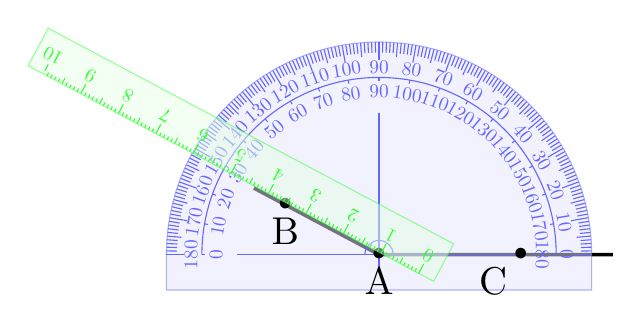
\begin{tikzpicture}[scale=.9]

\def \RotFigure {0} %rotation de toute la figure y compris textes
\begin{scope}[rotate=\RotFigure]

\def \CharSize {1.4};
\def \BulletSize {1};
\coordinate (A) at (0,0);
\coordinate (B) at (-1.324,0.704);
\coordinate (C) at (2,0);
\coordinate (U) at (-1.766,0.939);
\coordinate (V) at (3.3,0);

\draw[line width = 1.3pt] (U) -- (A) -- (V);
	
%début du rapporteur
    %Définition de l 'angle de rotation du rapporteur
    \def \Rotation {0} 
    %Définition du décalage du rapporteur
    \def \DecalX {0}
    \def \DecalY {0}
    %Couleur des élèments du rapporteur (sauf le remplissage)
    \def \RapColor {blue!60}

\begin{scope}[shift={(\DecalX,\DecalY)},rotate=\Rotation]
    % contours du rapporteur
    \draw[color=\RapColor, fill =blue!10, opacity=0.5] (-3,0) arc(180:0:3)--(3,-0.5)--(-3,-0.5)--cycle;	%Dont couleur de remplissage
    \draw[color=\RapColor] (-2,0)--(2,0);
    \draw[color=\RapColor] (0,-0.2)--(0,2);
    % graduation externe 1 degrés
    \foreach \a in {0,1,...,180}{\draw[color=\RapColor] (\a:3)--(\a:2.85);}
    % graduation externe 5 degrés
    \foreach \a in {0,5,...,180}{\draw[color=\RapColor] (\a:2.85)--(\a:2.8);}
    % double graduation
   \foreach \a/\b in {%
        0/-90,10/-80,20/-70,30/-60,40/-50,50/-40,%
        60/-30,70/-20,80/-10,90/0,100/10,110/20,%
        120/30,130/40,140/50,150/60,160/70,170/80,180/90%
    }{
    % graduation externe 10 degrés
    \draw[color=\RapColor] (\a:2.80)--(\a:2.75) 
    node[scale=0.7, rotate=\b+\Rotation+\RotFigure] (\a) at (\a:2.65){\a};
    % graduation interne 10 degrés
    \draw[color=\RapColor] (\a:2.5)--(\a:2.45)
	node[thin,scale=0.7, rotate=-\b+\Rotation+\RotFigure] (\a) at (180-\a:2.3){\a}; }
    % demi-cercle intérieur
    \draw[color=\RapColor](-2.5,0) arc(180:0:2.5);
    %demi-cercle à l'origine
    \draw[color=\RapColor](-0.2,0) arc(180:0:0.2);
\end{scope}
%fin du rapporteur

\draw (A) node [below,scale=\CharSize,rotate=\RotFigure]{A};
\draw (A) node[scale=\BulletSize]{$\bullet$};
\draw (B) node [below,scale=\CharSize,rotate=\RotFigure]{B};
\draw (B) node[scale=\BulletSize]{$\bullet$};
\draw (C) node [below left,scale=\CharSize,rotate=\RotFigure]{C};
\draw (C) node[scale=\BulletSize]{$\bullet$};

	
%début de la règle
    %Graduaton max. de la règle
    \def \TailleRegle {10}
    %Définition de l 'angle de rotation de la règle
    \def \RotationRegle {152}
    %Définition du décalage de la règle
    \def \DecalRegleX {0.7}
    \def \DecalRegleY {0}
    %Couleur des élèments de la règle (sauf le remplissage)
    \def \RegleColor {green!80}

\begin{scope}[shift={(\DecalRegleX,\DecalRegleY)},rotate=\RotationRegle, scale=0.6]
    % contours de la règle
    \draw[color=\RegleColor, fill =green!10, opacity=0.5] (-0.4,0.5) rectangle (\TailleRegle+0.4,-0.5);	%Dont couleur de remplissage
    % graduation 1 mm
    \foreach \a in {0,0.1,...,\TailleRegle}{\draw[color=\RegleColor] (\a,0.5)--(\a,0.42);}
    % graduation 5 mm
    \foreach \a in {0,0.5,...,\TailleRegle}{\draw[color=\RegleColor] (\a,0.42)--(\a,0.35);}
    % graduation et repères 10 mm
    \foreach \a in {0,1,...,\TailleRegle}{\draw[color=\RegleColor] (\a,0.35)--(\a,0.25)
    node[scale=0.7, rotate=\RotationRegle+\RotFigure] (\a) at (\a,0.02){\a};}
    
\end{scope}
%fin de la règle

\end{scope}
\end{tikzpicture}\end{center}
 \item \\
\begin{center}\input{./PointsSegmentsDroites/figures/BienPlace_Fig6}\end{center}
 \end{colenumerate}
\end{exercice}  


\begin{exercice}[Alignés ?]
Dans la figure ci-dessous faite à main levée, on donne : $\widehat{LIS}= 44^\circ$.
Les points $F$, $I$ et $L$ sont-ils alignés ? Justifie.
 \begin{center} \includegraphics[width=4.2cm]{croquis-tordu} \end{center}
\end{exercice} 



\begin{exercice}[Quelle échelle ?]
Pour chaque angle, indique s'il est aigu ou obtus. Note ensuite sa mesure sur la bonne graduation du rapporteur.
\begin{colenumerate}{2}
 \item  
 
 \includegraphics[width=3.3cm]{rapporteur-bleu}
 \item 
 
 \includegraphics[width=3.2cm]{rapporteur-vert}
 \item 

 \includegraphics[width=3.1cm]{rapporteur-rose}
 \item 
 
 \includegraphics[width=3.3cm]{rapporteur-orange}
 
 \end{colenumerate}
\end{exercice} 

\begin{exercice}
Mesure les angles ci‑dessous avec ton rapporteur.
 \begin{center} \includegraphics[width=4cm]{angles-rose-vert} \end{center}
 
 \begin{center} \includegraphics[width=4cm]{angles-gris} \end{center}
\end{exercice} 




%%%%%%%%%%%%%%%%%%%%Mise en page
\newpage
%%%%%%%%%%%%%%%%%%%%%%%%%%%%%%%



%%%%%%%%%%%%%%%%%%%%%%%%%%%%%%%%%%%%%%%%%%%%%%%%%%%%%%%%%

\serie{Construire un angle}

\begin{exercice}
Construis les angles suivants :

$\widehat{MOT} = 27^\circ$ ; $\widehat{SUD} = 151^\circ$ ; $\widehat{FIN} = 47^\circ$ et $\widehat{PRE} = 110^\circ$.
\end{exercice} 


\begin{exercice}[Programme de construction]
\begin{enumerate}
\item Trace $[AC]$ tel que $AC = 3$ cm. Construis un angle $\widehat{ACx}$ mesurant $60^\circ$. Place un point $B$ sur $[Cx)$ tel que $CB = 5,6$ cm ;
\item Place le point $D$ sur $[AB]$ tel que $\widehat{DCB} = 25^\circ$ ;
\item Place le point $E$ sur $[AD]$ tel que $\widehat{DCE} = 25^\circ$.
\end{enumerate}
\end{exercice} 


\begin{exercice}[Secteur angulaire]
Voici une figure construite par Joséphine. Reproduis la figure sur ton cahier.
 \begin{center} \includegraphics[width=4.7cm]{secteurABCDE} \end{center}
\end{exercice} 


\begin{exercice}[Reproduction de figure]
 \begin{center} \includegraphics[width=4.2cm]{croquisAPCTR} \end{center}
 Voici le croquis d’une figure dans laquelle les points $A$, $R$ et $T$ sont alignés. Construis la figure.
\end{exercice} 


%%%%%%%%%%%%%%%%%%%%%%%%%%%%%%%%%%%Mise en page
\columnbreak
%%%%%%%%%%%%%%%%%%%%%%%%%%%%%%%%%%%%%%%%%%%%%%


%%%%%%%%%%%%%%%%%%%%%%%%%%%%%%%%%%%%%%%%%%%%%%%%%%%%%%%%%

\serie{Bissectrice d'un angle}

\begin{exercice}[Reconnaître]
Pour quelle(s) figure(s) la demi‑droite rouge semble être la bissectrice de l'angle ?
\begin{colenumerate}{3}
 \item  \\
  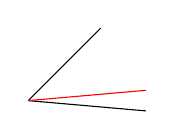
\begin{tikzpicture}
 \draw (0,0)--+(-5:1.5);
 \draw (0,0)--+(45:1.3);
 \draw [red] (0,0)--(5:1.5);
 \end{tikzpicture}

 \item  \\
  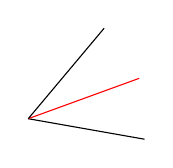
\begin{tikzpicture}
 \draw (0,0)--+(-10:1.5);
 \draw [red](0,0)--+(20:1.5);
 \draw (0,0)--(50:1.5);
 \end{tikzpicture}

 \item   \\
  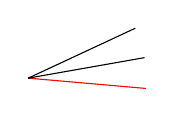
\begin{tikzpicture}
 \draw [red] (0,0)--+(-5:1.5);
 \draw (0,0)--+(10:1.5);
 \draw (0,0)--(25:1.5);
 \end{tikzpicture}
  
 \item  \\
  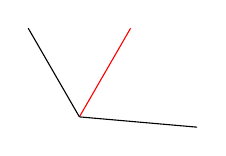
\begin{tikzpicture}
 \draw (0,0)--+(-5:1.5);
 \draw [red](0,0)--+(60:1.3);
 \draw (0,0)--(120:1.3);
 \end{tikzpicture}
 
 \item \\
  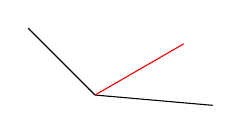
\begin{tikzpicture}
 \draw (0,0)--+(-5:1.5);
 \draw [red](0,0)--+(30:1.3);
 \draw (0,0)--(135:1.2);
 \end{tikzpicture}

 \end{colenumerate}
\end{exercice} 


\begin{exercice}[Bissectrice et construction]
Dans chaque cas, trace un angle dont la mesure est donnée puis construis sa bissectrice au compas :
\begin{colenumerate}{3}
 \item $\widehat{ABC} = 32^\circ$ ;
  \item $\widehat{UST} = 180^\circ$ ; 
  \item $\widehat{ZXY} = 67^\circ$ ;
  \item $\widehat{WZD} = 90^\circ$ ;
  \item $\widehat{PRT} = 127^\circ$ ;
  \item $\widehat{LKI} = 154^\circ$.
 \end{colenumerate}
\end{exercice} 


\begin{exercice}[Mesure d'angles]
\begin{enumerate}
 \item Trace un angle $\widehat{EDF}$ qui mesure $28^\circ$ ; \label{PtSegDr_entrain_mesangl_a}
 \item Construis la bissectrice de $\widehat{EDF}$ et place un point $G$ sur celle‑ci ;
 \item Calcule la mesure de l'angle $\widehat{GDF}$. Justifie ; \label{PtSegDr_entrain_mesangl_c}
 \item Recommence les questions de \ref{PtSegDr_entrain_mesangl_a} à \ref{PtSegDr_entrain_mesangl_c} avec un angle de $133^\circ$.
 \end{enumerate}
\end{exercice} 


%%%%%%%%%%%%%%%%%%%%%%%%%%%%%%%%%%%Mise en page

\vspace*{3cm}

\phantom{coucou}

\pagebreak
%%%%%%%%%%%%%%%%%%%%%%%%%%%%%%%%%%%%%%%%%%%%%%


%%%%%%%%%%%%%%%%%%%%%%%%%%%%%%%%%%%%%%%%%%%%%%%%%%%%%%%%%

\serie{Cercle}

\begin{exercice}[Vocabulaire]
 \begin{center}
 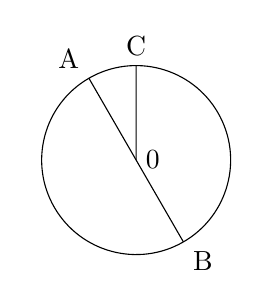
\begin{tikzpicture}[rotate=-60]
 \draw (0,0) circle(1.2) node[right]{0};
 \draw (-1.2,0) node [above left]{A}--(1.2,0) node [below right]{B};
 \draw (0,0)--(150:1.2) node[above]{C};
 \end{tikzpicture}
 \end{center}
 Sur la figure ci-dessus : 
 
$A$, $B$ et $C$ sont sur le cercle de centre $O$ ;

$A$, $O$ et $B$ sont alignés.
 \begin{enumerate}
  \item Écris deux phrases décrivant la figure, en utilisant les mots « rayon » et « diamètre » ;
  \item Complète les phrases suivantes :
   \begin{itemize}
    \item Le point $O$ est le milieu du \dotfill ;
    \item Le point $O$ est une extrémité du \dotfill ;
    \item $A$ et $B$ sont les \dotfill du \dotfill $[AB]$ ;
    \item La portion de cercle comprise entre les points $A$ et $C$ est l'\dotfill.
    \end{itemize}
  \end{enumerate}
\end{exercice}


\begin{exercice}[Avec le rayon]
Trace un cercle de centre $O$ et de rayon 4 cm puis un cercle de rayon 4 cm et passant par $O$.
\end{exercice}


\begin{exercice}[Avec le diamètre]
 \begin{enumerate}
  \item Trace un segment $[AB]$ de longueur 5 cm ;
  \item Trace le cercle de diamètre $[AB]$ ;
  \item Quelle est la mesure du rayon de ce cercle ?
  \end{enumerate}
\end{exercice}



\begin{exercice}[Construction]
 \begin{enumerate}
  \item Trace un cercle $(\mathcal{C})$ de centre $O$ et de rayon 4,5 cm ;
  \item Place un point $A$ sur le cercle $(\mathcal{C})$ et place le point $B$ diamétralement opposé au point $A$ ;
  \item Marque un point $D$ à l'extérieur du cercle $(\mathcal{C})$ et trace le cercle de diamètre $[BD]$.
 \end{enumerate}
\end{exercice}



\begin{exercice}[Calculs]
 \begin{enumerate}
  \item Trace un segment $[AB]$ de longueur 6 cm. Trace le cercle de centre $A$ et de rayon 2 cm. Ce cercle coupe la droite $(AB)$ en deux points $M$ et $N$. On appelle $M$ celui qui appartient au segment $[AB]$ ;
  \item Calcule les longueurs $BM$ et $BN$.
 \end{enumerate}
\end{exercice}


\begin{exercice}[Concentriques]
Deux cercles concentriques (c'est‑à‑dire de même centre) $(\mathcal{C})$ et $(\mathcal{C’})$ ont pour centre $O$ et pour rayons respectifs 3 cm et 5 cm. $[GH]$ est un diamètre du cercle $(\mathcal{C})$. 

La droite passant par $G$ et par $H$ coupe le cercle $(\mathcal{C'})$ en deux points $I$ et $J$ ; on appelle $I$ celui qui est le plus près de $G$.
\begin{enumerate}
  \item Fais une figure ;
  \item Calcule les longueurs $GI$ et $JG$.
 \end{enumerate}
\end{exercice}


\begin{exercice}[Calculs]
\begin{enumerate}
  \item Trace un segment $[ST]$ de longueur 6 cm. Sur ce segment, marque le point $U$ tel que $SU = 3,2$ cm. Trace le cercle $(\mathcal{C})$ de centre $T$ et qui passe par $U$ ;
  \item Calcule le diamètre du cercle $(\mathcal{C})$ ;
  \item Sur le segment $[UT]$, place le point $V$ tel que $UV = 1,2$ cm. Quel est le rayon du cercle de diamètre $[SV]$ ?
 \end{enumerate}
\end{exercice}


\begin{exercice}
Construis la figure ci-dessous donnée par son croquis.

\begin{center} \includegraphics[width=3.4cm]{double-cercle} \end{center}
\end{exercice}


%%%%%%%%%%%%%%%%%%%%%%%%%%%%%%%%%%%Mise en page

\vspace*{3cm}

\phantom{coucou}

\pagebreak
%%%%%%%%%%%%%%%%%%%%%%%%%%%%%%%%%%%%%%%%%%%%%%



\begin{exercice}
Construis chaque figure ci-dessous donnée par son croquis.
\begin{colenumerate}{2}
 \item
 
 \includegraphics[width=3.9cm]{4cercles}
 \item
 
\includegraphics[width=2.6cm]{goutte-rose}
 \item
 
\includegraphics[width=4cm]{theatre}
 \end{colenumerate}
\end{exercice}


\begin{exercice}
En utilisant le quadrillage de ton cahier, reproduis les figures suivantes.
\begin{colenumerate}{2}
 \item
 
 \includegraphics[width=2.9cm]{quadrillage-cercles}
 \item
 
\includegraphics[width=3.1cm]{quadrillage-parap}

 \end{colenumerate}
\end{exercice}


\begin{exercice}[À construire]
\begin{enumerate}
 \item Trace un segment $[AB]$ de longueur 6 cm ;
 \item Marque le point $O$, milieu du segment $[AB]$ ;
 \item Trace le cercle de centre $O$ et de rayon 3 cm ;
 \item Trace les cercles de diamètres $[AO]$ et $[OB]$.
 \end{enumerate}
\end{exercice}



%%%%%%%%%%%%%%%%%%%%%%%%%%%%%%%%%%%Mise en page
\columnbreak
%%%%%%%%%%%%%%%%%%%%%%%%%%%%%%%%%%%%%%%%%%%%%%


\begin{exercice}[À construire (bis)]
\begin{enumerate}
 \item Trace un segment $[AB]$ de longueur 9 cm ;
 \item Trace le cercle de centre $A$ et de rayon 3 cm. On appelle $C$ le point d'intersection de ce cercle et du segment $[AB]$ ;
 \item Trace le cercle de centre $B$ et de rayon 3 cm. Il coupe le segment $[AB]$ en $D$ ;
 \item Trace un demi‑cercle de diamètre $[CD]$.
 \end{enumerate}
\end{exercice}


\begin{exercice}
Complète le programme de construction de la figure ci‑dessous :
\begin{center}  \includegraphics[width=3.6cm]{cercle-triangle} \end{center}
\begin{itemize}
 \item Trace un cercle de \dotfill $O$ et de \dotfill 2,4 cm ;
\vspace{.4em}
 \item Trace un \dotfill $[AB]$ de ce cercle ;
\vspace{.4em}
 \item Trace une \dotfill $[AM]$ telle que $AM =$  \dotfill ;
\vspace{.4em}
 \item Place le point $C$ tel que $M$ soit le  \dotfill de $[AC]$ ;
\vspace{.4em}
 \item Trace le  \dotfill $[CB]$.
 \end{itemize}
\end{exercice}


\begin{exercice}
Écris un programme de construction pour chacune des figures suivantes :

\begin{colenumerate}{1}
 \item 
 \begin{center}
 \includegraphics[width=3cm]{double-cercle2}
 \end{center}
 \item 
\begin{center}
\includegraphics[width=5cm]{cercle-triangle2}
\end{center}
 \end{colenumerate}
\end{exercice}








\end{colonne*exercice}


\exercicesappr
\begin{colonne*exercice}
\input{PointsSegmentsDroites/PtSegDr_exos_approf}
\end{colonne*exercice}

\connaissances
\input{PointsSegmentsDroites/PtSegDr_qcm.tex}

%\TravauxPratiques % pour nous "travailler en groupe"
%\input{PointsSegmentsDroites/PtSegDr_en_groupe.tex}

\pagebreak

\Recreation
%\input{PointsSegmentsDroites/PtSegDr_fin_chap.tex}




%\themaC
%\chapter{Priorités des opérations}\label{ChPrioritesOperations}

\begin{acquis}
\begin{itemize}
\item Effectuer des calculs avec les 4 opérations sans parenthèse;
\item effectuer des calculs avec les 4 opérations avec des parenthèses;
\item convertir une phrase en expression mathématiques;
\item trouver l'expression simplifiée donnant la solution d'un problème simple.
\end{itemize}
\end{acquis}

\activites

%%%%%%%%%%%%%%%%%%%%%%%%%%%%%%%%%%%%%%%%%%%%%%%%%%%%%%%%%%%
\begin{activite}[Les deux calculatrices]
 \begin{minipage}{0.6\textwidth}
Hervé et Bruno ont tous deux acheté une calculatrice. Hervé a choisi une calculatrice performante avec laquelle il peut écrire les formules. Bruno, lui, a acheté une petite calculatrice solaire. Ils cherchent à calculer $4 + 3 \times 8$.
Tous les deux appuient successivement sur les touches suivantes :  \\[0.5em]
\begin{tabular}{|c|c|c|c|c|c|c|c|c|c|c|}
\cline{1-1} \cline{3-3}\cline{5-5} \cline{7-7}\cline{9-9} \cline{11-11}
4 & & + & & 3 & & $\times$ & & 8 & & = \\ \cline{1-1} \cline{3-3}\cline{5-5} \cline{7-7}\cline{9-9} \cline{11-11}
\end{tabular} \\[0.5em]
Hervé obtient 28 comme résultat et Bruno obtient 56.
 \end{minipage} \hfill%
  \begin{minipage}{0.2\textwidth}
   \includegraphics[width=3.5cm]{calculette}
   \end{minipage}\\
\begin{partie}
Qui a le bon résultat ?
\end{partie}
\begin{partie}
Les deux calculatrices fonctionnent très bien. Comment expliques-tu ces résultats différents ?
\end{partie}
\begin{partie}
Après réflexion, Bruno a trouvé une méthode pour obtenir le bon résultat avec sa calculatrice solaire. Quelle est cette méthode ?
\end{partie}
\end{activite}
%%%%%%%%%%%%%%%%%%%%%%%%%%%%%%%%%%%%%%%%%%%%%%%%%%%%%%%%%%%
\begin{activite}[Attention à la présentation]
 \begin{partie}
Mélanie et Aïssatou ont effectué le même calcul dont voici le détail ci-dessous. L'une d'entre elles s'est trompée. Indique laquelle et explique son erreur :
\vspace{1em}
\begin{center}
 \begin{tabularx}{.6\linewidth}{X|cX}
  \multicolumn{1}{c|}{Mélanie} & \multicolumn{2}{c}{Aïssatou} \\
  $A = \underline{8 \times 4} - 7 \times 3$ && $A = \underline{8 \times 4} - 7 \times 3$ \\
  $A = \underline{32 - 7} \times 3$ && $A = 32 - \underline{7 \times 3}$ \\
  $A = \underline{25 \times 3}$ && $A = \underline{32 - 21}$ \\
  $A = 75$ && $A = 11$ \\
  \end{tabularx}
\end{center}
\end{partie}
\begin{partie}
Mélanie et Aïssatou ont un second calcul à effectuer dont voici le détail ci-dessous. Aïssatou n'a pas réussi à terminer son calcul. Indique son erreur :
\vspace{1em}
\begin{center}
 \begin{tabularx}{.6\linewidth}{X|cX}
  \multicolumn{1}{c|}{Mélanie} & \multicolumn{2}{c}{Aïssatou} \\
  $A = 18 - \underline{(2 + 3)}$ && $A = 18 - \underline{(2 + 3)}$ \\
  $A = \underline{18 - 5}$ && $A = \underline{5 - 18}$ \\
  $A = 13$ && $A = ??$ \\
  \end{tabularx}
\end{center}
\end{partie}
\end{activite}
%%%%%%%%%%%%%%%%%%%%%%%%%%%%%%%%%%%%%%%%%%%%%%%%%%%%%%%%%%%
\begin{activite}[Avec des barres]
\textbf{Notation :}
L’écriture $\dfrac{10}{(2 + 3)}$ correspond à $10 / (2 + 3)$ ou encore à $10 \div (2 + 3)$.
Autrement dit : $\dfrac{10}{(2 + 3)} = 10 \div 5 = 2$. Le trait horizontal s'appelle la \textbf{barre de fraction}.
\begin{partie}
Écris l'expression suivante $\dfrac{10}{(9 + 1)}$ sans la barre de fraction mais en utilisant des parenthèses puis calcule-la.\dotfill
\end{partie}
\begin{partie}
Dany adore les traits de fraction. Il écrit $\dfrac{10}{\left(9 + \dfrac{8}{7+1}\right)}$. Écris le calcul de Dany sans barres de fraction mais en utilisant des parenthèses puis calcule-le. \dotfill
\dotfill
\end{partie}
\begin{partie}
Essaie de construire, sur le même principe, une expression fractionnaire égale à 1 avec trois barres puis avec quatre barres de fraction.
\end{partie}
\end{activite}
%%%%%%%%%%%%%%%%%%%%%%%%%%%%%%%%%%%%%%%%%%%%%%%%%%%%%%%%%%%


\cours

\begin{aconnaitre}
Dans une \MotDefinition{expression}{}, on effectue d'abord les calculs entre les parenthèses les plus intérieures puis les multiplications et les divisions de gauche à droite et, enfin, les additions et les soustractions de gauche à droite.
\end{aconnaitre}

\begin{methode*1}[Calculer une expression (1)]

\begin{exemple*1}
Calcule $A$ = 3 $\times$ (4 + 5 $\times$ 7) + 2 $\times$ 5 $-$ 6.

\begin{center}
\begin{tabularx}{1.2\linewidth}{ccccccccX}
$A$=	 	& 3 $\times$	& (4 +	& 5 $\times$ 7)	& + & 2 $\times$  5	& $-$ 6	& $\rightarrow$ & On effectue les calculs dans les \\ \cline{4-4}
&&&&&&&&  parenthèses. On effectue les\\
&&&&&&&& multiplications qui sont prioritaires. \\
$A$= 	& 3 $\times$  	& (4 + 	&  35)  		&+ & 2 $\times$  5 	&$-$ 6  	& $\rightarrow$ & Dans les parenthèses, on \\ \cline{3-4}
 &&&&&&&& effectue ensuite les additions.\\
$A$= 	& 3 $\times$  	&    \multicolumn{2}{c}{39}      		     		& + & 2 $\times$  5 	&$-$ 6  	& $\rightarrow$ & On effectue les multiplications.\\ \cline{2-3}\cline{6-6}
 &&&&&&&& \\
$A$= 	&      		\multicolumn{2}{c}{117} &             			& +  & 10  			& $-$6  	& $\rightarrow$ & On effectue les additions et les \\ \cline{2-7}
 &&&&&&&& soustractions de gauche\\
 &&&&&&&& à droite.\\
$A$= 	&                \multicolumn{6}{c}{121}                             								&  & \\
\end{tabularx}
\end{center}
\end{exemple*1}



 %\begin{center}
 %\begin{tabularx}{\linewidth}{ccccccX}
 % $A$= & 7  + & 2  $\times$ &  & $-$5 &  $\rightarrow$ &  \\ \cline{4-4}
 % & & & & & & parenthèses \\
 % $A$= & 7  + & 2  $\times$ & 12 & $-$5 &  $\rightarrow$ & On effectue les multiplications. \\ \cline{3-4}
 % & & & & & & \\
 % $A$= & 7  + & \multicolumn{2}{c}{24} & $-$5  & $\rightarrow$ & On effectue les additions et \\ \cline{2-4}
 %  & & & & & & les soustractions de gauche à\\
 % & & & & & & droite.\\
 % $A$= &  \multicolumn{2}{c}{31} & & $-$5 &  $\rightarrow$ & On effectue les additions et\\ \cline{2-5}
 % & & & & & & les soustractions de gauche à\\
 % & & & & & & droite.\\
 % $A$= &  \multicolumn{4}{c}{26}  &  & \\
 % \end{tabularx}
 % \end{center}


\exercice 
Dans les expressions suivantes, entoure le signe de l'opération prioritaire :
\begin{colenumerate}{2}
 \item $7 + 25 \times 2 - 9$ ;
 \item $17 - 2 \times 3 + 5$ ;
 \item $28 - (5 + 6 \times 3)$ ;
 \item $7 \times [4  + (1 + 2) \times 5]$.
 \end{colenumerate}
%\correction
 
 \exercice 
Calcule les expressions suivantes en soulignant les calculs en cours :
\begin{colenumerate}{2}
 \item $18 - 3 + 5$ \dotfill

\dotfill
 \item $45 - 3 \times 7$ \dotfill

\dotfill
 \item $(4 + 3 \times 2) \div 2 - 3$ \dotfill

\dotfill
 \item $120 - (4 + 5 \times 7)$ \dotfill

\dotfill
 \end{colenumerate}
%\correction


\end{methode*1}


\begin{aconnaitre}
Lorsqu’une division est indiquée par une barre de fraction, on calcule séparément ce qui est au-dessus de la barre (le numérateur) et ce qui est au-dessous (le dénominateur), puis on effectue la division.
\end{aconnaitre}



\begin{methode*1}[Calculer une expression (2)]

\begin{exemple*1}
Calcul $B = \dfrac{13 + (1+ 3 \times 4 - 8)}{6 \times 2 - 5 + 1}$ : \\[1em]
$B = \dfrac{13 + (1+ 3 \times 4 - 8)}{6 \times 2 - 5 + 1} = \dfrac{13 + 5}{12 - 4} = \dfrac{18}{8} = 18 \div 8 = 2,25$.
\end{exemple*1}


 \exercice 
Calcule les expressions suivantes :
\begin{colenumerate}{2}
\item $A=\dfrac{15 +9}{5 - 2}$\dotfill

\hfill

\dotfill

\item $B=\dfrac{6 \times 4 + 2}{5 \times 2}$\dotfill

\hfill

\dotfill

\item $C=\dfrac{12 - (9 - 5)}{(7- 5) \times 4}$\dotfill

\hfill

\dotfill

\item $D=\dfrac{(6 - 4) \times (7 - 2)}{8 \times 5 \div 4}$ \dotfill

\hfill

\dotfill

\hfill

\dotfill

 \end{colenumerate}
%\correction

\end{methode*1}

\begin{methode*1}[Les bons mots]
\begin{exemple*1}

Donne les définitions des mots : 
\begin{itemize}
\item somme : \dotfill
\item différence :\dotfill
\item produit :\dotfill
\item quotient :\dotfill
\item terme :\dotfill
\item facteur :\dotfill
\end{itemize}
\end{exemple*1}

\exercice

\begin{enumerate}
\item
Dans chaque expression, entoure le symbole de l'opération que l'on effectue en dernier :
\begin{colitemize}{4}
 \item $A = 5 \times (7 + 9)$ ;
 \item $B = 5 \times 7 + 9$ ;
 \item $C = 9 - 5 + 7$ ;
 \item $D = 5 + 7 - 9$.
 \end{colitemize}


\item
Le professeur demande d'écrire une phrase pour traduire chaque expression. Mélissa a repéré que le début de la phrase correspond à l'opération que l'on effectue en dernier.\\
Par exemple, pour l'expression $A$, la phrase commence par : « Le produit de ... . ».\\
Complète la fin de la phrase pour l'expression $A$.


\item
Écris une phrase pour traduire chacune des expressions $B$, $C$ et $D$.

\end{enumerate}

\end{methode*1}


\exercicesbase
\begin{colonne*exercice}
\serie{Opération principale}

\begin{exercice}
Dans chaque expression, surligne le signe de l'opération principale c'est à dire celle que l'on effectue en DERNIER.
 \begin{colitemize}{2}
 \item A = $2 \times 3 +10$
 \item  B = $(3+9) \times 2$
 \item C = $2+3 \times 8$
 \item D = $ 16 \div 4 + 1$
 \item E = $ 12 - 7 + 4$
 \item F = $ 21 \div (10-3)$
 \end{colitemize}
\end{exercice}

\begin{exercice}
Dans chaque expression, surligne le(s) signe(s) de l' (les) opération(s) principale(s).
 \begin{colitemize}{2}
 \item A = $(9 \times 8 + 2) \div 4$
 \item  B = $25 - 6 \times 2 +3 $
 \item C = $ (3 \times 6)\div(5-4+8)$
 \item D = $ (8 \times 10 + 4 -9) \div 5$
 \item E = $ 6 \times (8-2+9) \div 5$
 \item F = $ [(9-8+7)\times4]\div 2$
 \end{colitemize}
\end{exercice}

\begin{exercice}
Dans chaque expression, surligne le(s) signe(s) de l' (les) opération(s) principale(s).\\
A = $4 + 11\times 12\div 4 -9+3$\\
B = $12 \div 6+11-6+13 \times 4$\\
C = $4 \times (6+6)+2 \div (9-7)$\\
D = $(10+2-8) \times 6 \div 4$\\
E = $7+9-2 \times (6 \div 3)$\\
F = $4 \times 6 + 8 \div (9-5)$\\
\end{exercice}

\serie{Priorité des opérations}

\begin{exercice}
Dans les deux tableaux ci-dessous, associe chaque suite d'opérations à son résultat :
\begin{center}
 \begin{tabularx}{\linewidth}{|r|lXr|l|}
  \cline{1-1}\cline{5-5}
  $3 + 2 \times 5$ & $\times$ & & $\times$ & 3 \\  \cline{1-1}\cline{5-5}
  $15 \times 4 \div 3$ & $\times$ & & $\times$ & 6,6 \\ \cline{1-1}\cline{5-5}
  $19 - 4 \times 4$ & $\times$ & & $\times$ & 13 \\ \cline{1-1}\cline{5-5}
  $50 - 7 \times 4 + 9$ & $\times$ & & $\times$ & 31 \\ \cline{1-1}\cline{5-5}
  $17,7 - 11,7 + 0,3 \times 2$ & $\times$ & & $\times$ & 20 \\ \cline{1-1}\cline{5-5}
  \end{tabularx}
\end{center}

\end{exercice}


\begin{exercice}
Effectue les calculs suivants en soulignant à chaque étape le calcul en cours :
 \begin{colitemize}{2}
 \item A = $41 - 12 - 5$
 
 \dotfill
 
 \dotfill

 \item  B = $24,1 - 0,7 + 9,4$
 
 \dotfill

 \dotfill
 
 \item C = $35 \div 7 - 3$
 
 \dotfill

 \dotfill
 
 \item D = $24 \div 2 \div 3$
 
 \dotfill

 \dotfill
 
 \item E = {\small$58 - 14 + 21 \div 3 - 1$}
 
 \dotfill

 \dotfill
 
 \dotfill

 \dotfill

 \item F = $6 \times 8 - 3 + 9 \times 5$
 
 \dotfill

 \dotfill

 \dotfill

 \dotfill
 \end{colitemize}
\end{exercice}


\begin{exercice}
Calcule mentalement et écrit le résultat :
 \begin{colitemize}{2}
 \item A = $(9 + 5) \times 4$

 \dotfill
 
 \item B = $3 \times (31 - 10)$
 
 \dotfill
 
 \item C = $9 + 5 \times 4$

 \dotfill
 
 \item D = $3 \times 31 - 10$   
 
 \dotfill
   
 \item E = $(9 - 2) \times (4 + 1)$
 
 \dotfill
 
 \item F = $17 - (5 + 3) + 5$
 
 \dotfill
 
 \item G = $(9 \times 9 + 5) \div 2$
 
 \dotfill
   
 \item {\footnotesize H = $[6 - (0,25 \times 4 + 2)] \times 9$}
 
 \dotfill.
 \end{colitemize}
\end{exercice}

%%%%%%%%%%%%%%%%%%%Mise en page
\vspace{2cm}
%%%%%%%%%%%%%%%%%%%%%%%%%%%%%%

\begin{exercice}
Effectue les calculs suivants en soulignant le calcul en cours :
 \begin{colitemize}{2}
\item $A = 14 - 5 + 3$

\dotfill

\dotfill

\item $B = 14 - 5 - 3$

\dotfill

\dotfill
	
\item $C = 14 - 5 \times 2$

\dotfill

\dotfill

\item $D = 24 + 1 \times 5$

\dotfill

\dotfill
	
\item $E = 24 \div 2 - 5$

\dotfill

\dotfill
	
\item $F = 24 + 3 \times 11$

\dotfill

\dotfill

 \end{colitemize}
\end{exercice}


\begin{exercice}
Effectue les calculs suivants en soulignant le calcul en cours :
 \begin{colitemize}{2}
\item $A = 3 \times 4 \div 4$

\dotfill

\dotfill

\item $B = 15 + 27 \div 3$

\dotfill
	
\dotfill

\item $C = 45 \div 5 \times 8$

\dotfill
	
\dotfill

\item $D = 20 \div 5 - 4$

\dotfill
	
\dotfill

\item $E = 24 - 3 \times 7$

\dotfill
	
\dotfill

\item $F = 15 - 5 \div 2$

\dotfill

\dotfill

\end{colitemize}
\end{exercice}


\begin{exercice}
Effectue les calculs suivants en soulignant le calcul en cours :
 \begin{colitemize}{2}
\item $A = 8 \times 3 - 5 \times 4$

\dotfill

\dotfill

\item $B = 60 - 14 + 5 \times 3$

\dotfill

\dotfill

\item $C = 36 - 25 \div 5 + 6$

\dotfill

\dotfill

\item $D = 12 + 3 \times 3 \times 2$

\dotfill

\dotfill
 \end{colitemize}
\end{exercice}


%%%%%%%%%%%%%%%%%%%Mise en page
\vspace*{1em}
\newpage
%%%%%%%%%%%%%%%%%%%%%%%%%%%%%%



\begin{exercice}
Effectue les calculs suivants en soulignant le calcul en cours :
 \begin{colitemize}{2}
\item $A = 25 - ( 8 - 3 ) + 1$

\dotfill

\dotfill

\dotfill

\item $B = 25 - ( 8 - 3 + 1)$

\dotfill

\dotfill

\dotfill

\item $C = 25 - 8 - ( 3 + 1 )$

\dotfill

\dotfill

\dotfill

\item $D = ( 25 - 8 ) - 3 + 1$

\dotfill

\dotfill

\dotfill

\item $E = ( 25 - 8 ) - ( 3 \times 2 )$

\dotfill

\dotfill

\dotfill

\item {\small $F = ( 25 \div 5 + 4 ) + 10 \times 2$}

\dotfill

\dotfill

\dotfill
 \end{colitemize}
\end{exercice}


\begin{exercice}
Effectue les calculs suivants en soulignant à chaque étape le calcul en cours :
 \begin{colitemize}{2}
 \item $A = 53 - (12 + 21)$	
 
 \dotfill

 \dotfill

 \dotfill

 \item {\small $B = 2 + (4,7 - 0,3) \times 10$}	

 \dotfill

 \dotfill

 \dotfill
	
 \item $C= 15 + 25 \times 4 - 13$      	

 \dotfill

 \dotfill

 \dotfill
	
 \item {\small $D = 31 - [8 - (0,8 + 2)]$}
	
 \dotfill

 \dotfill

 \dotfill
	
 \item $E = 27 - (9 + 2 \times 0,5)$	

 \dotfill

 \dotfill

 \dotfill
	
 \item {\small $F = (39 + 10) \times (18 - 11)$}
 
 \dotfill

 \dotfill

 \dotfill
\end{colitemize}
\end{exercice}


\begin{exercice}
Effectue les calculs suivants en soulignant à chaque étape le calcul en cours :
\begin{itemize}
 \item $A = 125 - [21 - (9 + 2)]$
 
 \dotfill		

 \dotfill
 
 \dotfill

%%%%%%%%%%%%%%%%%%%%%%Mise en page
\vspace*{5em}
%%%%%%%%%%%%%%%%%%%%%%%%%%%%%%%%%%


 \item $B = [2 \times (4 \times 8 - 11)] \times 2$	

 \dotfill	

 \dotfill

 \dotfill
	
 \item $C = (22 - 3 \times 6) + (7 - 4) \div 3 + 1 + 9 \times 7$  	

 \dotfill	

 \dotfill	

 \dotfill

 \dotfill
 
 \dotfill
	
 \item $D = 3 \times [14,5 - (0,4 \times 5 + 2,5)]$
	
 \dotfill		

 \dotfill

 \dotfill

 \dotfill
	
 \item $E = (34 - 13) \times [9,4 - (8,2 + 1,2)]$

 \dotfill

 \dotfill

 \dotfill

 \dotfill
	
 \item $F = (15 + 8) \times 4 - [(5 \times 3 + 2 + 3) \times (4 - 2)]$
 
 \dotfill	

 \dotfill
 
 \dotfill

 \dotfill
 \end{itemize}
\end{exercice}

\begin{exercice}
Recopie chaque expression en supprimant seulement les parenthèses qui sont inutiles :

$A = 21 - ( 8 \times 4 )$ \dotfill

$B = 21 \times ( 8 - 4 )$ \dotfill

$C = 21 - ( 8 - 4 )$ \dotfill

$D = ( 21 \times 8 ) - 4$ \dotfill

$E = ( 21 + 8 - 1 ) \div 4$  \dotfill

$F = 21 - ( 8 - 4 \times 2 )$ \dotfill
\end{exercice}


\begin{exercice}
Calcule astucieusement :
\begin{enumerate}
 \item $8,4 + 0,76 + 2,6 + 0,24$ \dotfill
 \item $4 \times 0,49 \times 25$ \dotfill
 \item $1 + 2 + 3 + 4 + 5 + 5 + 4 + 3 + 2 + 1$ \dotfill

 \dotfill

 \item $(20 \times 5 + 11) \div (20 \times 5 + 11)$ \dotfill
 
 \dotfill
 
 \item $(14 \times  31 - 21 \times  17) \times  (2 \times  12 - 24)$ \dotfill
 
 \dotfill
 \end{enumerate}
\end{exercice}


%%%%%%%%%%%%%%%%%%%%%%%%Mise en page
\newpage
%%%%%%%%%%%%%%%%%%%%%%%%%%%%%%%%%%%

\begin{exercice}
Calcule chacune des expressions suivantes :

$A = \dfrac{81}{9} \times 5 - 1$ \dotfill

\dotfill

$B = \dfrac{45}{2 \times 3 - 1}$ \dotfill

\dotfill

\dotfill

$C = \dfrac{27}{3 \times 3} - 1$ \dotfill

\dotfill

\dotfill

$D = \dfrac{17 - 5}{3} + 2$ \dotfill 

\dotfill

\dotfill

$E = 7 \times \dfrac{15 \times 4}{16 - 4} + 2$ \dotfill 

\dotfill

\dotfill

$F = \dfrac{37 - 5 \times 2}{3 \times 9}$ \dotfill

\dotfill

\dotfill
\end{exercice}


%%%%%%%%%%%%%%%%%%%%%%%%%%%%%%%%%%%%%%%%%%%%%%%%%%%

\serie{Vocabulaire}

\begin{exercice}
Traduis chaque phrase par une expression :
\begin{enumerate}
 \item Le quotient de dix-huit par la somme de deux et de huit ;
 \item La différence entre seize et le produit de deux par quatre ;
 \item Le quotient de la différence entre dix-sept et six par six ;
 \item Le produit de la somme de huit et de trois par quatre ;
 \item Le quotient de la somme de vingt-cinq et de sept par le produit de quatre par deux.
 \end{enumerate}
\end{exercice}


\begin{exercice}
Traduis chaque expression par une phrase :
\begin{colenumerate}{2}
 \item $6 \times (25 - 6)$ ;
 \item $(5 + 8) \times 8$ ;
 \item $24 - (7 + 9)$ ;
 \item $15 \div (1 + 7)$ ;
 \item $3 \times 9 - 12 \div 4$ ;
 \item $12 + 3 \times (7 - 2)$.
 \end{colenumerate}
\end{exercice} 


\begin{exercice}
Calcule :
\begin{enumerate}
 \item Le produit de $3,75$ par $34,52$ ;
 \item Le produit de $4,5$ par la somme de $6,73$ et de $67,8$ ;
 \item Le produit de la somme de $34,879$ et de $32,8$ par la différence de $78,45$ et de $6,9$.
 \end{enumerate}
\end{exercice} 





%%%%%%%%%%%%%%%%%%%%%%Mise en page
\vspace*{1.2em}
%%%%%%%%%%%%%%%%%%%%%%%%%%%%%%%%%%

%%%%%%%%%%%%%%%%%%%%%%%%%%%%%%%%%%%%%%%%%%%%%%%%%%%

\serie{Problèmes}

\begin{exercice}
La directrice du centre aéré de Tirloulou achète chaque jour des paquets de biscuits pour le goûter. Chaque carton contient 8 paquets de 20 biscuits. Le tableau ci-dessous indique le nombre de cartons achetés pendant 5 jours :

\begin{center}
\begin{tabularx}{\linewidth}{|c|*{6}{>{\centering \arraybackslash}X|}}
\hline \cellcolor{F3} Lundi & \cellcolor{U2} Mardi & \cellcolor{F3} Mercredi & \cellcolor{U2}Jeudi & \cellcolor{F3} Vendredi \\
\hline \cellcolor{F3} 5 & \cellcolor{U2} 3 & \cellcolor{F3} 5 & \cellcolor{U2} 7 & \cellcolor{F3} 6 \\
\hline
\end{tabularx}
\end{center}

\begin{enumerate}
 \item Exprime le nombre de paquets de biscuits achetés durant ces 5 jours à l'aide :
  \begin{itemize}
   \item d'une somme,
   \item d'un produit ;
   \end{itemize}
 \item Effectue ces deux calculs ;
 \item Combien de biscuits ont été achetés durant ces 5 jours.
 \end{enumerate}
 
\end{exercice}


\begin{exercice}[Alouette]
Voici trois mesures d'un air de musique.\\[1em]
\includegraphics[width=8.2cm]{musique}

Le professeur de musique dit que \includegraphics[width=0.2cm]{note_croche} (croche) vaut 0,5 unité de temps, que \includegraphics[width=0.13cm]{note_noire} (noire) vaut 1 unité de temps et que \includegraphics[width=0.22cm]{note_pointee} (noire pointée) vaut 1,5 unité de temps.

\begin{enumerate}
 \item Compte le nombre de notes de chacune des trois sortes et inscris tes résultats dans un tableau ;
 \item Écris un enchaînement d'opérations pour calculer le nombre d'unités de temps utilisées pour écrire cet air puis calcule ce nombre.
 \end{enumerate}

\end{exercice}


\begin{exercice}[Le bon choix]
Pour chaque problème, choisis l'expression correcte (et donc simplifiée) donnant la solution.\\[-1em]
\begin{enumerate}
 \item Paul avait 35 CHF. Il a dépensé 5 CHF puis gagné six francs. Quelle somme a-t-il dorénavant ?
 \begin{itemize}
  \item $A = 35 - 5 + 6$ ;
  \item $B = (35 - 5) + 6$ ;
  \item $C = 35 - (5 + 6)$.
  \end{itemize}
 \item Lucie a acheté trois crayons à 1,50 CHF et 8 feutres à 2,40 CHF en payant avec un billet de cinquante francs. Quelle somme lui a-t-on rendue ?
  \begin{itemize}
  \item $A = 50 - 3 \times 1,5 - 8 \times 2,4$ ;
  \item $B = 50 - 3 \times 1,5 + 8 \times 2,4$ ;
  \item $C = (50 - 3 \times 1,5) - 8 \times 2,4$.
  \end{itemize}
 \item Après avoir utilisé 6,2 m d'une bobine de fil de 15 m, on réalise 5 morceaux de même longueur finissant ainsi la bobine. Quelle est la longueur commune de ces morceaux ?
  \begin{itemize}
   \item $A = 15 - (6,2 \div 5)$ ;
   \item $B = (15 - 6,2) \div 5$ ;
   \item $C = 15 - 6,2 \div 5$.
   \end{itemize}
 \item Dans une salle il y a 20 couples et 14 célibataires. Combien y a t-il de personnes dans cette salle ?
  \begin{itemize}
   \item $A = (20 + 14) \times 2$ ;
   \item $B = 14 + 2 \times 20$ ;
   \item $C = 14 + (2 \times 20)$.
   \end{itemize}
 \end{enumerate}

\end{exercice}



\end{colonne*exercice}


\exercicesappr
\begin{colonne*exercice}
\input{PrioritesOperations/PrioOp_exos_approf}
\end{colonne*exercice}

\connaissances
\input{PrioritesOperations/PrioOp_qcm.tex}

\TravauxPratiques % pour nous "travailler en groupe"

\begin{TP}[Codes secrets]

\partie{Dans un sens}

\begin{enumerate}
 \item Recopiez le tableau dans votre cahier :
 
 \begin{center}
 \begin{tabularx}{\linewidth}{|c|X|c|c|c|}
  \hline
  \rowcolor{A3}  &  &  & Somme des & Lettre \\
  % ci-dessous : on peint d'abord les lignes avec rowcolor puis on fait le multirow en -2 (vers le haut) pour éviter que le rowcolor ne le recouvre
  \rowcolor{A3} \multirow{-2}{*}{Calcul \no} & \multirow{-2}{*}{Expression} & \multirow{-2}{*}{Résultat} &  chiffres & associée \\\hline
  \rowcolor{F3} 1) & $(7 - 5) \times (16 - 9)$ & & & \\\hline
  \rowcolor{A2} 2) & $(3 \times 2 \times 30 + 14) : 2$ & & & \\\hline
  \rowcolor{F3} 3) & $(4 \times 2 \times 9) : (17 - 3 \times 5)$ &  & &\\\hline
  \rowcolor{A2} 4) & $(11 \times (98 + 2) + 11) \times 5$ & &  & \\\hline
  \rowcolor{F3} 5) & $(97 + 4) \times 9 \times (6 - 1)$ & & &  \\\hline
  \rowcolor{A2} 6) & $(23 \times 5 - 1) \times (6 + 4) : 4$ & &  & \\\hline
  \rowcolor{F3} 7) & $(40 \times 4 \times 2 + 4) : (6 + 3)$ & &  &\\\hline
  \rowcolor{A2} 8) & $(101 \times 3 - 2) \times 9 \times 3$ & &  &\\\hline
  \end{tabularx}
\end{center}

 \item Calculez chacune des huit expressions qui sont écrites dans ce tableau (en notant le détail des calculs) puis reportez les résultats dans votre tableau ;
 \item Pour chaque résultat, calculez la somme de ses chiffres et reportez-là dans votre tableau ;
 \item Chaque somme obtenue est associée à une lettre de l'alphabet ($A$ pour 1, $B$ pour 2, $C$ pour 3, ...). Écrivez les huit lettres obtenues dans le tableau ;
 \item Reconstituez alors un mot qui vous est familier, en remettant les lettres dans le bon ordre.
\end{enumerate}

\partie{Dans l'autre sens}

\begin{enumerate}
 \item Vous allez désormais faire le travail dans le sens contraire. Pour cela, reproduisez le tableau de la \textbf{1\up{re} partie} et placez-y les lettres du mot "MATHS" dans la dernière colonne ;
 \item Pour chaque lettre, trouvez la valeur qui lui est associée et inscrivez-la dans la colonne « somme des chiffres » de votre tableau ;
 \item Pour chaque lettre, inventez un calcul dont la somme des chiffres du résultat est la valeur de la lettre (au total, il faudra avoir utilisé au moins deux fois des parenthèses et tous les signes opératoires).
\end{enumerate}


\partie{Et pour finir \ldots}

\begin{enumerate}
 \item Choisissez un mot du vocabulaire mathématique contenant huit lettres puis inventez huit expressions qui permettent de retrouver les huit lettres de ce mot ;
 \item Recopiez ce tableau sur une feuille (et ce tableau uniquement) afin qu'un autre groupe puisse décoder le mot caché en effectuant les calculs.
 
 \end{enumerate}

\end{TP}


%%%%%%%%%%%%%%%%%%%%%%%%%%%%%%%%%%%%%%%%%%%%%%%%%%%%%%%%%%%%

\begin{TP}[Notation Polonaise Inverse]

La Notation Polonaise Inverse (NPI), également connue sous le nom de notation post-fixée, permet de noter les formules arithmétiques sans utiliser de parenthèses.

Cette notation est utilisée par certaines calculatrices, ordinateurs ou logiciels. Pour la suite, « Entrée » signifiera qu'on appuie sur la touche entrée d'une calculatrice utilisant cette notation.

\partie{Découverte}

Nathalie a une calculatrice qui utilise la Notation Polonaise Inverse. Pour effectuer le calcul $5 \times (7 + 3)$, elle tape : \\[-1em]
\begin{center} \boxed{\textcolor{C2}{7}} \quad \boxed{\text{\textcolor{C2}{Entrée}}} \quad \boxed{\textcolor{H1}{3}} \quad \boxed{\text{\textcolor{H1}{Entrée}}} \quad \boxed{\textcolor{BleuOuv}{+}} \quad \boxed{\textcolor{J1}{5}} \quad \boxed{\text{\textcolor{J1}{Entrée}}} \quad \boxed{\times} \end{center}

\vspace{1em}

Voici ce qui s'inscrit sur l'écran de sa calculatrice :\\[1em]
\begin{center} \includegraphics[width=8cm]{ecran} \end{center}

\begin{enumerate}
 \item Essayez de trouver ce qu'il faut taper en NPI pour calculer :
 \begin{itemize}
  \item $A = 8 \times (7 - 5)$ ;
  \item $B = (3,7 + 8) \times 9$ ;
  \item $C = 5 + 3 \times 7$.
  \end{itemize}
  
 \item Recherchez à quels calculs correspondent les saisies suivantes puis effectuez-les :
  \begin{itemize} 
  
  \vspace{1em}
  
  \item \boxed{4} \quad \boxed{\text{Entrée}} \quad \boxed{1} \quad \boxed{\text{Entrée}} \quad $\boxed{-}$ \quad \boxed{12} \quad \boxed{\text{Entrée}} \quad $\boxed{\times}$ \\[-0.75em]
  \item \boxed{25} \quad \boxed{\text{Entrée}} \quad \boxed{8} \quad \boxed{\text{Entrée}} \quad $\boxed{1,5}$ \quad \boxed{\text{Entrée}} \quad $\boxed{\times}$ \quad $\boxed{-}$
  \end{itemize}
\end{enumerate}


\partie{Un peu plus loin}  

\begin{enumerate}
 \item Recherchez à quels calculs correspondent les saisies suivantes puis effectuez-les :
   \begin{itemize} 
  
  \vspace{1em}
  
  \item \boxed{7} \quad \boxed{\text{Entrée}} \quad \boxed{4} \quad \boxed{\text{Entrée}} \quad $\boxed{-}$ \quad \boxed{3} \quad \boxed{\text{Entrée}} \quad $\boxed{\times}$ \quad \boxed{2} \quad \boxed{\text{Entrée}} \quad $\boxed{\times}$\\[-0.75em]
  \item \boxed{8} \quad \boxed{\text{Entrée}} \quad \boxed{3} \quad \boxed{\text{Entrée}} \quad $\boxed{+}$ \quad \boxed{9} \quad \boxed{\text{Entrée}} \quad \boxed{4} \quad \boxed{\text{Entrée}} \quad $\boxed{-}$ \quad $\boxed{\times}$
  \end{itemize}
  
  \vspace{1em}
  
 \item Essayez de trouver ce qu'il faut taper en NPI pour calculer : 
 \begin{itemize}
  \item $D = (18 + 3) \times (17 - 5)$ ;
  \item $E = (((5 - 2) \times 3) - 4) \times 8$ ;
  \item $F = (25 - 4) \times 5 + 8 : 4$.
  \end{itemize}
Inventez cinq calculs différents contenant chacun au moins un couple de parenthèses. Sur votre cahier, effectuez ces calculs puis écrivez sur une feuille la saisie en NPI qui correspond à chacun d'eux afin qu'un autre groupe puisse les effectuer.

 \end{enumerate}
 
\end{TP}



\pagebreak

\Recreation
\input{PrioritesOperations/PrioOp_fin_chap.tex}




%\themaG
%\chapter{Triangles}\label{ChTriangles}

\begin{acquis}
\begin{itemize}
\item reconnaître des triangles particuliers;
\item construire un triangle quelconque ou particulier à partir d'une figure à main levée et d'un énoncé;
\item trouver l'orthocentre d'un triangle;
\item trouver le centre de gravité d'un triangle;
\item tracer le cercle inscrit dans un triangle;
\item tracer le cercle circonscrit à un triangle.
\end{itemize}
\end{acquis}

\activites
\input{Triangles/Triangles_acti.tex}

\cours

%\section{Une section}

% remarque : pour qu'un mot se retrouve dans le lexique : \MotDefinition{asymptote horizontale}{} 

\prof{les exercices rituels de ce chapitre porteront sur les notations.}

\begin{definition}
Un \MotDefinition{triangle isocèle}{} est un triangle qui a deux côtés égaux;

un \MotDefinition{triangle équilatéral}{} est un triangle qui a trois côtés égaux;

un \MotDefinition{triangle rectangle}{} est un triangle qui a deux côtés perpendiculaires.
\end{definition}



%%%%%%%%%%%%%%%%%%%%%%%%%%%%%%%%%%%%%%%%%%%%%%%%%%

\begin{methode*1}[Construire un triangle]
Pour construire un triangle, il faut toujours connaître 3 informations à propos de ce triangle dont une longueur:
\begin{itemize}
    \item 3 longueurs
    \item 2 longueurs et un angle
    \item 1 longueur et 2 angles
\end{itemize}
Parfois, un angle ou des longueurs sont sous-entendus dans la description du triangle (rectangle, isocèle, équilatéral).
\begin{enumerate}
    \item On commence TOUJOURS par faire un dessin à main levée sur lequel on reporte TOUTES les informations données sous forme de \textcolor{red}{codage}. Ce dessin n'a pas besoin d'être en vraies grandeurs; il sert simplement à rendre les choses plus visuelles.
    \item Pour tracer la figure en vraies grandeurs, on commence TOUJOURS par tracer un segment de longueur donnée.
    \item Les étapes suivantes dépendent des informations données. Un fois la figure tracée, on ne doit pas oublier de reporter le \textcolor{red}{codage}. Il est inutile de reporter les valeurs des longueurs.\\
\end{enumerate}
\exercice
Tracer les dessins à main levée des triangles suivants, sans oublier les codages:\\
\begin{enumerate}
    \item Le triangle ABC tel que AB=5cm, BC=4,5cm et l'angle $\widehat{BAC}=63°$.
    \item Le triangle GAZ tel que GA=3,5cm, AZ=5cm et AC=4cm.
    \item Le triangle BUT tel que BU=6cm, l'angle $\widehat{UBT}=80°$ et $\widehat{BUT}=20°$.
    \item Le triangle RIZ, isocèle en Z tel que $\widehat{IRZ}=35°$ et RI=4cm.
    \item Le triangle POT, rectangle en P tel que PO=4cm et $\widehat{PTO}=50°$
\end{enumerate}
\end{methode*1}
%%%%%%%%%%%%%%%%%%%%%%%%%%%%%%%%%%%%%%%%%%%%%%%%%%%%%%%%%%%%%%%%%%%%%%%%%%%%%%%%%
\begin{methode*1}[Avec 3 longueurs]

\begin{exemple*1}
Construis un triangle $KLM$ tel que $KL = 6$ cm ; $LM = 5$ cm et $KM = 4,5$ cm :

On trace une figure à \textbf{main levée} :
\begin{center} \includegraphics[width=2.3cm]{triangleKML} \end{center}

\begin{tabularx}{\textwidth}{X|X|X}
 \input{./Triangles/figures/ConstruireTriangle_1} &  
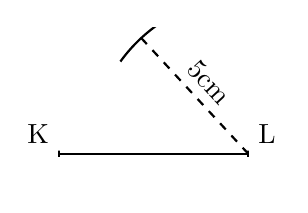
\begin{tikzpicture}[scale=0.4,every node/.style={scale=1}]
\clip (-1,-1) rectangle (7,4);%pour enlever les cercles «non tracés»
\draw[thick] (0,0) node [above left]{K}--+(90:0.1)--+(-90:0.1)--(0,0)--(6,0) node [above right]{L}--+(90:0.1)--+(-90:0.1);

\path [name path=cercle 1](0,0) circle (4.5cm);
\path [name path=cercle 2](6,0) circle (5cm);

\draw [name intersections={of=cercle 1 and cercle 2,by={I1,I2}}] 
   [dashed,thick] (I1) -- (6,0) node [midway,sloped,above]{5cm};
\begin{scope}
\clip (I1) circle (1);
\draw [thick](6,0) circle (5cm);
\end{scope}

\coordinate (L) at (6,0);
\begin{scope}[scale=0.65]
\Compas {L}{I1} 
\end{scope}

   
\end{tikzpicture} 
 & 
 
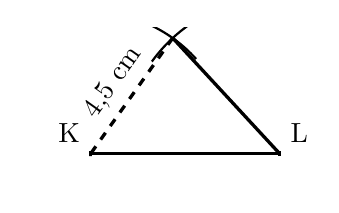
\begin{tikzpicture}[scale=0.4,every node/.style={scale=1}]
\clip (-2,-1) rectangle (7,4);%pour enlever les cercles «non tracés»

\draw[very thick] (0,0) node [above left]{K}--+(90:0.08)--+(-90:0.08)--(0,0)--(6,0) node [above right]{L}--+(90:0.08)--+(-90:0.08);

\path [name path=cercle 1](0,0) circle (4.5cm);
\path [name path=cercle 2](6,0) circle (5cm);

\draw [name intersections={of=cercle 1 and cercle 2,by={I1,I2}}];
\draw [very thick](I1) -- (6,0);
\draw [dashed,very thick] (I1) -- (0,0) node [midway,sloped,above]{4,5 cm};
   
\begin{scope}
\clip (I1) circle (1);
\draw [thick](6,0) circle (5cm);
\draw [thick](0,0) circle (4.5cm);
\end{scope}

\coordinate (K) at (0,0);
\begin{scope}[scale=0.65]
\Compas {K}{I1} 
\end{scope}

   
\end{tikzpicture} 
 \\ 
 On trace un segment $[KL]$ de longueur 6 cm. & Le point $M$ est à 5 cm du point $L$ : il appartient au cercle de centre $L$ et de rayon 5 cm. & Le point $M$ est à 4,5 cm du point $K$ : il appartient au cercle de centre $K$ et de rayon 4,5 cm. \\
\end{tabularx} \\

\end{exemple*1}

\exercice 
Construis un triangle $VOL$ tel que :

$VO = 4$ cm ; $OL = 6,3$ cm et $LV = 3,8$ cm.

\vspace{2cm}
%\correction

\exercice 
Construis un triangle \textbf{équilatéral} $EAU$ de 45 mm de côté.

\vspace{2cm}
%\correction

\exercice 
Construis le triangle $UNO$ \textbf{isocèle} en $U$ avec :

$UN = 8$ cm et $NO = 3,6$ cm.
%\correction
 
\end{methode*1}
%%%%%%%%%%%%%%%%%%%%%%%%%%%%%%%%%%%%%%%%%%%%%%%%%%%%%%%%%%%%%%%%%%%%%%%%%%%%%%%%%
\begin{methode*1}[Avec 2 longueurs et 1 angle]

 \begin{exemple*1}
Construis un triangle $BAS$ tel que :

$AB = 10,4$ cm ; $BS = 8$ cm et $\widehat{ABS} = 99^\circ$ : \\[1em]
\begin{tabularx}{\textwidth}{X|X|X}
 \includegraphics[width=3.3cm]{triangleABS} &  \includegraphics[width=3.5cm]{rapporteurBS} & \includegraphics[width=3.6cm]{regleABS} \\ 
 On effectue une figure à main levée en respectant la nature des angles (aigu ou obtus). & On construit un segment $[SB]$ de 8 cm de longueur. On trace un angle mesurant $99^\circ$ de sommet $B$ et de côté $[BS)$. & On place le point $A$ sur le côté de l'angle à 10,4 cm du point $B$. \\
\end{tabularx} \\

\end{exemple*1}

\exercice
Construis un triangle $LET$ tel que :

$\widehat{ETL} = 55^\circ$ ; $ET = 5$ cm et $TL = 4,3$ cm.
\vspace{4cm}
%\correction

\exercice
Construis un triangle $SEL$ tel que :

$SL = 6,4$ cm ; $\widehat{SLE}= 124^\circ$ et $LE = 7,9$ cm.
\vspace{2cm}
%\correction
 
\end{methode*1}
%%%%%%%%%%%%%%%%%%%%%%%%%%%%%%%%%%%%%%%%%%%%%%%%%%%%%%%%%%%%%%%%%%%%%%%%%%%%%%%%%
\begin{methode*1}[Avec 1 longueur et 2 angles]

 \begin{exemple*1}
Construis le triangle $GAZ$ tel que :

$AZ = 11,2$ cm ; $\widehat{GAZ} = 100^\circ$ et $\widehat{AZG} = 31^\circ$. \\[1em]
\begin{tabularx}{\textwidth}{X|X|X}
 \includegraphics[width=3.3cm]{triangleGAZ} &  \includegraphics[width=3.0cm]{rapporteurAZ} & \includegraphics[width=3.0cm]{rapporteurGAZ} \\ 
 On effectue une figure à main levée en respectant la nature des angles (aigu ou obtus). & On trace un segment $[AZ]$ de longueur 11,2 cm. On construit un angle de sommet $A$, de côté $[AZ)$ et mesurant $100^\circ$. & On construit un angle de sommet $Z$, de côté $[ZA)$ et mesurant $31^\circ$. Les côtés des deux angles se coupent au point $G$. \\
\end{tabularx} \\

\end{exemple*1}

\exercice
Construis le triangle $SUD$ tel que :

$UD = 6$ cm ; $\widehat{SUD} = 65^\circ$ ; $\widehat{SDU} = 36^\circ$.
\vspace{4cm}
%\correction

\exercice
Construis le triangle $EST$ tel que :

$ET = 4,6$ cm ; $\widehat{SET} = 93^\circ$ et $\widehat{ETS} = 34^\circ$.
\vspace{2cm}
%\correction
 
\end{methode*1}

\newpage
%%%%%%%%%%%%%%%%%%%%%%%%%%%%%%%%%%%%%%%%%%%%%%%%%%%%%%%%%%%%%%%%%%%%%%%%%%%%%%%%%
\prof{
\begin{activite}[Manipulation: les droites remarquables dans le triangle]
\underline{Le but:} A l'aide de ficelles, construire d'abord un triangle quelconque puis placer les droites remarquables. Nommer le point d'intersection de ces droites.

\underline{Attention:} Prévoir un lieu suffisamment grand pour que les élèves puissent travailler au sol, par groupe.\\

Constituer 4 groupes de travail.\\
\underline{Matériel(par groupe):}
\begin{itemize}
\item 1 grande corde "fermée"
\item 3 petites cordes colorées
\end{itemize}
\underline{Matériel(pour la classe):}
\begin{itemize}
\item lots étiquettes droites remarquables et points d'intersection
\item un appareil photo
\item le matériel de géométrie pour tracer au tableau
\end{itemize}
\underline{déroulement (version 1: découverte):} Prévoir 2 périodes de cours.\\
Donner à chaque groupe une corde "triangle" et un lot de trois cordes  "droites".
\begin{itemize}
\item \underline{médiatrices:} Demander aux élèves de placer une corde de telle sorte qu'elle coupe un côté du triangle en son milieu, perpendiculairement. Faire les 3 médiatrices. Distribuer une étiquette "médiatrices" et "centre du cercle circonscrit" à chaque groupe. Faire une photo.
\item \underline{médianes:} Demander aux élèves de placer une corde qui passe par un sommet du triangle et qui coupe le côté opposé en son milieu. Faire les 3 médianes. Distribuer une étiquette "médianes" et "centre de gravité" à chaque groupe. Faire une photo.
\item \underline{hauteurs:} Demander aux élèves de placer une corde qui passe par un sommet et qui coupe le côté opposé perpendiculairement. Faire les 3 hauteur. Distribuer une étiquette "hauteurs" et "orthocentre" à chaque groupe. Faire une photo.
\item \underline{bissectrices:} Demander aux élèves de placer une corde qui coupe l'angle en deux parties égales. Faire les 3 hauteurs. Distribuer une étiquette "hauteurs" et "centre du cercle inscrit" à chaque groupe. Faire une photo.\\\\
Le travail du professeur est alors de construire un livret contenant une photo d'illustration de chacune des droites, la définition et un schéma récapitulatif, personnalisé pour chaque groupe.
\end{itemize}
Attention: des explications complémentaires intermédiaires sont indispensables. Notamment préciser la nature de ces droite (demi-droite), en faisant bien attention que les cordes matérialisant les bissectrices partent du sommet de l'angle alors que les autre droites dépassent.
\underline{déroulement (version 2: bilan fin de séance):} Prévoir une période de cours.\\
Donner à chaque groupe une corde "triangle" et un lot de trois cordes  "droites".\\
Distribuer à chaque groupe une étiquette "droites".\\
Trois élèves doivent maintenir au sol les trois sommets du triangle. Les autres élèves du groupe, doivent alors placer le plus précisément possible, les trois droites remarquables indiquées sur leur étiquette.\\
Attention: il faut bien expliquer aux élèves "sommets" qu'ils ne doivent pas bouger sinon le triangle change et tout le travail est à recommencer.\\
Un fois que les trois droites sont matérialisées, les élèves appellent le professeur qui vérifie leur travail et les questionne sur le point d'intersection. On place en suite l'étiquette "p. d'intersection". On prend une photo souvenir!\\\\
Le travail du professeur est alors de construire un livret contenant une photo d'illustration de chacune des droites, la définition et un schéma récapitulatif.


\end{activite}
}



\newpage

%%%%%%%%%%%%%%%%%%%%%%%%%%%%%%%%%%%%%%%%%%%%%%%%%%%%%%%%%%%%%%%%%%%%%%%%%%%%%%%%%
%Médiatrice

 \begin{aconnaitre}
Les médiatrices des trois côtés d'un triangle sont \MotDefinition{concourantes}{}.

Leur point d'intersection est le centre du \MotDefinition{cercle circonscrit}{} au triangle. Ce cercle passe par les trois sommets du triangle.
\end{aconnaitre}

 \vspace{2em}
 
 \begin{methode*1}[Construire le cercle circonscrit à un triangle]
 
\begin{remarque}
Il suffit de tracer les médiatrices de deux côtés pour déterminer le centre du cercle circonscrit.
 \end{remarque}
 
 \begin{exemple*1}
Trace le cercle circonscrit au triangle $PAF$ :
 \begin{tabularx}{\textwidth}{X|X|X}
 \includegraphics[width=3.2cm]{triangleFAP} &  \includegraphics[width=3.2cm]{triangleFAOP} & \includegraphics[width=3.2cm]{triangle_cercleFAOP} \\ 
 On construit la médiatrice du segment $[AP]$. & On construit la médiatrice du segment $[FA]$. Soit $O$ le point d'intersection des deux médiatrices. & Le cercle circonscrit est le cercle de centre $O$ et de rayon $OA$ (ou $OF$ ou $OP$). \\
\end{tabularx} \\

\end{exemple*1}

\exercice
Construis le triangle $FEU$ tel que :

$FE = 6$ cm ; $EU = 3,7$ cm et $UF = 3,5$ cm. Trace le cercle circonscrit au triangle $FEU$.
\vspace{4cm}
%\correction

\exercice
Construis le triangle $EAU$ et son cercle circonscrit sachant que : $EA = 6,1$ cm ; $AU = 3$ cm et $UE = 4,9$ cm.

\vspace{2cm}
%\correction

\end{methode*1}

\begin{definition}
Dans un triangle, une \MotDefinition{médiane}{} est une droite qui passe par un sommet du triangle et par le milieu du côté opposé à ce sommet.

Les trois médianes d'un triangle sont concourantes en un point, noté G, et appelé \MotDefinition{centre de gravité}{} du triangle.
\end{definition}

\vspace{2em}

\begin{methode*1}[Construire le centre de gravité d'un triangle]

\begin{remarque}
Puisque les trois médianes sont concourantes, il suffit d'en tracer deux pour déterminer le centre de gravité.
 \end{remarque}

 \begin{exemple*1}
 Trace la centre de gravité du triangle $ABC$ :
 \begin{tabularx}{\textwidth}{X|X|X}
 \includegraphics[width=3.2cm]{CentreGravite1} &  \includegraphics[width=3.2cm]{CentreGravite2} & \includegraphics[width=3.1cm]{CentreGravite3} \\ 
 On trace le milieu de deux des côtés (ici I et J). & On trace les médianes passant par ces deux milieux & Le centre de gravité G est le point d'intertection des médianes. \\
\end{tabularx} \\

\end{exemple*1}

 
\exercice
Construis le triangle $CLE$ tel que 
$CL = 4,5$ cm ; $CE = 5,2$ cm et $\widehat{CLE} = 78^\circ$ puis trace son centre de gravité.
%\correction


\end{methode*1}


%%%%%%%%%%%%%%%%%%%%%%%%%%%%%%%%%%%%%%%%%%%%%%%%%%
%Hauteurs

\newpage

\begin{definition}
Dans un triangle, une \MotDefinition{hauteur}{} est une droite qui passe par un sommet du triangle et qui est perpendiculaire au côté opposé à ce sommet.

Les trois hauteurs d'un triangle sont concourantes en un point, noté H, et appelé \MotDefinition{orthocentre}{} du triangle.
\end{definition}

\vspace{2em}

\begin{methode*1}[Construire les hauteurs d'un triangle]

 \begin{exemple*1}
 Trace la hauteur relative au côté $[BR]$ :
 \begin{tabularx}{\textwidth}{X|X|X}
 \includegraphics[width=3.2cm]{triangleARB_1} &  \includegraphics[width=3.2cm]{triangleARB_2} & \includegraphics[width=3.1cm]{triangleARB_3} \\ 
 On positionne l'équerre perpendiculairement au côté $[BR]$. & On fait glisser l'équerre jusqu'au point $A$. Il faut parfois prolonger le côté $[BR]$. & La hauteur relative au côté $[BR]$ est la droite perpendiculaire au côté $[BR]$ et passant par $A$. \\
\end{tabularx} \\

\end{exemple*1}

\begin{remarque}
On dit aussi «hauteur issue du sommet $A$» pour nommer la hauteur relative au côté $[BR]$.
 \end{remarque}
 
\exercice
Construis le triangle $CAR$ tel que 
$CA = 4,6$ cm ; $AR = 4,3$ cm et $\widehat{CAR} = 102^\circ$ puis trace la hauteur issue de $R$ et celle issue de $C$.
\vspace{2cm}
%\correction
     
\exercice
Construis un triangle $TAX$ tel que 

$TA = 6,3$ cm ; $\widehat{TAX} = 57^\circ$ et $\widehat{ATX} = 63^\circ$ puis trace ses hauteurs.
\vspace{2cm}
%\correction

\exercice
Construis un triangle $BUS$ tel que :

$BU = 6,4$ cm ; $US = 4,8$ cm et $BS = 8$ cm. Trace les trois hauteurs de ce triangle.
%\correction

\end{methode*1}



%%%%%%%%%%%%%%%%%%%%%%%%%%%%%%%%%%%%%%%%%%%%%%%%%%
%Bissectrices

 \newpage
 
 \begin{aconnaitre}
Les trois bissectrices des angles d'un triangle sont concourantes. 

Leur point d'intersection est le \MotDefinition{centre du cercle inscrit}{} dans le triangle. Ce cercle est tangent aux trois côtés du triangle.
 \end{aconnaitre}
 
 \vspace{2em}
 
 \begin{methode*1}[Centre du cercle inscrit dans un triangle]
 
 \begin{remarque}
Il suffit de tracer les bissectrices de deux angles pour déterminer le centre du cercle inscrit.
 \end{remarque}
 
 \begin{exemple*1}
 Construis un triangle $MER$ et son cercle inscrit de centre $O$ :
 \begin{tabularx}{\textwidth}{X|X|X}
 \includegraphics[width=3.2cm]{triangleMRE} &  \includegraphics[width=3.2cm]{triangleMREK} & \includegraphics[width=3.2cm]{triangle_cercleMREK} \\ 
 On trace les bissectrices de deux des trois angles du triangle $MER$. Elles se coupent en $O$, le centre du cercle inscrit. & On trace la perpendiculaire à $(ME)$ passant par le point $O$. Elle coupe $[ME]$ en $K$. On obtient ainsi un rayon $[OK]$ du cercle inscrit dans le triangle $MER$. & On trace le cercle de centre $O$ passant par $K$. \\
 \end{tabularx} \\

\end{exemple*1}
 
 \exercice
Construis un triangle $RAS$ tel que 

$RA = 7$ cm ; $AS = 8$ cm et $RS = 9$ cm puis son cercle inscrit.
%\correction
 
 \end{methode*1}



\exercicesbase
\begin{colonne*exercice}
\input{Triangles/Triangles_exos_entrain.tex}
\end{colonne*exercice}


\exercicesappr
\begin{colonne*exercice}
\input{Triangles/Triangles_exos_approf}
\end{colonne*exercice}

\connaissances
\input{Triangles/Triangles_qcm.tex}

\TravauxPratiques % pour nous "travailler en groupe"
\input{Triangles/Triangles_en_groupe.tex}

\recreation
\input{Triangles/Triangles_fin_chap.tex}




%\themaC
%\chapter{Nombres entiers, \\ multiples, diviseurs}\label{ChNbEntiersMultDiv}
\begin{acquis} % enlever peut-être le lien internet
\begin{itemize}
\item trouver des diviseurs d'un nombre (et tous les diviseurs si ce nombre n'est pas trop grand);
\item trouver des multiples d'un nombre; 
\item décomposer un nombre en produits de facteurs premiers;
\item calculer avec des puissances;
\item calculer le PGCD de deux nombres entiers;
\item résoudre des problèmes nécessitant l'utilisation du PGCD;
\item calculer le PPMC de deux nombres entiers.
\end{itemize}
\end{acquis}

\activites

\input{NbsEntiers_Multiples_Diviseurs/NbsEntMultDivis_acti.tex}

\cours
\input{NbsEntiers_Multiples_Diviseurs/NbsEntMultDivis_cours.tex}

\exercicesbase
\begin{colonne*exercice}
\input{NbsEntiers_Multiples_Diviseurs/NbsEntMultDivis_exos_entrain.tex}
\end{colonne*exercice}


\exercicesappr
\begin{colonne*exercice}
\input{NbsEntiers_Multiples_Diviseurs/NbsEntMultDivis_exos_approf}
\end{colonne*exercice}

\connaissances
\input{NbsEntiers_Multiples_Diviseurs/NbsEntMultDivis_qcm.tex}

\TravauxPratiques % pour nous "travailler en groupe"
\input{NbsEntiers_Multiples_Diviseurs/NbsEntMultDivis_en_groupe.tex}

\pagebreak

\recreation
\input{NbsEntiers_Multiples_Diviseurs/NbsEntMultDivis_fin_chap.tex}




%\themaG
%\chapter{Quadrilatères}\label{ChQuadrilateres}

\begin{acquis} % enlever le lien internet
\begin{itemize}
\item citer les définitions d'un parallélogramme, d'un losange, d'un rectangle et d'un carré;
\item utiliser les propriétés des différents quadrilatères, en particulier celles de leurs diagonales;
\item tracer des quadrilatères particuliers à partir de leurs propriétés.
\end{itemize}
\end{acquis}

\activites

\input{Quadrilateres/Quadrilateres_acti.tex}

\cours
\prof
{Les exercices rituels de ce chapitre porteront sur les notations.\\
\newline

Voici un lien permettant de trouver le jeu \href{http://jeux2maths.fr/tripoly/}{TRIPOLY} sur le site de jeux2maths.fr. Il s'agit de lire les codages sans se fier au visuel et d'en déduire la nature d'une figure. Attention: ce jeu contient des cerfs-volants à retirer potentiellement de la partie.}


%%%%%%%%%%%%%%%%%%%%%%%%%%%%%%%%%%%%%%%%%%%%%%%%%%%%%%%%%%%%%
 
 \prof{
\begin{activite}[Jeu: "Qui est-ce?"]
\underline{Matériel:} 
Un papier avec le nom d’un élève préalablement bien choisi en secret par le professeur.\\
\underline{Mise en place:}
Pousser toutes les tables sur le côté afin de pouvoir utiliser l’espace de la classe.
Faire mettre tous les élèves au fond de la classe.\\
\underline{Consigne:}
Connaissez-vous le jeu du qui est-ce ? Il s’agit de récupérer des informations sur un personnage pour en découvrir l’identité.
Ici, on va faire la même chose. J’ai écris le prénom de l’un d’entre-vous dans ce papier (pour que vous soyez sûrs que je ne triche pas !). Je vais donner des informations à son sujet. Si vous êtes concernés, vous avancez d’un pas.
Je dois être capable de donner suffisamment d’informations utiles pour qu’à la fin il ne reste plus que la personne dont le prénom est écrit.\\
\underline{Activité:} 
Il/elle:
\begin{itemize}
    \item est élève en 6ème
    \item est un élève en 6eF...
    \item est une fille / un garçon
    \item est blond(e)
    \item porte des lunettes
    \item ...
\end{itemize}
\underline{Lien avec le chapitre:}
\begin{itemize}
    \item est-ce que toutes les \textcolor{G1}{filles} sont des \textcolor{G1}{Marie}?
    \item Est-ce que \textcolor{G1}{Marie} est une \textcolor{G1}{fille}?
    \item Est-ce que tous les \textcolor{G1}{6eF2} portent des \textcolor{G1}{lunettes}?
    \item Est-ce que tous les gens qui portent des \textcolor{G1}{lunettes} (dans cette salle) sont des \textcolor{G1}{6eF2}?
\end{itemize}
On constate que ça marche dans un sens mais pas dans l'autre.\\
\newline
Il en est de même pour les quadrilatères. Ils ont tous des caractéristiques (de propriétés) qui nous permettent de les classer en commençant par ceux qui en ont le moins jusqu’à celui qui en a le plus. A chaque étape, on ajoute une propriété qui permet de se rapprocher un petit peu plus du quadrilatère le plus complet.\\
\newline
On va essayer de faire ça pour les quadrilatères: construire la hiérarchie des quadrilatères.\\
\begin{itemize}
    \item est-ce que toutes les \textcolor{G1}{parallélogrammes} sont des \textcolor{G1}{carrés}?
    \item Est-ce que tous les \textcolor{G1}{carrés} sont des \textcolor{G1}{parallélogrammes}?
    \item Est-ce que tous les \textcolor{G1}{parallélogrammes} ont \textcolor{G1}{4 angles droits}?
    \item Est-ce que tous les quadrilatères qui ont \textcolor{G1}{4 angles droits} sont des \textcolor{G1}{rectangles}?
\end{itemize}

\end{activite}
}
 
 %%%%%%%%%%%%%%%%%%%%%%%%%%%%%%%%%%%%%%%%%%%%%%%%%%%%%%%%%%%%%

\section{Définitions des principaux quadrilatères particuliers}
RemarqueBN : j'ai placé la figure suivante ici pour voir si on en a besoin, sinon, on l'enlèvera :
\begin{tikzpicture}[every node/.style={scale=0.7}]
% définition des styles
\def\couleur{yellow!50}
\tikzstyle{quadri}=[draw,fill=\couleur,text=blue]
\tikzstyle{estun}=[->,>=latex,very thick,dotted]

%%%%% les nœuds %%%%%
%%%Quadrilatère
\node (Q) at (0,2) {Quadrilatère};
\coordinate[shift={(0mm,1mm)}] (Q1) at (Q.north west);
\coordinate[shift={(2mm,-1mm)}] (Q2) at (Q.north east);
\coordinate[shift={(-3mm,1mm)}] (Q3) at (Q.south east);
\coordinate[shift={(2mm,-2mm)}] (Q4) at (Q.south west);
\draw[fill=\couleur] (Q1)--(Q2)--(Q3)--(Q4)--cycle;
\node[blue] (Q) at (0,2) {Quadrilatère};
%%%Parallélogramme
\node[rectangle] (P) at (0,1) {Parallélogramme};
\coordinate[shift={(-3mm,0mm)}] (P1) at (P.north west);
\coordinate[shift={(-3mm,0mm)}] (P2) at (P.north east);
\coordinate[shift={(3mm,0mm)}] (P3) at (P.south east);
\coordinate[shift={(3mm,0mm)}] (P4) at (P.south west);
\draw[fill=\couleur] (P1)--(P2)--(P3)--(P4)--cycle;
\node[color=blue] (P) at (0,1) {Parallélogramme};
%%%Rectangle
\node[rectangle,quadri] (R) at (-1,0) {Rectangle};
%%%Losange
\node[shape=diamond,shape aspect=2,quadri] (L) at (1.5,0) {Losange};
%%%Carré
\node[quadri,minimum size=1.2cm] (C) at (0,-1) {Carré};
%%%Trapèze
\node (T) at (2,2) {Trapèze};
\coordinate[shift={(0mm,0mm)}] (T1) at (T.north west);
\coordinate[shift={(0mm,0mm)}] (T2) at (T.north east);
\coordinate[shift={(4mm,0mm)}] (T3) at (T.south east);
\coordinate[shift={(-2mm,0mm)}] (T4) at (T.south west);
\draw[fill=\couleur] (T1)--(T2)--(T3)--(T4)--cycle;
\node[blue] (T) at (2,2) {Trapèze};

%%%%% les flèches %%%%%
\draw[estun] (P)--(Q);
\draw[estun] (R.north)--(P);
\draw[estun] (L.north west)--(P);
\draw[estun] (C)--(R.south);
\draw[estun] (C)--(L.south west);
\coordinate[shift={(-1mm,0mm)}] (TFl) at (T.west);
\draw[estun] (TFl)--(Q);

%%%%%% la légende %%%%%
\draw[estun] (1,-1.2)--(2.3,-1.2)node[midway,above]{est un};
\end{tikzpicture}
\begin{definition}
Le \MotDefinition{quadrilatère}{} :
Un quadrilatère est un polygone (figure qui a plusieurs côtés) qui possède 4 côtés. Il est dit quelconque quand il ne possède aucune autre propriété (il n'a rien de particulier).\\
Il a donc 4 sommets et 4 angles.\\


\begin{minipage}[t]{0.50\linewidth}
\begin{center} \textbf{Quadrilatère convexe}\\
\begin{tikzpicture}[every node/.style={scale=0.7}]
    \draw (0,0) node[left]{C}--(1.7,0.8) node[above]{D}--(2.6,-0.7)node[right]{A}--(2.2,-1)node[below]{B}--cycle;
\end{tikzpicture}
\end{center}
\end{minipage}
\begin{minipage}[t]{0.50\linewidth}
\begin{center}\textbf{Quadrilatère concave}\\
\begin{tikzpicture}[every node/.style={scale=0.7}]
    \draw (0,0) node[left]{U}--(1.7,0.8) node[right]{B}--(1.3,-0.2)node[right=1mm]{L}--(2.4,-1)node[below]{E}--cycle;
\end{tikzpicture}
\end{center}
\end{minipage}
\end{definition}

Deux côtés qui possèdent un sommet commun sont appelés 
\textcolor{B2}{sommets consécutifs}. De même, deux sommets liés par un côté sont dits \textcolor{B2}{consécutifs}.\\
Deux sommets ou deux côtés non consécutifs d'un quadrilatère sont des \textcolor{B2}{sommets opposés} ou \textcolor{B2}{côtés opposés}.\\
Les segments qui joignent deux sommets non consécutifs d'un quadrilatère sont appelés \textcolor{B2}{les diagonales} du quadrilatère.
\begin{center}
   \begin{tikzpicture}[every node/.style={scale=0.6}]

%pour le tracé
%\draw[gray!30] (-5,-5) grid (5,5);
%\fill[red] (0,0) circle (3pt);

% définition des styles
\def\couleur{yellow!50}
\tikzstyle{quadri}=[draw,fill=\couleur,text=blue]

%carré
\begin{scope}[xshift=1.6cm,yshift=-0.2cm,scale=0.8,rotate=-10] 
\draw (0,0)--(1,0)--(1,1)--(0,1)--cycle;
%\draw (0.1,0)|-(0,0.1);
\end{scope}

%carré avec 4 côtés égaux
%\begin{scope}[xshift=1.8cm,yshift=-1cm,scale=0.8,rotate=10] 
%\draw (0,0)--(1,0)--(1,1)--(0,1)--cycle;
%\node at (0.5,0) {$\times$};
%\node at (1,0.5) {$\times$};
%\node at (0,0.5) {$\times$};
%\node at (0.5,1) {$\times$};
%\end{scope}

%losange avec 4 côtés égaux
\begin{scope}[xshift=3.8cm,yshift=0.8cm,rotate=-20] 
\draw (0,0)--(0.6,1)--(1.2,0)--(0.6,-1)--cycle;
\node at (0.3,0.5) {$\circ$};
\node at (0.9,0.5) {$\circ$};
\node at (0.9,-0.5) {$\circ$};
\node at (0.3,-0.5) {$\circ$};
\end{scope}

%losange avec diagonales perpendiculaires
\begin{scope}[xshift=5.3cm,yshift=-0.4cm,rotate=-45] 
\draw (0,0)--(0.6,1)--(1.2,0)--(0.6,-1)--cycle;
\draw (0,0)--(1.2,0);
\draw (0.6,1)--(0.6,-1);
\draw (0.7,0)|-(0.6,0.1);
\end{scope}

%rectangle avec 1 angle droit
\begin{scope}[xshift=-1.1cm,yshift=0.7cm,rotate=-15] 
\draw (0,0)--(0,.8)--(1.5,.8)--(1.5,0)--cycle;
\draw (0.1,0)|-(0,0.1);
\end{scope}

%rectangle avec diagonales de même longueur
\begin{scope}[xshift=-2.3cm,yshift=-1.2cm,rotate=40] 
\draw (0,0)--(0,.8)--(1.6,.8)--(1.6,0)--cycle;
\draw (0,0)--(1.6,0.8);
\draw (0,.8)--(1.6,0);
\node at (0.4,0.2) {$\circ$};
\node at (1.2,0.2) {$\circ$};
\node at (0.4,0.6) {$\circ$};
\node at (1.2,0.6) {$\circ$};
\end{scope}

%parallélogramme avec diagonales se coupant au milieu
\begin{scope}[xshift=-0.6cm,yshift=2.4cm,rotate=-10] 
\draw (0,0)--(0.4,.8)--(2,.8)--(1.6,0)--cycle;
\draw (0,0)--(2,0.8);
\draw (0.4,.8)--(1.6,0);
\node at (0.5,0.2) {$\circ$};
\node at (1.5,0.6) {$\circ$};
\node[rotate=50] at (0.7,0.6) {$\times$};
\node[rotate=50] at (1.3,0.2) {$\times$};
\end{scope}

%parallélogramme avec côtés opposés égaux
\begin{scope}[xshift=2.2cm,yshift=2cm,rotate=10] 
\draw (0,0)--(0.4,0.8)--(2,0.8)--(1.6,0)--cycle;
\node at (0.2,0.4) {$\circ$};
\node at (1.8,0.4) {$\circ$};
\node[rotate=0] at (1.2,0.8) {$\times$};
\node[rotate=0] at (0.8,0) {$\times$};
\end{scope}


%parallélogramme avec angles opposés égaux
\begin{scope}[xshift=1.5cm,yshift=-3cm,rotate=0] 
\draw (0,0)--(0.4,0.8)--(2,0.8)--(1.6,0)--cycle;
\end{scope}

%quadrilatère quelconque
\begin{scope}[xshift=5.8cm,yshift=-3cm,rotate=0] 
\draw (0,0)--(1,0.7)--(1.2,-0.15)--(0.5,-0.3)--cycle;
\end{scope}

%trapèze 1
\begin{scope}[xshift=-4.8cm,yshift=1.5cm,scale=0.8,rotate=20] 
\draw (0,0)--(0.8,0.6)--(1.8,0.6)--(2,0)--cycle;
\end{scope}

%trapèze 2
\begin{scope}[xshift=-4.8cm,yshift=1cm,scale=0.9,rotate=-20] 
\draw (0,0)--(0.1,0.4)--(0.7,0.4)--(1,0)--cycle;
\end{scope}

%cerf-volant avec diagonales perpendiculaires et côtés consécutifs égaux
\begin{scope}[xshift=7.6cm,yshift=1.5cm,rotate=10] 
\draw (0,0)--(0.5,0.6)--(1,0)--(0.5,-1.2)--cycle;
\draw (0,0)--(1,0);
\draw (0.5,0.6)--(0.5,-1.2);
\draw (0.6,0)|-(0.5,0.1);
\node[rotate=40] at (0.25,0.3) {$\times$};
\node[rotate=40] at (0.75,0.3) {$\times$};
\node[rotate=0] at (0.75,-0.6) {$\circ$};
\node[rotate=0] at (0.25,-0.6) {$\circ$};
\end{scope}


%%%%%%%% Éllipes des ensembles
\begin{scope}[xshift=0cm,yshift=0cm,rotate=0] 

%\tikzset{ellipse1/.pic={\draw [xscale=0.8,ultra thick,color=green] (0,0) circle (2);}}
%\tikzset{ellipse2/.pic={\draw [xscale=0.8,ultra thick,color=red] (0,0) circle (2);}}
%\pic at (5,0) {ellipse1};
%\pic at (6,0) {ellipse2};

\begin{scope} %coloration de la zone des carrés
\clip [xscale=1.6,yscale=1] (0,0) circle (2);
\fill[xscale=1.6,yscale=1,color=A3,opacity=0.3] (2.5,0) circle (2); 
\end{scope}

\draw[xscale=1.6,yscale=1,ultra thick,color=H2] (0,0) circle (2);
\draw[xscale=1.6,yscale=1,ultra thick, color=B2] (2.5,0) circle (2);
\draw[xscale=1.6,yscale=1,ultra thick, color=J2] (1.3,0) circle (3.5);
\draw[xscale=1.95,yscale=1.2,ultra thick, color=F2] (1,0) circle (4);
\end{scope}


%elipse autour des trapèzes
\node[draw,ultra thick, color=C1,shape=ellipse,minimum width=4cm,minimum height=3cm,rotate=50] (A) at (-4.2,1.5) {};
\node[text width=2cm,text centered] (B) at (-6,3){trapèzes : deux côtés opposés parallèles};
\draw (B) to [out=-90,in=90] (A);
\end{tikzpicture}
\end{center}

\begin{definition}
Le \MotDefinition{trapèze}{} est un quadrilatère dont \textcolor{C2}{\textbf{deux côtés opposés sont parallèles}}. \\
 \begin{center}
  \begin{tikzpicture}[rotate=0,every node/.style={scale=0.8}]
  \draw (-1,0) node[left]{A} -- (1,0) node[right]{B} -- (2,-1)node[right]{C} -- (-1.2,-1) node[left]{D} -- cycle;
\end{tikzpicture}
\end{center}

Les côtés parallèles du trapèze sont appelés \textcolor{C2}{\textbf{bases du trapèze}}.
\end{definition}

\begin{definition}
Le \MotDefinition{parallélogramme}{} est un quadrilatère dont les côtés opposés sont \textcolor{C2}{\textbf{parallèles deux à deux}}. \\
  \begin{center}
  \begin{tikzpicture}[rotate=10,every node/.style={scale=0.8}]
  \draw (-1,0) node[left]{A} -- (1,0) node[right=3pt]{B} -- (2,-1)node[right]{C} -- (0,-1) node[left=3pt]{D} -- cycle;
\end{tikzpicture}
\end{center}
\end{definition}

 
\begin{minipage}[t]{0.49\linewidth}
  \begin{definition}
   Le \MotDefinition{rectangle}{} est un parallélogramme qui a \textcolor{C2}{\textbf{1 angle droit}}.
  
\begin{center}
\begin{tikzpicture}[rotate=0,every node/.style={scale=0.8}]
\draw (-1,0) node[left]{A} -- (1,0) node[right]{B} -- (1,-1)node[right]{C} -- (-1,-1) node[left]{D} -- cycle;
\draw[very thick,color=C2] (-1,-0.2)-|(-0.8,0);
\end{tikzpicture}
\end{center}
 \end{definition}
 \end{minipage}
 %
 \begin{minipage}[t]{0.59\linewidth}
   \begin{definition}
   Le \MotDefinition{losange}{} un parallélogramme qui a \textcolor{C2}{\textbf{2 côtés consécutifs de même longueur}}.
   
\begin{center}
\begin{tikzpicture}[rotate=0,every node/.style={scale=0.8}]
\draw (-0.7,0) node[left]{A} -- (0,1) node[above]{B} -- (0.7,0)node[right]{C} -- (0,-1) node[below]{D} -- cycle;
\node[color=C2,rotate=45] at (-.35,.5){$\times$};
\node[color=C2,rotate=-45] at (.35,.5){$\times$};
%\node[color=C2,rotate=45] at (.35,-.5){$\times$};
%\node[color=C2,rotate=-45] at (-.35,-.5){$\times$};
\end{tikzpicture}
\end{center}
   \end{definition}
  \end{minipage} 
  
\begin{definition}
Le \MotDefinition{carré}{} est un parallélogramme qui a les propriétés du rectangle et du losange. \\

\begin{center}
\begin{tikzpicture}[rotate=0,every node/.style={scale=0.8}]
\draw (0,0) node[left]{A} -- (1,0) node[right]{B} -- (1,-1)node[right]{C} -- (0,-1) node[left]{D} -- cycle;
\draw[very thick,color=C2] (0,-0.2)-|(0.2,0);
\node[color=C2] at (.5,0){$\times$};
\node[color=C2] at (1,-.5){$\times$};
%\node[color=C2] at (.5,-1){$\times$};
%\node[color=C2] at (0,-.5){$\times$};
\end{tikzpicture}
\end{center}
\end{definition}

\section{Propriétés des principaux quadrilatères particuliers}

\begin{tikzpicture}
% définition des styles
\def\couleur{H4!50}
\def\echellequadri{1.2}
\def\echelleppte{0.8}
\tikzstyle{quadri}=[draw,color=H1,fill=\couleur,text=H1,scale=\echellequadri]
\tikzstyle{txtpptecote}=[text=A1,scale=\echelleppte,fill=white,text width=2cm,text badly centered]
\tikzstyle{txtpptediag}=[text=B2,scale=\echelleppte,fill=white,text width=2cm,text badly centered]
\tikzstyle{lignepptecote}=[->,>=latex,very thick,dotted,color=A1]
\tikzstyle{lignepptediag}=[->,>=latex,very thick,dotted,color=B2]


%%%%% les nœuds %%%%%
%%%Parallélogramme
\node[scale=\echellequadri] (P) at (0,4) {Parallélogramme};
\coordinate[shift={(-2mm,0mm)}] (P1) at (P.north west);
\coordinate[shift={(-2mm,0mm)}] (P2) at (P.north east);
\coordinate[shift={(2mm,0mm)}] (P3) at (P.south east);
\coordinate[shift={(2mm,0mm)}] (P4) at (P.south west);
\draw[color=H1,fill=\couleur] (P1)--(P2)--(P3)--(P4)--cycle;
\node[color=H1,scale=\echellequadri] (P) at (0,4) {Parallélogramme};
%%%Rectangle
\node[rectangle,quadri] (R) at (-3.2,0) {Rectangle};
%%%Losange
\node[shape=diamond,shape aspect=2,quadri] (L) at (4.2,0) {Losange};
%%%Carré
\node[quadri,minimum size=1.2cm] (C) at (0,-4) {Carré};

%%%%% les flèches avec le texte %%%%%
\draw[lignepptecote] (P) .. controls +(175:4cm) and +(160:4cm)..(R) node[txtpptecote,pos=0.7]{avec 2 côtés consécutifs perpendiculaires};

\draw[lignepptediag] (P) .. controls +(180:4cm) and +(90:0.6cm)..(R)node[txtpptediag,pos=0.6]{avec diagonales de même longueur};

\draw[lignepptecote] (P) .. controls +(10:4cm) and +(50:4cm)..(L)node[txtpptecote,pos=0.8]{avec 2 côtés consécutifs égaux};

\draw[lignepptediag] (P) .. controls +(0:3cm) and +(100:3cm)..(L)node[txtpptediag,pos=0.6]{avec diagonales perpendiculaires};

\draw[lignepptecote] (R) .. controls +(-130:4cm) and +(-160:4cm)..(C)node[txtpptecote,pos=0.4]{avec 2 côtés consécutifs égaux};

\draw[lignepptediag] (R) .. controls +(-70:3cm) and +(160:2cm)..(C)node[txtpptediag,pos=0.4]{avec diagonales perpendiculaires};

\draw[lignepptecote] (L) .. controls +(-50:3cm) and +(-20:3cm)..(C)node[txtpptecote,pos=0.4]{avec 2 côtés consécutifs perpendiculaires};

\draw[lignepptediag] (L) .. controls +(-110:3cm) and +(20:2cm)..(C)node[txtpptediag,pos=0.5]{avec diagonales de même longueur};

\end{tikzpicture}

\section{Méthodes de construction}

\begin{methode*1}[Construire un parallélogramme avec la règle et l'équerre]

\vspace{0.8em}
\textcolor{H1}{\textbf{Remarque}} : On utilise ici le fait que les côtés opposés sont parallèles deux à deux.

\begin{exemple*1}
Soient trois points $A$, $B$ et $C$ non alignés. Place le point $D$ tel que $ABCD$ soit un parallélogramme.\\[0.5em]


\begin{tabularx}{\textwidth}{X|X|X}
   \qquad \input{./Quadrilateres/figures/Parallelo_RegleEquerre_1} & \input{./Quadrilateres/figures/Parallelo_RegleEquerre_2} & 
\begin{tikzpicture}[every node/.style={scale=0.7}]
\draw[dashed](-0.8,0)--(1.2,0);
\draw[dashed](-0.8,1.2)--(1,1.2);
\draw[dashed](-0.92,1.39)--(.16,-0.23);
\draw[dashed](0.08,1.39)--(1.15,-.22);
\draw[thick,H1,densely dashed,->,>=stealth](.43,0.85)--(-0.26,0.39); 

\draw[thick] (0,0) node{$\times$} -- (1,0) node{$\times$} -- (0.2,1.2)node{$\times$};
\node[below right] at (0,0){A};
\node[below right] at (1,0){B};
\node[above right] at (0.2,1.2){C};
\node[above right] at (-0.8,1.2){D};
\node at (-0.8,1.2){$\times$};

%%%%%%%%%%%%%%%%%%%%%%%%
%%%%%%%%%%%%%%%%%%%%%%%%
%Début règle !! Si la figure est tournée, il faut
%rajouter l'angle de rotation dans le node des graduation
%pour que les nombres soient écrits correctement
%%%%%%%%%%%%%%%%%%%%%%%%
%%%%%%%%%%%%%%%%%%%%%%%% 

    %Graduation max. de la règle
    \def \Taille {6}
    %Définition de l 'angle de rotation de la règle
    \def \Rotation {-90-56.31}
    %Définition du décalage de la règle
    \def \DecalX {0.7}
    \def \DecalY {1.6}
    %Couleur des élèments de la règle (sauf le remplissage)
    \def \RegleColor {blue!60}

\begin{scope}[shift={(\DecalX,\DecalY)},rotate=\Rotation,scale=.35]
    % contours de la règle
    \draw[color=\RegleColor, fill =blue!5, opacity=0.5,rounded corners=2pt] (-0.2,0.5) rectangle (\Taille+0.2,-0.5);	%Dont couleur de remplissage
    % graduation 1 mm
    \foreach \a in {0,0.1,...,\Taille}{\draw[color=\RegleColor] (\a,0.5)--(\a,0.42);}
    % graduation 5 mm
    \foreach \a in {0,0.5,...,\Taille}{\draw[color=\RegleColor] (\a,0.42)--(\a,0.35);}
    % graduation et repères 10 mm
    \foreach \a in {0,1,...,\Taille}{\draw[color=\RegleColor] (\a,0.35)--(\a,0.25);}
\end{scope}

%%%%%%%%%%%%%%%%%%%%%%%%
%%%%%%%%%%%%%%%%%%%%%%%%
%Fin de la règle
%%%%%%%%%%%%%%%%%%%%%%%%
%%%%%%%%%%%%%%%%%%%%%%%%

%%%%%%%%%%%%%%%%%%%%%%%%
%%%%%%%%%%%%%%%%%%%%%%%%
%Définition des paramètres de l'équerre
%et de son positionnement
%%%%%%%%%%%%%%%%%%%%%%%%
%%%%%%%%%%%%%%%%%%%%%%%%

\def \xorigine {0.25}; %abscisse de l'origine de l'équerre posée avec un xshift
\def \yorigine {1.08}; %ordonnée de l'origine de l'équerre posée avec un yshift
\def \rotation {-90-56.31}; %angle de rotation de l'équerre
\def \longueur {4}; %longueur de l'équerre
\def \largeur {2}; %largeur de l'équerre
\def \epaisseur {\longueur * 0.1}; %épaisseur de la partie «colorée» de l'équerre

%%%%%%%%%%%%%%%%%%%%%%%%
%%%%%%%%%%%%%%%%%%%%%%%%
%Tracé de l'équerre
%%%%%%%%%%%%%%%%%%%%%%%%
%%%%%%%%%%%%%%%%%%%%%%%%

\begin{scope}[xshift=\xorigine cm,yshift=\yorigine cm,rotate=\rotation,scale=0.25]

%contour extérieur de l'équerre
\coordinate (A) at (0,0) ; %«origine» de l'équerre
\coordinate (B) at (\largeur,0) ;
\coordinate (C) at (0,\longueur) ;
\draw [gray](A)--(B)--(C)--cycle;


%contour intérieur de l'équerre
\coordinate (D) at (\epaisseur,\epaisseur) ;
\coordinate (E) at ($\largeur*(1,0)-{\largeur * \epaisseur / \longueur}*(1,0)-\epaisseur*(1,0)+\epaisseur*(0,1)$);
\coordinate (F) at ($\epaisseur*(1,0)+\longueur*(0,1)-{2*\longueur * \epaisseur / \largeur}*(0,1)$);
\draw [gray](D)--(E)--(F)--cycle;

%partie colorée de l'équerre
\fill [color=blue!50!gray,opacity=.4,even odd rule] (A)--(B)--(C)--cycle (D)--(E)--(F)--cycle;%l'option even odd rule permet de faire le remplissage entre les 2 zones définies

\end{scope}
%%%%%%%%%%%%%%%%%%%%%%%%
%%%%%%%%%%%%%%%%%%%%%%%%
%Fin de l'équerre
%%%%%%%%%%%%%%%%%%%%%%%%
%%%%%%%%%%%%%%%%%%%%%%%%

%%%%%%%%%%%%%%%%%%%%%%%%
%%%%%%%%%%%%%%%%%%%%%%%%
%Définition des paramètres de l'équerre
%et de son positionnement
%%%%%%%%%%%%%%%%%%%%%%%%
%%%%%%%%%%%%%%%%%%%%%%%%

\def \xorigine {-0.43}; %abscisse de l'origine de l'équerre posée avec un xshift
\def \yorigine {0.63}; %ordonnée de l'origine de l'équerre posée avec un yshift
\def \rotation {-90-56.31}; %angle de rotation de l'équerre
\def \longueur {4}; %longueur de l'équerre
\def \largeur {2}; %largeur de l'équerre
\def \epaisseur {\longueur * 0.1}; %épaisseur de la partie «colorée» de l'équerre

%%%%%%%%%%%%%%%%%%%%%%%%
%%%%%%%%%%%%%%%%%%%%%%%%
%Tracé de l'équerre
%%%%%%%%%%%%%%%%%%%%%%%%
%%%%%%%%%%%%%%%%%%%%%%%%

\begin{scope}[xshift=\xorigine cm,yshift=\yorigine cm,rotate=\rotation,scale=0.25]

%contour extérieur de l'équerre
\coordinate (A) at (0,0) ; %«origine» de l'équerre
\coordinate (B) at (\largeur,0) ;
\coordinate (C) at (0,\longueur) ;
\draw [gray](A)--(B)--(C)--cycle;


%contour intérieur de l'équerre
\coordinate (D) at (\epaisseur,\epaisseur) ;
\coordinate (E) at ($\largeur*(1,0)-{\largeur * \epaisseur / \longueur}*(1,0)-\epaisseur*(1,0)+\epaisseur*(0,1)$);
\coordinate (F) at ($\epaisseur*(1,0)+\longueur*(0,1)-{2*\longueur * \epaisseur / \largeur}*(0,1)$);
\draw [gray](D)--(E)--(F)--cycle;

%partie colorée de l'équerre
\fill [color=blue!50!gray,opacity=.4,even odd rule] (A)--(B)--(C)--cycle (D)--(E)--(F)--cycle;%l'option even odd rule permet de faire le remplissage entre les 2 zones définies

\end{scope}
%%%%%%%%%%%%%%%%%%%%%%%%
%%%%%%%%%%%%%%%%%%%%%%%%
%Fin de l'équerre
%%%%%%%%%%%%%%%%%%%%%%%%
%%%%%%%%%%%%%%%%%%%%%%%%

%%%%%%%%%%%%%%%%%%%%%%%%
%%%%%%%%%%%%%%%%%%%%%%%%
%Début crayon
%%%%%%%%%%%%%%%%%%%%%%%%
%%%%%%%%%%%%%%%%%%%%%%%%

\begin{scope}[xshift=-0cm,yshift=0cm,rotate=-20,scale=.15] %le crayon, xshift et yshift pour les coordonnées de la pointe, rotate pour l'orientation du crayon
\def \couleur {black}
\coordinate (O) at (0,0);
\fill[\couleur!40] (-0.2,4.8) -- (0.2,4.8) -- (0.2,0.8) --(0.1,0.65) -- (0,0.8) -- (-0.1,0.66) -- (-0.2,0.8) -- cycle; %corps du crayon
\draw[color=white] (0,4.8) -- (0,0.8); %trait intérieur du crayon
\fill[\couleur!90] (-0.2,4.3) -- (0,4.27) -- (0.2,4.3) -- (0.2,4.8) arc(30:150:0.23cm); %partie haute du crayon
\fill[brown!40] (-0.2,0.8) -- (O)node[coordinate,pos=0.75](a){} -- (0.2,0.8)node[coordinate,pos=0.25](b){} -- (0.1,0.65) -- (0,0.8) -- (-0.1,0.66) -- cycle; %pointe du crayon (partie taillée)
\fill[\couleur!90] (a) -- (O) -- (b) -- cycle; %mine du crayon
\end{scope}

%%%%%%%%%%%%%%%%%%%%%%%%
%%%%%%%%%%%%%%%%%%%%%%%%
%Fin crayon
%%%%%%%%%%%%%%%%%%%%%%%%
%%%%%%%%%%%%%%%%%%%%%%%%

\end{tikzpicture} \\ 
 
 
 On trace les côtés $[AB]$ et $[BC]$ du quadrilatère $ABCD$. Le quadrilatère $ABCD$ est un parallélogramme, donc ses côtés opposés sont parallèles deux à deux : soit $(AB) \parallel (CD)$. & On trace la parallèle à $(AB)$ passant par $C$. & On trace la parallèle à $(BC)$ passant par $A$. Ces deux droites sont sécantes en $D$.
 
 Ainsi $ABCD$ a ses côtés opposés parallèles deux à deux, c'est donc bien un parallélogramme. \\
\end{tabularx} \\[1em]

\end{exemple*1}

\exercice
Réalise un croquis avant de construire le parallélogramme $PRLG$ tel que $PR = 5$ cm, $PG = 6$ cm et  $\widehat{RPG} = 74^\circ$ en utilisant la propriété sur le parallélisme des côtés opposés du parallélogramme.
%\correction

\end{methode*1}

\newpage





\begin{methode*1}[Construire un parallélogramme avec le compas]

 
\vspace{0.8em}
\textcolor{H1}{\textbf{Remarque}} : On utilise ici le fait que les côtés opposés d'un parallélogramme sont égaux deux à deux.

 \begin{exemple*1}
 
  \begin{tabularx}{\textwidth}{X|X|X}
   \qquad \begin{tikzpicture}[every node/.style={scale=0.7}]
\draw [thick](0,0) node{$\times$} -- (1,0) node{$\times$} -- (0.2,1.2)node{$\times$};
\node[below left] at (0,0){A};
\node[below right] at (1,0){B};
\node[above right] at (0.2,1.2){C};

\end{tikzpicture} &   \qquad \begin{tikzpicture}[every node/.style={scale=0.7}]

\draw [thick](0,0) node{$\times$} -- (1,0) node{$\times$} -- (0.2,1.2)node{$\times$};
\node[below left] at (0,0){A};
\node[below right] at (1,0){B};
\node[above right] at (0.2,1.2){C};

\draw (-0.8,1.2) arc (180:170:1);
\draw (-0.8,1.2) arc (180:190:1);

\coordinate (C) at (0.2,1.2);
\coordinate (D) at (-0.8,1.2);
\begin{scope}[scale=0.2]
\Compas {C}{D} 
\end{scope}
\end{tikzpicture} &   \begin{tikzpicture}[every node/.style={scale=0.7}]

\draw [thick](0,0) node{$\times$} -- (1,0) node{$\times$} -- (0.2,1.2)node{$\times$};
\node[below left] at (0,0){A};
\node[below right] at (1,0){B};
\node[above right] at (0.2,1.2){C};
\node[above right] at (-0.8,1.2){D};

\draw[dashed](0,0)--(-0.8,1.2);
\draw[dashed](0.2,1.2)--(-0.8,1.2);

\draw (-0.8,1.2) arc (180:170:1);
\draw (-0.8,1.2) arc (180:190:1);
\draw (-0.8,1.2) arc (123.69:113.69:1.44);
\draw (-0.8,1.2) arc (123.69:133.69:1.44);

\coordinate (A) at (0,0);
\coordinate (D) at (-0.8,1.2);
\begin{scope}[scale=0.2]
\Compas {A}{D} 
\end{scope}
\end{tikzpicture} \\ 
 On trace les côtés $[AB]$ et $[BC]$ du quadrilatère $ABCD$.
 
 Le quadrilatère $ABCD$ est un parallélogramme, donc ses côtés opposés $[AB]$ et $[CD]$ sont de la même longueur deux à deux : soit $AB = CD$ et $BC = AD$. & À l'aide du compas, on reporte la longueur $AB$ à partir du point $C$. & On reporte la longueur $BC$ à partir du point $A$. On place le point $D$ à l'intersection des deux arcs de cercle puis on trace les côtés $[AD]$ et $[CD]$.
 
Ainsi $ABCD$ a ses côtés opposés égaux deux à deux, c'est donc bien un parallélogramme.\\
\end{tabularx} \\
 
 \end{exemple*1}

\vspace*{1em}
Pour les deux exemples ci-dessous, faire un croquis avant de faire le tracé précis :\\[-2.5em]

\exercice
Construis le parallélogramme $DRAP$ tel que $DR = 6$ cm, $DP = 8$ cm et $\widehat{RDP} = 40^\circ$ en utilisant la propriété sur l'égalité des longueurs des côtés opposés du parallélogramme.
%\correction

\vspace{2.7cm}

\exercice
Construis un rectangle $ABCD$ tel que $AB = 3$ cm et $BC = 5$ cm.
%\correction

\end{methode*1}

%%%%%%%%%%%%%%%%%%%%%%%%%%%%%%%%%%%%%%%%%%%%%%%%%%%%%%%%%%%%

\begin{methode*1}[Construire un losange avec le compas]
 
\vspace{0.8em}
\textcolor{H1}{\textbf{Remarque}} : On utilise ici le fait qu'un losange a quatre côtés de même longueur.

\begin{exemple*1}
Construis un losange $ABCD$ de 6 cm de côté.\\[1em]
\begin{minipage}[c]{0.7\linewidth}
On fait d'abord un croquis. Dans un losange, les quatre côtés ont la même longueur. Ainsi, les triangles $ABD$ et $CBD$ sont \textbf{isocèles} respectivement en $A$ et $C$.
 \end{minipage} \hfill%
 \begin{minipage}[c]{0.24\linewidth}
  \includegraphics[width=2.6cm]{losange_croquis}
  \end{minipage} \\
  
\begin{tabularx}{\textwidth}{X|X}
\qquad \begin{tikzpicture}[scale=1.2,every node/.style={scale=0.8}]

\draw [thick](0,0) -- (1.5,0.5) node[midway,above,sloped]{6 cm};
\draw [thick] (1.5,0.5) -- (1.5,-.5);
\draw [thick](1.5,-0.5) -- (0,0) node[midway,below,sloped]{6 cm};
\node[left] at (0,0){A};
\node[above] at (1.5,0.5){B};
\node[below] at (1.5,-0.5){C};

\draw (0,0) arc (-161.57:-151.57:1.58);
\draw (0,0) arc (-161.57:-171.57:1.58);
\draw (0,0) arc (161.57:151.57:1.58);
\draw (0,0) arc (161.57:171.57:1.58);

\coordinate (A') at (0.11,-0.25);
\coordinate (B) at (1.5,0.5);
\begin{scope}[scale=0.3]
\Compas {B}{A'} 
\end{scope}
\end{tikzpicture} & \qquad \begin{tikzpicture}[scale=1.2,every node/.style={scale=0.8}]

\draw [thick](0,0) -- (1.5,0.5) -- (1.5,-.5) -- cycle;
\draw [thick](1.5,0.5)--(3,0) node[midway,above,sloped]{6 cm};
\draw [thick](3,0) -- (1.5,-0.5) node[midway,below,sloped]{6 cm};
\node[left] at (0,0){A};
\node[above] at (1.5,0.5){B};
\node[below] at (1.5,-0.5){C};
\node[right] at (3,0){D};

\draw (0,0) arc (-161.57:-151.57:1.58);
\draw (0,0) arc (-161.57:-171.57:1.58);
\draw (0,0) arc (161.57:151.57:1.58);
\draw (0,0) arc (161.57:171.57:1.58);

\draw (3,0) arc (-161.57+180:-151.57+180:1.58);
\draw (3,0) arc (-161.57+180:-171.57+180:1.58);
\draw (3,0) arc (161.57+180:151.57+180:1.58);
\draw (3,0) arc (161.57+180:171.57+180:1.58);

\coordinate (D') at (3.06,0.27);
\coordinate (B) at (1.5,0.5);
\begin{scope}[scale=0.3]
\Compas {B}{D'} 
\end{scope}
\end{tikzpicture} \\
 On trace un segment $[BD]$. On construit un triangle $ABD$ isocèle en $A$ tel que $AB = AD = 6$ cm. & On construit le triangle $CBD$ isocèle en $C$ tel que $CB = CD = 6$ cm. \\
\end{tabularx} \\

 \end{exemple*1}

\exercice
Construis un losange $VERT$ tel que $VE = 4,5$ cm et $ET = 6,9$ cm.
%\correction

\vspace{3.5cm}

\exercice
Construis un triangle $BOL$ isocèle en $B$ tel que $BO = 2,1$ cm et $OL = 3,4$ cm. Place le point $S$ pour que $BOSL$ soit un losange.
%\correction

\end{methode*1}

%%%%%%%%%%%%%%%%%%%%%%%%%%%%%%%%%%%%%%%%%%%%%%%%%%%%%%%%%%%%



\exercicesbase
\begin{colonne*exercice}
\input{Quadrilateres/Quadrilateres_exos_entrain.tex}
\end{colonne*exercice}


\exercicesappr
\begin{colonne*exercice}
\input{Quadrilateres/Quadrilateres_exos_approf}
\end{colonne*exercice}

\connaissances

\QCMautoevaluation{Pour chaque question, plusieurs réponses sont
  proposées.  Déterminer celles qui sont correctes.}

\begin{QCM}
  \begin{GroupeQCM}
    \begin{exercice}
      Si $T$ est le milieu d'un segment $[AD]$ et que $AD = 56$ mm alors \ldots
      \begin{ChoixQCM}{4}
      \item $T \in [AD]$
      
      et $TA = 28$ mm
      \item $TA = TD$
      \item \\[-1em]
      \includegraphics[width=2.6cm]{triangleATD}
      \item $[AD]$ est un diamètre du cercle de centre $T$ et de rayon 28 mm
      \end{ChoixQCM}
\begin{corrige}
     \reponseQCM{abd} 
   \end{corrige}
    \end{exercice}

  \begin{exercice}
      Si $ROSE$ est un losange alors \ldots
      \begin{ChoixQCM}{4}
      \item $[RE]$ est une diagonale
      \item $[OS]$ est une diagonale
      \item $[OS]$ est un côté
      \item $[RS]$ est une diagonale
      \end{ChoixQCM}
\begin{corrige}
     \reponseQCM{cd}
   \end{corrige}
    \end{exercice}

\begin{exercice}
      ABCD est une figure telle que (AB) est parlallèle à (CD), (AD) est parallèle à (BC), (AB) et (BC) sont perpendiculaires. ABCD est un:
      \begin{ChoixQCM}{4}
      \item carré
      \item losange
      \item rectangle
      \item parallélogramme
      \end{ChoixQCM}
\begin{corrige}
     \reponseQCM{c} 
   \end{corrige}
    \end{exercice}

\begin{exercice}
     Les côtés consécutifs d'un losange sont:
      \begin{ChoixQCM}{3}
      \item parallèles
      \item perpendiculaires
      \item de la même longueur
      \end{ChoixQCM}
\begin{corrige}
     \reponseQCM{c} 
   \end{corrige}
    \end{exercice}

\begin{exercice}
     Les diagonales d'un carré:
      \begin{ChoixQCM}{4}
      \item sont perpendiculaires
      \item sont parallèles
      \item ont la même longueur
      \item ont le même milieu
      \end{ChoixQCM}
\begin{corrige}
     \reponseQCM{acd} 
   \end{corrige}
    \end{exercice}

\begin{exercice}
      On sait que BLOC est un parallélogramme tel que (BO) et (LC) sont perpendiculaires. On peut dire que:
      \begin{ChoixQCM}{4}
      \item BLOC est un losange
      \item BLOC est un rectangle
      \item BLOC est un carré
      \item BLOC est un parallélogramme
      \end{ChoixQCM}
\begin{corrige}
     \reponseQCM{a} 
   \end{corrige}
    \end{exercice}

\begin{exercice}
      Un carré est un
      \begin{ChoixQCM}{4}
      \item losange
      \item rectangle
      \item parallélogramme
      \item quadrilatère
      \end{ChoixQCM}
\begin{corrige}
     \reponseQCM{abcd} 
   \end{corrige}
    \end{exercice}

\begin{exercice}
     On sait que ABCD est un parallélogramme tel que AC=BD. On peut en déduire que ABCD est un:
      \begin{ChoixQCM}{4}
      \item parallélogramme
      \item losange
      \item carré
      \item rectangle
      \end{ChoixQCM}
\begin{corrige}
     \reponseQCM{d} 
   \end{corrige}
    \end{exercice}

\begin{exercice}
À partir du codage du quadrilatère suivant, tracé à main levée : \hspace{0.5em} \raisebox{-0.5\height}{\begin{tikzpicture}[rotate=0,every node/.style={scale=1}]

\tikzstyle{MainLevee}=[decorate,decoration={random steps,amplitude=1pt,segment length=10pt}]

\coordinate (A) at (0,0);
\coordinate (B) at (45:1.8);
\coordinate (C) at (0:2);
\coordinate (D) at (-45:1.8);

\draw[MainLevee] (A) -- (B) -- (C) -- (D) --cycle;

\draw (45:0.3) arc (45:-45:0.3) node[midway]{$\circ$};
\draw (1.85,0.26) arc (119.74:240.27:0.3)node[midway]{$\circ$};

\draw (1.06,1.06) arc (-135:-61.74:0.3);
\draw (.99,.99) arc (-135:-61.74:0.4);
\draw (1.42,-1.0) arc (60.26:134:0.3);
\draw (1.47,-0.92) arc (60.26:134:0.4);

\end{tikzpicture}}, on peut affirmer que c'est un:
      \begin{ChoixQCM}{4}
      \item parallélogramme
      \item rectangle
      \item losange
      \item carré
      \end{ChoixQCM}
\begin{corrige}
     \reponseQCM{c} 
   \end{corrige}
    \end{exercice}
    
\end{GroupeQCM}
\end{QCM}

\begin{QCM}
  \begin{GroupeQCM}
\begin{exercice}
À partir du codage du quadrilatère suivant, tracé à main levée : \hspace{0.5em} \raisebox{-0.5\height}{\input{./Quadrilateres/figures/QCM_MainLevee_2}}, on peut affirmer que c'est un:
      \begin{ChoixQCM}{4}
      \item parallélogramme
      \item rectangle
      \item losange
      \item carré
      \end{ChoixQCM}
\begin{corrige}
     \reponseQCM{c} 
   \end{corrige}
    \end{exercice}

\begin{exercice}
À partir du codage du quadrilatère suivant, tracé à main levée : \hspace{0.5em} \raisebox{-0.5\height}{\input{./Quadrilateres/figures/QCM_MainLevee_3}}, on peut affirmer que c'est un:
      \begin{ChoixQCM}{4}
      \item parallélogramme
      \item rectangle
      \item losange
      \item carré
      \end{ChoixQCM}
\begin{corrige}
     \reponseQCM{c} 
   \end{corrige}
    \end{exercice}

\begin{exercice}
À partir du codage du quadrilatère suivant, tracé à main levée : \hspace{0.5em} \raisebox{-0.5\height}{\begin{tikzpicture}[rotate=0,every node/.style={scale=1}]

\tikzstyle{MainLevee}=[decorate,decoration={random steps,amplitude=1pt,segment length=10pt}]

\coordinate (A) at (0,0);
\coordinate (B) at (1.2,1.3);
\coordinate (C) at (2.3,0);
\coordinate (D) at (1.5,-1.5);
\coordinate (O) at (1.5,0); %le centre du losange

%%%%%Les marques d'égalité de longueurs sur les diagonales :
\coordinate (A') at (0.75,0); %le milieu de la diagonale [AO]
\coordinate (B') at (1.35,0.65);
\coordinate (C') at (1.9,0);
\coordinate (D') at (1.5,-0.75);
\node at (A'){$\circ$};
\node at (B'){$\alpha$};
\node at (C'){$\circ$};
\node at (D'){$\alpha$};
%%% Les marques d'égalité de longueurs sur 2 côtés
\draw (1.75,0.65) node[rotate=30] {$\times$};
\draw (1.9,-0.75) node[rotate=0] {$\times$};

\draw[MainLevee] (A) -- (B) -- (C) -- (D) --cycle;

\draw[MainLevee] (A)--(A'); 
\draw[MainLevee] (A')--(O);
\draw[MainLevee] (B)--(B'); 
\draw[MainLevee] (B')--(O);
\draw[MainLevee] (C)--(C'); 
\draw[MainLevee] (C')--(O);
\draw[MainLevee] (D)--(D'); 
\draw[MainLevee] (D')--(O);

\end{tikzpicture}}, on peut affirmer que c'est un:
      \begin{ChoixQCM}{4}
      \item parallélogramme
      \item rectangle
      \item losange
      \item carré
      \end{ChoixQCM}
\begin{corrige}
     \reponseQCM{c} 
   \end{corrige}
    \end{exercice}

\end{GroupeQCM}
\end{QCM}

  


\TravauxPratiques % pour nous "travailler en groupe"
\input{Quadrilateres/Quadrilateres_en_groupe.tex}

\pagebreak

\recreation
\input{Quadrilateres/Quadrilateres_fin_chap.tex}




%\themaC
%\chapter{Nombres relatifs}\label{ChNbRelatifs}
\begin{acquis}
\begin{itemize}
\item donner le signe d'un nombre relatif;
\item déterminer l'opposé d'un nombre relatif;
\item lire l'abscisse d'un point sur une droite graduée;
\item placer un point dont je connais l'abscisse sur une droite graduée;
\item donner la valeur absolue d'un nombre;
\item lire les coordonnées d'un point dans un repère;
\item placer un point dont je connais les coordonnées dans un repère;
\item comparer deux nombres relatifs de même signe ou de signes différents.
\end{itemize}
\end{acquis}

\activites

\input{NbsRelatifs/NbsRelatifs_acti.tex}

\cours
\prof
Dans ce cours, on prendra soin de faire le lien avec les ensembles de nombres. Faire un rappel grâce que schéma donné au début de cet ouvrage.

\section{Les nombres relatifs}

% remarque : pour qu'un mot se retrouve dans le lexique : \MotDefinition{asymptote horizontale}{} 

\vspace{4em}

\begin{center}
    \begin{tikzpicture}[every node/.style={scale=0.6}]



%contour immeuble
\draw[fill=gray!40!yellow] (0,-3) rectangle (4,6);
%cage ascenseur
\draw[fill=gray!20] (1.5,-3)rectangle (2.5,6);
%étages sous-sol
\foreach \y in {-2,-1,1}{\draw (0,\y)--(1.5,\y) (2.5,\y)--(4,\y);}
%rez de chaussée (couleur différente)
\draw[fill=yellow!30!white] (0,0) rectangle (1.5,1) (2.5,0) rectangle (4,1); 
%niveau du sol
\draw[fill=gray!80] (-1,0) rectangle (5,0.1);
%fenêtres étages
\foreach \y in {1,2,...,5}{\foreach \x in {0.3,0.9,2.8,3.4} {\draw[fill=blue!40] (\x,\y+0.2) rectangle (\x+0.3,\y+0.8);}}
%ascenseur
\draw[fill=white] (1.6,2) rectangle (2.4,3);
\draw (2.2,5.7) circle (2mm);
\draw[very thick](2,3)--(2,5.7);
\draw[very thick] (2,5.7) arc (180:-80:2mm);
%boutons ascenseur étages
\foreach \y in {1,2,...,5}{\node[draw,circle,minimum size=1cm,fill=H2,text=black,scale=1] at (5.5,\y+0.5){\y}; }
\node[draw,circle,minimum size=1cm,fill=A2,text=black,scale=1] at (5.5,0.5){0}; 
\node[minimum width=1.5cm,minimum height=1cm,rounded corners=4pt,draw,rectangle,fill=A2,text=black,scale=1] at (7,0.5){Rez de chaussée}; 
\foreach \y in {-1,-2,-3}{\node[minimum width=1cm,minimum height=1cm,rounded corners=4pt,draw,rectangle,fill=B2,text=black,scale=1] at (5.5,\y+0.5){\y}; }

%insertion personnages
\draw (1.8,2.3) node[santa,minimum size=0.6cm]{} ;
\draw (2.2,2.3) node[mexican,minimum size=0.6cm]{} ;
%\draw (4,0) node[duck,minimum size=1.5cm]{};


\end{tikzpicture}
\end{center}

\begin{definition}
Lorsqu'on effectue un déplacement, deux données sont importantes:
\begin{itemize}
    \item le sens du déplacement
    \item la longueur du déplacement
\end{itemize}

En mathématiques, ce déplacement est caractérisé par \textcolor{C2}{\textbf{un nombre relatif}}.\\
\end{definition}

%%%%%%%%%%%%%%%%%%%%%%%%%%%%%%%%%%%%%%%%%%%%%%%%%%%%%%%%%%%%%%%%%
\begin{definition}
On commence toujours à compter à partir de 0.\\
Lorsque que le nombre est \textbf{inférieur à 0} (à gauche ou en dessous de 0), on parle de \textcolor{C2}{\textbf{nombre négatif}} et on utilise un signe $-$ placé devant le chiffre.\\
Lorsque que le nombre est \textbf{supérieur à 0} (à droite ou en dessus de 0), on parle de \textcolor{C2}{\textbf{nombre positif}} et on peut alors utiliser un signe $+$ placé devant le chiffre mais ce n'est pas toujours obligatoire.\\
0 est le seul nombre à la fois positif et négatif.\\
\end{definition}



%%%%%%%%%%%%%%%%%%%%%%%%%%%%%%%%%%%%%%%%%%%%%%%%%%%%%%%%%%%%%%%%%
\begin{definition}
La valeur du déplacement est donnée par le chiffre placé après le signe. C'est ce qu'on appelle \textcolor{C2}{\textbf{ la valeur absolue}}.
Il s'agit de la distance entre 0 est le nombre relatif. Il existe une notation pour parler de la valeur absolue:|nombre|\\
Deux nombres relatifs qui ne diffèrent \textbf{que} par leur signe sont \textcolor{C2}{\textbf{opposés}}.
\end{definition}

\begin{methode*1}[Trouver la valeur absolue d'un nombre relatif]


\begin{exemple*1}
Donne la valeur absolue du nombre $-2$ :

$|-2|$ = 2.
\end{exemple*1}


\exercice
Donne la valeur absolue des nombres suivants : $+5$ ; $-7$ ; $+64,78$ et $-123,4$.
%\correction

\end{methode*1}


\begin{methode*1}[Savoir utiliser le vocabulaire]



\begin{exemple*1}
Quel est le signe du nombre $-3$ ? Quel est son opposé ? \\[1em]
Le signe de $- 3$ est $-$, il est négatif. Son opposé est $+ 3$ que l'on écrit aussi 3.
\end{exemple*1}

\exercice 
Donne le signe des nombres relatifs suivants :

$+1235$ ; $-587$ ; $0$ ; $-1$ ;  $3,5$ ; $-0,001$.
%\correction

\exercice 
Donne l'opposé des nombres relatifs suivants :

$-2,531$ ; $0$ ; $1,245$ ;  $-0,03$ et $0,003$.
%\correction

\end{methode*1}



%%%%%%%%%%%%%%%%%%%%%%%%%%%%%%%%%%%%%%%%%%%%%%%%%%%%%%%%%%%%%%%%%

\newpage


\begin{aconnaitre}
Tout point d'une droite graduée est repéré par un nombre relatif appelé son \textcolor{C2}{\textbf{abscisse}}.

\begin{tikzpicture}
\draw[->] (-6,0) -- (6,0);
\draw (0,.2) node[above] {$O$} ;
\draw (0,-.2) node[below] {$0$} ;
\draw (1,-.2) node[below] {$+1$} ;
\draw (-4,1) node {$A$} ;
\draw[->] (-4,.8) -- (-4,.2) ;
\draw (0,0) node {$|$} ; \draw (1,0) node {$|$} ; \draw (2,0) node {$|$} ; \draw (3,0) node {$|$} ; \draw (4,0) node {$|$} ; \draw (5,0) node {$|$} ;
\draw (-1,0) node {$|$} ; \draw (-2,0) node {$|$} ; \draw (-3,0) node {$|$} ; \draw (-4,0) node {$|$} ; \draw (-5,0) node {$|$} ;
\end{tikzpicture}

\end{aconnaitre}

\vspace{2em}


\begin{methode*1}[Repérer un point sur une droite graduée]



\begin{exemple*1}
Sur la droite graduée ci-dessus, lis l'abscisse du point $A$ : \\[1em]
\begin{minipage}[c]{0.4\linewidth}
Le point $A$ est à gauche de l'origine :

son abscisse est donc négative.

La distance du point $A$ au point $O$ est $4$.
 \end{minipage} \hfill%
 \begin{minipage}[c]{0.1\linewidth}
 \begin{center}\includegraphics[width=0.23cm]{accolade_droite}\end{center}
  \end{minipage} \hfill%
  \begin{minipage}[c]{0.4\linewidth}
  donc l'abscisse du point $A$ est $-4$.
   \end{minipage} \\
\end{exemple*1}


\begin{exemple*1}
Trace une droite graduée et place les points $B(+6)$ et $C(-5)$ : \\[1em]
\begin{minipage}[c]{0.4\linewidth}
L'abscisse du point $B$ est $+6$ donc
 \end{minipage} \hfill%
 \begin{minipage}[c]{0.1\linewidth}
 \begin{center}\includegraphics[width=0.23cm]{accolade_gauche}\end{center}
  \end{minipage} \hfill%
  \begin{minipage}[c]{0.4\linewidth}
  Son abscisse est positive : le point $B$ est donc à droite de l'origine.
  
  Sa distance à l'origine est de 6 unités.
  \end{minipage} \\[0.5em]

\begin{minipage}[c]{0.4\linewidth}
L'abscisse du point $C$ est $-5$ donc
 \end{minipage} \hfill%
 \begin{minipage}[c]{0.1\linewidth}
 \begin{center}\includegraphics[width=0.23cm]{accolade_gauche}\end{center}
  \end{minipage} \hfill%
  \begin{minipage}[c]{0.4\linewidth}
  Son abscisse est négative : le point $C$ est donc à gauche de l'origine. 
  
  Sa distance à l'origine est de 5 unités.
   \end{minipage} \\

\begin{tikzpicture}
\draw[->] (-5.5,0) -- (6.5,0);
\draw (0,.2) node[above] {$O$} ;
\draw (0,-.2) node[below] {$0$} ;
\draw (1,-.2) node[below] {$+1$} ;
\draw (-5,1) node {$C$} ; \draw[->] (-5,.8) -- (-5,.2) ;
\draw (6,1) node {$B$} ; \draw[->] (6,.8) -- (6,.2) ;
\draw (0,0) node {$|$} ; \draw (1,0) node {$|$} ; \draw (2,0) node {$|$} ; \draw (3,0) node {$|$} ; \draw (4,0) node {$|$} ; \draw (5,0) node {$|$} ;\draw (6,0) node {$|$} ;
\draw (-1,0) node {$|$} ; \draw (-2,0) node {$|$} ; \draw (-3,0) node {$|$} ; \draw (-4,0) node {$|$} ; \draw (-5,0) node {$|$} ;
\end{tikzpicture}

\end{exemple*1}


\exercice
Trace une droite graduée d'origine $O$, une unité valant 2 cm. Places-y les points $A$, $B$, $C$, $D$ et  $E$, $F$ d'abscisses respectives $+3$ ; $-2$ ; $+5$ ; $-3$ et $-1,5$ ; $+2,5$. Que peux-tu dire des abscisses de $A$ et $D$ ?
%\correction

\end{methode*1}

%%%%%%%%%%%%%%%%%%%%%%%%%%%%%%%%%%%%%%%%%%%%%%%%%%%%%%%%%%%%%%%%

\section{Comparaison}

\vspace{4em}

\begin{aconnaitre}
\MotDefinition{Comparer deux nombres}{}, c'est trouver lequel est le plus grand (ou le plus petit) ou dire s'ils sont égaux.
\end{aconnaitre}

\vspace{4em}

\begin{methode*1}[Comparer deux nombres relatifs]


\begin{exemple*1}
Compare 9,37 et 92,751 puis 81,36 et 81,357 :

On compare d'abord les \textbf{\textcolor{H1}{parties entières}} des deux nombres :
\begin{itemize}
 \item $\textbf{\textcolor{H1}{9}} < \textbf{\textcolor{H1}{92}}$ donc $9,37 < 92,751$.
 \item $81,357$ et $81,36$ ont la même partie entière. On compare alors les \textbf{\textcolor{B2}{parties décimales}} : $81,357 = 81+0,357$ et $81,36=81+0,36$ mais $0,36=0,360$.
 \end{itemize}
Or \textbf{\textcolor{B2}{360 millièmes}} est plus grand que \textbf{\textcolor{B2}{357 millièmes}} donc $81,36 > 81,357$.
\end{exemple*1}


\begin{exemple*1}
Écris un encadrement de 1,564 au dixième : \\[0.5em]
$1,564 = 1 + 0,500 + 0,064$ et 0,064 est plus petit que 1 dixième. Ainsi, 1,564 est compris entre $1 + 0,5$ et $1 + 0,5 + 0,1$ , soit $1 + 0,6$. \\[0.5em]
Donc un encadrement au dixième de 1,564 est : $1,5 < 1,564 < 1,6$.
\end{exemple*1}

\exercice
Compare les nombres suivants :
\begin{colenumerate}{3}
 \item $+5$ et $+9$ ;
 \item $-3$ et $+8$ ;
 \item $-6$ et $-12$ ;
 \item $-5$ et $-9$ ;
 \item $5,1$ et $-5,3$ ;
 \item $-6,2$ et $-6,4$.
 \end{colenumerate}
%\correction

\end{methode*1}


\newpage

\begin{aconnaitre}
\textbf{Deux nombres relatifs positifs} sont rangés dans l'ordre de leur valeur absolue.

Un \textbf{nombre relatif négatif} est inférieur à un \textbf{nombre relatif positif}.

\textbf{Deux nombres relatifs négatifs} sont rangés dans l'ordre inverse de leur valeur absolue.
\end{aconnaitre}

\vspace{4em}


\begin{methode*1}[Comparer des nombres relatifs]

\begin{exemple*1}
Compare les nombres $-9$ et $-7$ : \\[0.5em]
\begin{tabular}{ccl} 
 $-9$ et $-7$ & $\longrightarrow$ & On veut comparer deux nombres relatifs négatifs. \\
 $9 > 7$ & $\longrightarrow$ & On détermine les valeurs absolues de $-9$ et de $-7$ puis  \\
& & on les compare. \\
 $-9 < -7$ & $\longrightarrow$ & On range les nombres $-9$ et $-7$ dans l'ordre inverse de leur  \\
 & & valeur absolue. \\
 \end{tabular}
\end{exemple*1}


\exercice
Range dans l'ordre croissant les nombres suivants : 
\begin{colenumerate}{2}
 \item $+12$ ; 0 ; $-7$ ; $-5$ ; $+5$ ;
 \item $-8$ ; $+10$ ; $-14$ ; $-21$ ; $+3$ ; $-1$ ;
 \item $-24$ ; $-2,4$ ; $2,4$ ; 0 ; $-4,2$ ; $-4$ ;
 \item $-2,4$ ; $+2,3$ ; $-2,42$ ; $+2,33$ ; $-3,23$.
 \end{colenumerate}
%\correction

\end{methode*1}
%%%%%%%%%%%%%%%%%%%%%%%%%%%%%%%%%%%%%%%%%%%%%%%%%%%%%%%%%%%%%%%%%
\newpage


\section{Repérage dans un plan}

\vspace{3em}

\begin{definition}
Dans un plan muni d'un repère, tout point est repéré par un couple de nombres relatifs appelé ses \MotDefinition{coordonnées}{} : la première est l'\textcolor{C2}{\textbf{abscisse}} (déplacement horizontal) et la seconde est l'\textcolor{C2}{\textbf{ordonnée}} (déplacement vertical).\\
Pour un point A, on écrira toujours \textbf{A(abscisse de A ; ordonnée de A)}.
\end{definition}

\vspace{3em}

\begin{methode*1}[Repérer un point dans un plan]

\begin{exemple*1}
Lis les coordonnées du point $A$ et du point $B$ puis place les points $C(5 ; -3)$ et $D(-3 ; 0)$ :

\begin{center} 
\begin{tikzpicture}[general,scale=0.5]
\draw[xstep=1,ystep=1,color=gray!80] (-6,-4) grid (6,4);
\axeX{-6}{6}{1}
\axeY{-4}{4}{1}

\draw[ultra thick,loosely dotted,color=C1](-4,2)--(0,2);
\node[right,color=C1,font=\bfseries] at (0,2){$+2$};
\draw[ultra thick,loosely dotted,color=G1](-4,2)--(-4,0);
\node[below,color=G1,font=\bfseries] at (-4,0){$-4$};

\node at (0,-3){$\bullet$};
\node[above left,font=\bfseries] at (-4,2){A};
\node at (-4,2){$\bullet$};
\node[right,font=\bfseries] at (0,-3){B};
\end{tikzpicture}
\end{center}

Pour lire les coordonnées du point $A$, on repère l'abscisse de $A$ sur l'axe horizontal (pointillés bleus) puis  son ordonnée sur l'axe vertical (pointillés violets). On conclut en donnant l'abscisse puis l'ordonnée : $A (-4 ; +2)$. \\[0.5em]
Le point $B$ appartient à l'axe des ordonnées donc son abscisse est 0. Ses coordonnées sont $(0 ; -3)$.

Pour placer le point $C$, on repère tous les points d'abscisse $+5$ puis on repère tous les points d'ordonnée $-3$. On place le point $C$ à l'intersection des deux lignes. \\[0.5em]
L'ordonnée du point $D$ est 0 donc $D$ appartient à l'axe des abscisses.
\end{exemple*1}

\exercice 

\begin{minipage}[c]{0.45\linewidth}
Sur la figure ci-contre, lis les coordonnées des points $K$, $L$, $M$, $N$, $P$ et $R$ :
 \end{minipage} \hfill%
 \begin{minipage}[c]{0.4\linewidth}
 \begin{center} 
\begin{tikzpicture}[general,scale=0.5]
\draw[xstep=1,ystep=1,color=gray!80] (-6,-4) grid (6,3);
\axeX{-6}{6}{1}
\axeY{-4}{3}{1}

\node at (-3,2){$\bullet$};
\node[left,font=\bfseries] at (-3,2){K};
\node at (-5,0){$\bullet$};
\node[below,font=\bfseries] at (-5,0){L};
\node at (2,-3){$\bullet$};
\node[left,font=\bfseries] at (2,-3){M};
\node at (0,1){$\bullet$};
\node[right,font=\bfseries] at (0,1){N};
\node at (4,-1){$\bullet$};
\node[left,font=\bfseries] at (4,-1){P};
\node at (-4,-3){$\bullet$};
\node[left,font=\bfseries] at (-4,-3){R};
\end{tikzpicture}
\end{center}
  \end{minipage} \\
%\correction

\exercice Trace sur ton cahier un repère d'origine $O$. L'unité de longueur est le centimètre sur les deux axes. Place les points suivants :
\begin{colenumerate}{4}
 \item $E(+2 ; +3)$ ;
 \item $F(-2 ; -3)$ ;
 \item $G(+2 ; -3)$ ;
 \item $H(-2 ; 3)$.
 \end{colenumerate}
%\correction

\end{methode*1}






\exercicesbase
\begin{colonne*exercice}
\input{NbsRelatifs/NbsRelatifs_exos_entrain.tex}
\end{colonne*exercice}


\exercicesappr
\begin{colonne*exercice}
\input{NbsRelatifs/NbsRelatifs_exos_approf}
\end{colonne*exercice}

\connaissances


\QCMautoevaluation{Pour chaque question, plusieurs réponses sont % enlever le lien internet
  proposées.  Déterminer celles qui sont correctes.}

\begin{QCM}
  \begin{GroupeQCM}
    \begin{exercice}
      Le nombre $-4$ est \ldots
      \begin{ChoixQCM}{4}
      \item positif
      \item négatif
      \item l'opposé de $4$
      \item la valeur absolue de $4$
      \end{ChoixQCM}
\begin{corrige}
     \reponseQCM{bc} 
   \end{corrige}
    \end{exercice}
    
    
    \begin{exercice}
      Le nombre 3 est \ldots
      \begin{ChoixQCM}{4}
      \item positif
      \item négatif
      \item ni positif ni négatif
      \item l'opposé de $-3$
      \end{ChoixQCM}
\begin{corrige}
     \reponseQCM{ad} 
   \end{corrige}
    \end{exercice}


    \begin{exercice}
      La valeur absolue de $-10$ est \ldots
      \begin{ChoixQCM}{4}
      \item positive
      \item négative
      \item $-10$
      \item $10$
      \end{ChoixQCM}
\begin{corrige}
     \reponseQCM{ad} 
   \end{corrige}
    \end{exercice}


    \begin{exercice}
      L'abscisse de $A$ est \ldots 
\vspace{-2em}
\begin{center}  \includegraphics[width=2.6cm]{axeAB} \end{center}

      \begin{ChoixQCM}{4}
      \item $-1$
      \item $-2$
      \item positive
      \item négative
      \end{ChoixQCM}
\begin{corrige}
     \reponseQCM{ad} 
   \end{corrige}
    \end{exercice}
    
    
     \begin{exercice}
      Sur la droite précédente, l'abscisse de $B$ est \ldots
      \begin{ChoixQCM}{4}
      \item l'opposé de celle de $A$
      \item la valeur absolue de $-2$
      \item la valeur absolue de celle de $A$
      \item positive
      \end{ChoixQCM}
\begin{corrige}
     \reponseQCM{bd} 
   \end{corrige}
    \end{exercice}
    

    \begin{exercice}
      L'abscisse de $B$ est \ldots \hspace{0.4em} l'abscisse de $A$. 
      
\vspace{-2em}
\begin{center} \includegraphics[width=2.6cm]{axeBA} \end{center}

      \begin{ChoixQCM}{4}
      \item plus grande que
      \item plus petite que
      \item $>$
      \item $<$
      \end{ChoixQCM}
\begin{corrige}
     \reponseQCM{bd} 
   \end{corrige}
    \end{exercice}
    
 
     \begin{exercice}
      $-3$ est \ldots 3
      \begin{ChoixQCM}{4}
      \item plus grand que
      \item plus petit que
      \item la valeur absolue de
      \item l'opposé de de
      \end{ChoixQCM}
\begin{corrige}
     \reponseQCM{bd} 
   \end{corrige}
    \end{exercice}
 \end{GroupeQCM}
\end{QCM}
 
 
\begin{QCM}
  \begin{GroupeQCM}   
    \begin{exercice}
      $-5$ \ldots $-7$
      \begin{ChoixQCM}{4}
      \item $>$
      \item $<$
      \end{ChoixQCM}
\begin{corrige}
     \reponseQCM{a}
   \end{corrige}
    \end{exercice}
    

    
    \begin{exercice}
      $-30$ \ldots $-35$
      \begin{ChoixQCM}{4}
      \item $>$
      \item $<$
      \end{ChoixQCM}
\begin{corrige}
     \reponseQCM{a}
   \end{corrige}
    \end{exercice}
    \begin{exercice}
      $-1,95$ \ldots $-1,94$
      \begin{ChoixQCM}{4}
      \item $>$
      \item $<$
      \end{ChoixQCM}
\begin{corrige}
     \reponseQCM{b}
   \end{corrige}
    \end{exercice}
    
    
    \begin{exercice}
      $-2,04$ \ldots $-2,048$
      \begin{ChoixQCM}{4}
      \item $>$
      \item $<$
      \end{ChoixQCM}
\begin{corrige}
     \reponseQCM{a}
   \end{corrige}
    \end{exercice} 

\end{GroupeQCM}
\end{QCM}

  


\TravauxPratiques % pour nous "travailler en groupe"
\input{NbsRelatifs/NbsRelatifs_en_groupe.tex}

\pagebreak

\recreation
\input{NbsRelatifs/NbsRelatifs_fin_chap.tex}




\themaG
\chapter{Périmètre, aire et volume}\label{ChPerimetresAires}

\begin{acquis}
\begin{itemize}
\item réaliser des conversions d'unités de longueurs;
\item réaliser des conversions d'unités d'aires;
\item calculer à partir d'une formule, l'aire d'un triangle, d'un carré, d'un rectangle, d'un parallélogramme, d'un trapèze ou d'un losange.
\end{itemize}
\end{acquis}

\activites

\input{PerimetresAires/PerimetresAires_acti.tex}

\cours
\section{Les 3 dimensions}
\begin{aconnaitre}
Une figure géométrique est représentée en une ou plusieurs dimensions:
\begin{center}
    \begin{tikzpicture} % longueur, surface et volune

%le segment (longueur)
\draw (0,0)--(2,0) node[scale=0.8,midway,above]{longueur} node[scale=0.8,midway,below]{1 dimension};
\draw (0,0)--+(0,0.15)--+(0,-0.15);
\draw (2,0)--+(0,0.15)--+(0,-0.15);

%le carré (surface)
\begin{scope}[xshift=3cm]
\draw[fill=A2] (0,0)--(2,0) node[scale=0.8,midway,below]{2 dimensions} --(2,2) --(0,2) node[scale=0.8,midway,above]{surface} -- cycle;
\end{scope}

%le cube (volume)
\begin{scope}[xshift=8cm]
\def \Width {2};
\def \Height {2};
\def \Depth {2};
\coordinate (O) at (0,0,0);
\coordinate (A) at (0,\Width,0);
\coordinate (B) at (0,\Width,\Height);
\coordinate (C) at (0,0,\Height);
\coordinate (D) at (\Depth,0,0);
\coordinate (E) at (\Depth,\Width,0);
\coordinate (F) at (\Depth,\Width,\Height);
\coordinate (G) at (\Depth,0,\Height);

\draw[blue,fill=blue] (O) -- (C) -- (G) -- (D) -- cycle;% Bottom Face
\draw[blue,fill=A2] (O) -- (A) -- (E) -- (D) -- cycle;% Back Face
\draw[blue,fill=pink] (O) -- (A) -- (B) -- (C) -- cycle;% Left Face
\draw[blue,fill=J1,opacity=0.8] (D) -- (E) -- (F) -- (G) -- cycle;% Right Face
\draw[blue,fill=J2,opacity=0.6] (C) -- (B) -- (F) -- (G) -- cycle;% Front Face
\draw[blue,fill=F,opacity=0.8] (A) -- (B) -- (F) -- (E) -- cycle;% Top Face


\path (C)--(G) node[scale=0.8,midway,below]{3 dimensions};
\path (A)--(E) node[scale=0.8,midway,above]{volume};

%\node at (A) {A};
%\node at (B) {B};
%\node at (C) {C};
%\node at (D) {D};
%\node at (E) {E};
%\node at (F) {F};
%\node at (G) {G};
\end{scope}

\end{tikzpicture}
\end{center}
\end{aconnaitre}


\section{Périmètre d'une figure}
\begin{aconnaitre}[Notion de longueur]
Le mot \MotDefinition{périmètre}{} désigne \textbf{\textcolor{H1}{la longueur}} du contour d'une figure.
\begin{center}
   \begin{tikzpicture} % pentagone avec côtés en couleur
\draw [very thick,color=blue] (0,0) node[color=black,below]{A} -- (1.5,0.5) (3,0)--(4.58,0);
\draw [very thick,color=red] (1.5,0.5) node[color=black,below right]{B} -- (1.5,1.5) (4.58,0)--(5.58,0);
\draw [very thick,color=pink] (1.5,1.5) node[color=black,right]{C} -- (0.5,2.5) (5.58,0)--(6.99,0);
\draw [very thick,color=green] (0.5,2.5) node [color=black,above]{D} -- (-0.5,1) (6.99,0)--(8.79,0);
\draw [very thick,color=yellow] (-0.5,1) node[color=black,left]{E} -- (0,0) (8.79,0)--(9.91,0);

\foreach \x / \y in {3/A,4.58/B,5.58/C,6.99/D,8.79/E,9.91/A}
    {\draw (\x,0) node[below=3pt]{\y} --+(0,0.15)--+(0,-0.15);}


\end{tikzpicture} 
\end{center}
Pour exprimer les longueurs, on utilise habituellement pour unité le \textbf{\textcolor{H1}{mètre}} et ses dérivés:
\begin{center}
    \begin{tabular}{|c|c|c|c|c|c|c|}
     \hline   km & hm & dam & m & dm & cm & mm \\ \hline
         & & & & & & \\
    \hline
    \end{tabular}
\end{center}
\end{aconnaitre}

\begin{methode*1}[Transformer des unités de longueurs]

\begin{exemple*1}
Transforme $0,5$ km en m.

Les m (mètres) sont l'unité de mesure.

$1$ km = $\numprint{1000}$ m, donc $0,5$ km $= 0,5 \cdot \numprint{1000}$ m = $500$ m
\end{exemple*1}

\exercice 
Effectue les conversions d'unités de longueur suivantes :
\begin{colenumerate}{3}
 \item $50$ cm en m ;
 \item $100$ mm en m ;
 \item $2,3$ hm en m ;
 \item $0,03$ dm en m ;
 \item $23$ dam en cm ;
 \item $4$ cm en hm.
 \end{colenumerate}
%\correction

\end{methode*1}
%%%%%%%%%%%%%%%%%%%%%%%%%%%%%%%%%%%%%%%%%%%%%%%%%%%%%%%

\section{Aire d'une figure géométrique} 

% remarque : pour qu'un mot se retrouve dans le lexique : \MotDefinition{asymptote horizontale}{} 

\begin{aconnaitre}[Notion de surface]
L' \MotDefinition{aire}{} désigne la valeur de \textbf{\textcolor{H1}{la surface}} occupée par une figure.\\
%le carré
\begin{center}
\begin{tikzpicture}
   \begin{scope}[xshift=3cm]
\draw[fill=blue] (0,0)--(2,0) --(2,2) --(0,2) -- cycle;
\end{scope}
\end{tikzpicture}
\end{center}

\prof{
Vous trouverez ici deux lien expliquant le développement du cube et permettant d'expliquer la surface du cube...\\
\href{https://www.geogebra.org/m/arvQstAW}{cube animé}\\
\href{https://www.geogebra.org/m/mZA5qKG9}{patron de cube}
}
Pour exprimer des aires, on utilise habituellement pour unité le \textbf{\textcolor{H1}{mètre carré}} et ses dérivés:
\begin{center}
    \begin{tabular}{|c|c|c|c|c|c|c|c|c|c|c|c|c|c|}
     \hline
     \multicolumn{2}{|c|}{$km^2$} & 
     \multicolumn{2}{c|}{$hm^2$} &
     \multicolumn{2}{c|}{$dam^2$} & 
     \multicolumn{2}{c|}{$m^2$} & 
     \multicolumn{2}{c|}{$dm^2$}  & 
     \multicolumn{2}{c|}{$cm^2$}  & 
     \multicolumn{2}{c|}{$mm^2$}  \\
     \multicolumn{2}{|c|}{} & 
     \multicolumn{2}{c|}{ha} &
     \multicolumn{2}{c|}{a} & 
     \multicolumn{2}{c|}{} & 
     \multicolumn{2}{c|}{}  & 
     \multicolumn{2}{c|}{}  & 
     \multicolumn{2}{c|}{}  \\ \hline
         & & & & & & & & & & & & & \\
    \hline
    \end{tabular}
\end{center}
\end{aconnaitre}

\begin{methode*1}[Pourquoi le tableau des aires comporte des doubles colonnes?]
\begin{exemple*1}\\
Prenons un longueur de 1$cm$.
\begin{tikzpicture} %segment de 1cm
\draw (0,0)--(1,0) node[scale=0.8,midway,above]{1 cm};
\draw (0,0)--+(0,0.15)--+(0,-0.15);
\draw (1,0)--+(0,0.15)--+(0,-0.15);
\end{tikzpicture}

Formons une surface basée sur sur cette longueur:
\begin{tikzpicture}%carré de 1cm^2
\draw (0,0)--(1,0) node[scale=0.8,midway,below]{$1 \text{cm}$} --(1,1) --(0,1) -- cycle;
\node[scale=0.8,rotate=90] at(-0.2,0.5) {$1 \text{cm}$};
\node[scale=0.8] at (0.5,0.5) {$1 \text{cm}^2$};
\end{tikzpicture}

L'aire de cette figure est de 1$cm^2$. \\

Maintenant, prenons une longueur dix fois plus grande c'est à dire 10$cm$ soit 1$dm$.\\
\begin{tikzpicture} %segment de 10cm
\draw (0,0)--(10,0) node[scale=0.8,midway,above]{10 cm} node[scale=0.8,midway,below]{1 dm};
\draw (0,0)--+(0,0.15)--+(0,-0.15);
\draw (10,0)--+(0,0.15)--+(0,-0.15);
\end{tikzpicture}

Formons une surface basée sur cette longueur:\\
\begin{tikzpicture}%carré de 100cm^2
\draw (0,0)--(10,0) node[scale=0.8,midway,below]{$10 \text{cm}$} --(10,10) --(0,10) -- cycle;
\node[scale=0.8,rotate=90] at(-0.2,5) {$10 \text{cm}$};
\node[scale=0.8] at (5,5) {$100 \text{cm}^2=1\text{dm}^2$};
\end{tikzpicture}

L'aire est alors de 100$cm^2$.\\
Que remarque-t-on?\\
Lorsqu'une longueur est multipliée par 10, l'aire qui lui est relative est multipliée par 100.\\
La double colonne dans le tableau des aires permet de retranscrire ce phénomène.
\end{exemple*1}
\exercice
Effectue les conversions d'unités d'aire suivantes:
\begin{colenumerate}{3}
 \item $7$ dm\up{2} en m\up{2} ;
 \item $200$ cm\up{2} en m\up{2} ;
 \item $3,2$ ha en m\up{2} ;
 \item $0,8$ dm\up{2} en m\up{2} ;
 \item $45$ hm\up{2} en dm\up{2} ;
 \item $400$ cm\up{2} en a.
 \end{colenumerate}
\end{methode*1}



\begin{methode*1}[Évaluer une aire]
\begin{exemple*1}
\begin{minipage}[c]{0.55\textwidth}
 À l'aide du quadrillage, détermine un encadrement de l'aire de la surface jaune, en prenant pour unité un carreau bleu.
 \end{minipage} \hfill%
 \begin{minipage}[c]{0.2\textwidth}
 \includegraphics[width=2.3cm]{aire1}
 \end{minipage} \\
 
 \begin{minipage}[c]{0.1\textwidth}
  \includegraphics[width=2.3cm]{aire2}
 \end{minipage} \hfill%
 \begin{minipage}[c]{0.7\textwidth}
La surface délimitée en \textbf{\textcolor{H1}{vert}} a une aire plus grande que celle délimitée par la courbe rouge. On compte le nombre de carreaux. Son aire est 18 carreaux.
 \end{minipage} \\[1em]
La surface délimitée en \textbf{noir} a une aire plus petite que celle délimitée par la courbe rouge. On compte le nombre de carreaux. Son aire est quatre carreaux.

Donc l'aire de la figure jaune est comprise entre 4 et 18 carreaux.

\end{exemple*1}

\exercice 
\begin{minipage}[c]{0.50\textwidth}
 Détermine l'aire, en nombre de carrés, des deux figures ci-contre.
 \end{minipage} \hfill%
 \begin{minipage}[c]{0.16\textwidth}
 \includegraphics[width=2.2cm]{aire3}
 \end{minipage} \\
%\correction
 
\end{methode*1}

%%%%%%%%%%%%%%%%%%%%%%%%%%%%%%%%%%%%%%%%%%%%%%%%%%%%%%%

\prof{
\begin{activite}[Problème à Dudu: peindre le cabanon]
\begin{partie}[objectif]
A ce stade, les élèves ne connaissent pas encore les formules de calcul d'aire. Le but est de leur faire découvrir par nécessité. Pour ce faire, ils peuvent avoir accès à différentes ressources bien que tout soit dans le livre.
\end{partie}
\begin{partie}[Mise en place]
Mettre les élèves par groupe de 4 environ.
\end{partie}

\begin{partie}[Consigne]
"on va regarder une vidéo. Tout est indiqué dans le film. Vous allez travailler ensemble pour essayer de répondre à la question qui va vous être posée". Chaque groupe devra rendre son travail qui explique clairement sa démarche sur une feuille A3 (et éventuellement la présenter à la classe!).\\
\end{partie}

\begin{partie}[La vidéo]
Voici le lien qui mène vers la vidéo:
\href{https://www.youtube.com/watch?v=ALUiqD4blG8}{Peindre le cabanon}.
On peut diffuser la vidéo à plusieurs reprises si nécessaire mais il est important que les élèves finissent par prendre des notes.
\end{partie}

\begin{partie}[Déroulement]
Après avoir regardé la vidéo 2 ou 3 fois, les élèves se mettent au travail.\\
Très vite, ils vont avoir besoin de formules qu'ils ne connaissent pas nécessairement. On peut alors les orienter vers les pages du livre correspondantes ou imaginer un prolongement à l'activité avec une tablette ou des ressources mises à disposition dans la classe.\\

Quand les élèves ont terminé, on peut imaginer une rapide présentation de leur travail à la classe. On peut afficher les travaux ou les noter...\\

Voici le genre de travail attendu....:
\begin{center}
\includegraphics[width=14cm]{PerimetresAires/figures/cabanon.eps} 
\end{center}

\end{partie}
\end{activite}
}

%%%%%%%%%%%%%%%%%%%%%%%%%%%%%%%%%%%%%%%%%%%%%%%%%%%%%%%

\section{Volume d'un solide}

\begin{aconnaitre}[Notion de volume]
Le mot \MotDefinition{volume}{} désigne l'espace contenu dans une figure en 3 dimensions.\\
Pour exprimer des volumes, on utilise habituellement pour unité le \textbf{\textcolor{H1}{mètre cube}} et ses dérivés:
\begin{center}
    \begin{tabular}{|c|c|c|c|c|c|c|c|c|c|c|c|c|c|c|c|c|c|c|c|c|}
     \hline
     \multicolumn{3}{|c|}{$km^3$} & 
     \multicolumn{3}{c|}{$hm^3$} &
     \multicolumn{3}{c|}{$dam^3$} & 
     \multicolumn{3}{c|}{$m^3$} & 
     \multicolumn{3}{c|}{$dm^3$}  & 
     \multicolumn{3}{c|}{$cm^3$}  & 
     \multicolumn{3}{c|}{$mm^3$}  \\    \hline
         & & & & & & & & & & & & & & & & & & & & \\
    \hline
    \end{tabular}
\end{center}
\end{aconnaitre}

\begin{methode*1}[Pourquoi le tableau des volumes comporte des triples colonnes?]
\begin{exemple*1}\\
On a vu précédemment que lorsque la longueur d'un carré est multipliée par 10, son aire est multipliée par 100.\\
Il en va de même avec les volumes. Lorsque la longueur d'un cube est multipliée par 10, le volume se trouve multiplié par 1000. C'est pour retranscrire ce phénomène que le tableau des volumes comporte des triples colonnes.
\end{exemple*1}
\exercice
Effectue les conversions d'unités de volume suivantes:
\begin{colenumerate}{3}
 \item $7,61$ km\up{3} en hm\up{3} ;
 \item $5,15$ m\up{3} en cm\up{3} ;
 \item $8,12$ cm\up{3}  en dm\up{3} ;
 \item $12,1$ m\up{3} en hm\up{3} ;
 \item $85,3$ hm\up{3} en dam\up{3} ;
 \item $48,7$ dam\up{3} en m\up{3}.
 \end{colenumerate}
\end{methode*1}


%%%%%%%%%%%%%%%%%%%%%%%%%%%%%%%%%%%%%%%%%%%%%%%%%%%%%%%%%%%%%%%%%
\begin{center}
    \textsc{\textbf{POUR RÉSUMER...}}\\
    \begin{tikzpicture} 
\def \Width {2};
\def \Height {2};
\def \Depth {2};

%les arrêtes du cube
\begin{scope}
\def \translate {0};
\coordinate (O) at (0+\translate,0,0);
\coordinate (A) at (0+\translate,\Width,0);
\coordinate (B) at (0+\translate,\Width,\Height);
\coordinate (C) at (0+\translate,0,\Height);
\coordinate (D) at (\Depth+\translate,0,0);
\coordinate (E) at (\Depth+\translate,\Width,0);
\coordinate (F) at (\Depth+\translate,\Width,\Height);
\coordinate (G) at (\Depth+\translate,0,\Height);

\draw[dashed, blue] (O) -- (A) (O) -- (C) (O) -- (D);% arrêtes cachées
\draw[blue] (D) -- (E) -- (F) -- (G) -- cycle;% Right Face
\draw[blue] (C) -- (B) -- (F) -- (G) -- cycle;% Front Face
\draw[blue] (A) -- (B) -- (F) -- (E) -- cycle;% Top Face

\path (C)--(G) node[scale=0.8,midway,below]{Les arrêtes du cube};

%\node at (A) {A};
%\node at (B) {B};
%\node at (C) {C};
%\node at (D) {D};
%\node at (E) {E};
%\node at (F) {F};
%\node at (G) {G};
\end{scope}

%les faces du cubes
\begin{scope}
\def \translate {4};

\coordinate (O) at (0+\translate,0,0);
\coordinate (A) at (0+\translate,\Width,0);
\coordinate (B) at (0+\translate,\Width,\Height);
\coordinate (C) at (0+\translate,0,\Height);
\coordinate (D) at (\Depth+\translate,0,0);
\coordinate (E) at (\Depth+\translate,\Width,0);
\coordinate (F) at (\Depth+\translate,\Width,\Height);
\coordinate (G) at (\Depth+\translate,0,\Height);

\fill[blue] (O) -- (C) -- (G) -- (D) -- cycle;% Bottom Face
\fill[green] (O) -- (A) -- (E) -- (D) -- cycle;% Back Face
\fill[pink] (O) -- (A) -- (B) -- (C) -- cycle;% Left Face
\fill[orange,opacity=0.8] (D) -- (E) -- (F) -- (G) -- cycle;% Right Face
\fill[yellow,opacity=0.6] (C) -- (B) -- (F) -- (G) -- cycle;% Front Face
\fill[red,opacity=0.8] (A) -- (B) -- (F) -- (E) -- cycle;% Top Face


\path (C)--(G) node[scale=0.8,midway,below]{les faces du cube};
%\path (A)--(E) node[scale=0.8,midway,above]{solide (ou volume?)};

%\node at (A) {A};
%\node at (B) {B};
%\node at (C) {C};
%\node at (D) {D};
%\node at (E) {E};
%\node at (F) {F};
%\node at (G) {G};
\end{scope}

%le cube
\begin{scope}
\def \translate {8};

\coordinate (O) at (0+\translate,0,0);
\coordinate (A) at (0+\translate,\Width,0);
\coordinate (B) at (0+\translate,\Width,\Height);
\coordinate (C) at (0+\translate,0,\Height);
\coordinate (D) at (\Depth+\translate,0,0);
\coordinate (E) at (\Depth+\translate,\Width,0);
\coordinate (F) at (\Depth+\translate,\Width,\Height);
\coordinate (G) at (\Depth+\translate,0,\Height);

%\draw (O) -- (C) -- (G) -- (D) -- cycle;% Bottom Face
%\draw (O) -- (A) -- (E) -- (D) -- cycle;% Back Face
%\draw (O) -- (A) -- (B) -- (C) -- cycle;% Left Face
\fill[green!50!black] (D) -- (E) -- (F) -- (G) -- cycle;% Right Face
\fill[green] (C) -- (B) -- (F) -- (G) -- cycle;% Front Face
\fill[green!50!white] (A) -- (B) -- (F) -- (E) -- cycle;% Top Face


\path (C)--(G) node[scale=0.8,midway,below]{Le cube};
%\path (A)--(E) node[scale=0.8,midway,above]{solide (ou volume?)};

%\node at (A) {A};
%\node at (B) {B};
%\node at (C) {C};
%\node at (D) {D};
%\node at (E) {E};
%\node at (F) {F};
%\node at (G) {G};
\end{scope}


\end{tikzpicture}

\end{center}

%%%%%%%%%%%%%%%%%%%%%%%%%%%%%%%%%%%%%%%%%%%%%%%%%%%%%%%%%%%%%%%%%

\newpage

\vspace{2em}
\section{Calculer des aires à l'aide d'une formule}

\begin{aconnaitre}[aire du rectangle et du triangle rectangle]
\begin{tabularx}{\linewidth}{|c|X|X|}
 \cline{2-3}
\multicolumn{1}{c|}{} & \begin{center} \textbf{\textcolor{H1}{Rectangle}} \includegraphics[width=2.5cm]{rectangleLI} \end{center} & \begin{center} \textbf{\textcolor{H1}{Triangle rectangle}} \includegraphics[width=2.7cm]{rectangleABCD4} \end{center} \\ \hline
Formule & L'aire du rectangle peut se calculer avec cette formule : {\large \textbf{$\mathcal{A} = L \cdot \ell$}} & L'aire de $ABD$ est égale à la moitié de l'aire de $ABCD$ : {\large \textbf{$\mathcal{A} = \dfrac{AB \cdot AD}{2}$}} \phantom{retourligne} \\\hline
 \end{tabularx} \\[1em]
Les longueurs doivent être exprimées dans la même unité.
\end{aconnaitre}
\begin{methode*1}
\begin{exemple*1}
Calcule l'aire de la figure $ABCDE$ ci‑dessous (L'unité de longueur est le centimètre) :
\begin{center}  \includegraphics[width=4.3cm]{aire4} \end{center}

 \begin{itemize}
  \item La figure est composée du rectangle $ABDE$ et du triangle rectangle $BCD$. Son aire est donc égale à la somme de l'aire de $ABDE$ et de l'aire de $BCD$ ;
  \item $\mathcal{A}_{ABDE} = AB \cdot AE = 7$ cm $\cdot$ $2,5$ cm = $17,5$ cm\up{2} ; \\[0.2em]
  \item $\mathcal{A}_{BCD} = \dfrac{BC \cdot BD}{2} = \dfrac{5,4 \text{ cm} \cdot 2,5 \text{ cm}}{2} = \dfrac{13,5 \text{ cm}\up{2}}{2} = 6,75 $ cm\up{2} ;\\[0.2em]
  \item $\mathcal{A}_{ABCDE} = 17,5$ cm\up{2} $+ 6,75$ cm\up{2} = $24,25$ cm\up{2}.
  \item L'aire de la figure $ABCDE$ est donc égale à $24,25$ cm\up{2}.
  \end{itemize}
\end{exemple*1}

\exercice 
Détermine l'aire d'un carré de côté 6 cm. 
%\correction

\exercice 
Détermine l'aire d'un rectangle de longueur 3 cm et de largeur 22 mm en donnant le résultat en cm\up{2}.
%\correction
     
\exercice 
$SON$ est un triangle rectangle en $S$, tel que 

$SO = 8,04$ dm et $SN = 0,93$ m. Détermine son aire en donnant le résultat en m\up{2}.
%\correction
 
\end{methode*1}
%%%%%%%%%%%%%%%%%%%%%%%%%%%%%%%%%%%%%%%%%%%%%%%%%%%%%%%%
\newpage

\vspace{2em}

\begin{aconnaitre}[Aire d'un triangle]
Pour calculer l’aire d’un triangle, on multiplie la \textbf{\textcolor{H1}{longueur d'un côté}} par la \textbf{\textcolor{C2}{hauteur}} relative à ce côté puis on divise le résultat par 2 :

\begin{tabularx}{\textwidth}{XX}
{\large $\mathcal{A} = \dfrac{b \cdot h}{2}$} & \includegraphics[width=5cm]{longueur_hauteur} \\
 \end{tabularx} \\
 \end{aconnaitre}

\vspace{4em}

\begin{methode*1}[Calculer l’aire d’un triangle]


 
\begin{exemple*1}
Calcule l’aire du triangle suivant :
\begin{minipage}[c]{0.68\textwidth}
\begin{itemize}
 \item On mesure la longueur d'un côté ;
 \item On mesure la hauteur relative à ce côté ;
 \item On multiplie la longueur du côté repéré par la hauteur relative à ce côté puis on divise le résultat par 2 : \\[0.3em]
$\mathcal{A} = \dfrac{10 \cdot 3}{2} = \dfrac{30}{2} = 15$. \\[0.3em]
L'aire du triangle vaut 15 cm\up{2}.
 \end{itemize}
 \end{minipage} \hfill%
 \begin{minipage}[c]{0.2\textwidth}
 \includegraphics[width=3.5cm]{triangle_croquisZ}
 \end{minipage} \\
\end{exemple*1}


\exercice 
Calcule l’aire des triangles suivants :
\begin{colenumerate}{2}
 \item
 
 \includegraphics[width=3.1cm]{triangle_croquisY}
 \item
 
 \includegraphics[width=2.8cm]{triangle_croquisW}
 \end{colenumerate}
%\correction

\end{methode*1}
%%%%%%%%%%%%%%%%%%%%%%%%%%%%%%%%%%%%%%%%%%%%%%%%%%%%%%%%
\newpage

\vspace{2em}

\begin{aconnaitre}[Aire d'un parallélogramme]
Pour calculer l’\MotDefinition{aire d’un parallélogramme}{}, on multiplie la \textbf{\textcolor{H1}{longueur d'un côté}} par la \textbf{\textcolor{C2}{hauteur}} relative à ce côté :

\vspace{1em}

\begin{tabularx}{\textwidth}{XX}
{\large $\mathcal{A} = b \cdot h$} & \includegraphics[width=4cm]{parallelogrammehb} \\
 \end{tabularx} \\

\end{aconnaitre}


\vspace{4em}

\begin{methode*1}[Calculer l’aire d’un parallélogramme]


\begin{exemple*1}
Détermine l’\textbf{aire} du parallélogramme suivant :
\begin{minipage}[c]{0.65\textwidth}
\begin{itemize}
 \item On mesure la \textbf{\textcolor{H1}{longueur}} d'un côté ;
 \item On mesure la \textbf{\textcolor{C2}{hauteur}} relative à ce côté ;
 \item On multiplie la longueur du côté repéré par la hauteur relative à ce côté : $\mathcal{A} = 12 \cdot 5 = 60$ ;
 \item L'aire du parallélogramme vaut 60 cm\up{2}.
 \end{itemize}
 \end{minipage} \hfill%
 \begin{minipage}[c]{0.26\textwidth}
 \includegraphics[width=3cm]{parallelog_croquis}
 \end{minipage} \\
\end{exemple*1}

\exercice 
Détermine l’aire des parallélogrammes $MNOP$ et $ABCD$ ci-dessous :
\begin{colenumerate}{2}
 \item 
 
 \includegraphics[width=3.7cm]{parallelogMNPO}
 \item 
 
 \includegraphics[width=4.4cm]{parallelogABCD}
 \end{colenumerate}
%\correction

\end{methode*1}
%%%%%%%%%%%%%%%%%%%%%%%%%%%%%%%%%%%%%%%%%%%%%%%%%%%%%%%%



\newpage

\vspace{2em}

\begin{aconnaitre}[Aire d'un losange]
Pour calculer l’aire d’un losange, on effectue le produit des \textbf{\textcolor{H1}{longueurs des diagonales}} puis on divise le résultat par 2 : 

\begin{tabularx}{\textwidth}{XX}
{\large $\mathcal{A} = \dfrac{d \cdot D}{2}$} & \includegraphics[width=5cm]{losangeDd} \\
 \end{tabularx} \\
 \end{aconnaitre}

\vspace{4em}

\begin{methode*1}[Calculer l’aire d’un losange]


 
 \begin{exemple*1}
Calcule l’aire du losange suivant :
\begin{minipage}[c]{0.68\textwidth}
\begin{itemize}
 \item On repère la longueur des diagonales.
 \item On calcule le produit des longueurs des diagonales puis on divise le résultat par 2 : \\[0.3em]
$\mathcal{A} = \dfrac{10 \cdot 5}{2} = \dfrac{50}{2} = 25$ \\[0.3em]
L'aire du losange vaut 25 cm\up{2}.
 \end{itemize}
 \end{minipage} \hfill%
 \begin{minipage}[c]{0.2\textwidth}
 \includegraphics[width=2.9cm]{losange26}
 \end{minipage} \\
\end{exemple*1}

 
 \exercice
Calcule l’aire des losanges suivants :
\begin{colenumerate}{2}
 \item
 
 \includegraphics[width=5cm]{losange12_10}
 \item
 
 \includegraphics[width=4cm]{losange10_10}
 \end{colenumerate}
%\correction

\end{methode*1}



\exercicesbase
\begin{colonne*exercice}
\input{PerimetresAires/PerimetresAires_exos_entrain.tex}
\end{colonne*exercice}


\exercicesappr
\begin{colonne*exercice}
\input{PerimetresAires/PerimetresAires_exos_approf}
\end{colonne*exercice}

\connaissances
\input{PerimetresAires/PerimetresAires_qcm.tex}

\TravauxPratiques % pour nous "travailler en groupe"
\input{PerimetresAires/PerimetresAires_en_groupe.tex}

\pagebreak

\recreation
\begin{enigme}[Invitation au bal]
Sur le carton d'invitation rectangulaire ci-contre, toutes les longueurs sont données en centimètres. Quel est le mot de passe ?
\vspace{1cm}
\begin{center} 
\begin{tikzpicture}[every node/.style={scale=1.2},scale=0.8]
 \draw (0,0)--(0,8)--(16,8)--(16,0)--cycle;
 \draw (8,8)--(8,0);
 \fill [yellow,opacity=0.3] (0,8)--(2.5,0)--(1.5,0)--cycle;
 \fill [yellow,opacity=0.3] (0,8)--(8,0)--(5.5,0)--cycle;
 
\draw (7.8,7.3) node[left,blue] {Cher AmienPoche,};
\draw (7.8,6.5) node[left,blue] {tu es notre invité};
\draw (7.8,5.9) node[left,blue] {pour une nuit};
\draw (7.8,5.4) node[left,blue] {costumée};
\draw (7.8,4.8) node[left,blue] {le 3 mars};

\draw (2,1.8) node[right,blue] {À};
\draw (2.2,1.1) node[right,blue] {partir};
\draw (2.4,0.5) node[right,blue] {de 18h};

\draw (12,6) node[purple] {Le code est};
\draw (12,5.4) node[purple] {l'aire en cm$^2$};
\draw (12,4.7) node[purple] {de la partie jaune};
\draw (12,4.2) node[purple] {du carton};
\draw (12,3.6) node[purple] {d'invitation};
\draw (12,2) node[purple] {L'équipe Sésamath};

\draw [thick,|<->|,>=stealth](-0.3,0)--(-0.3,8) node [midway,above,rotate=90]{16};
\draw [thick,|<->|,>=stealth](0,-0.3)--(1.5,-0.3) node [midway,below]{3};
\draw [thick,<->|,>=stealth](1.5,-0.3)--(2.5,-0.3) node [midway,below]{2};
\draw [thick,<->|,>=stealth](2.5,-0.3)--(5.5,-0.3) node [midway,below]{6};
\draw [thick,<->|,>=stealth](5.5,-0.3)--(8,-0.3) node [midway,below]{5};

\end{tikzpicture}

\end{center}
 
 \end{enigme}
 

 





\AfficheListeMethodes
\AfficheCorriges[2]
\AfficheLexique

\end{document}

%%% Local Variables: 
%%% mode: latex
%%% TeX-master: t
%%% End: 
